%%%%%%%%%%%%%%%%%%%%%%%%%%%%%%%%%%%%%%%%%%%%%%%%%%%%%%%%%%%%%%%%%%%%
%% texplate.tex
%% NOVA thesis document template
%%
%% This work is licensed under the 
%% Creative Commons Attribution-NonCommercial 4.0 International License. 
%% To view a copy of this license, 
%% visit http://creativecommons.org/licenses/by-nc/4.0/.
%%
%% Version 2017/07/26 [4.1.2]
%% Departamento de Informática
%% Faculdade de Ciências e Tecnologia
%% Universidade NOVA de Lisboa
%%
%% BUGS and SUGGESTIONS: please submit an issue at the project web page
%%      at: https://github.com/joaomlourenco/novathesis/
%%
%% HELP: please ask for help at the NOVAthesis google group at
%%          https://groups.google.com/forum/#!forum/novathesis
%%      or at the facebook page
%%          https://www.facebook.com/groups/novathesis/
%%
%% Authors / Contributors:
%%      - João Lourenço <joao.lourenco@fct.unl.pt>
%%      - Bruno Candeias <b.candeias@campus.fct.unl.pt>
%%
%% DONATIONS:
%%     If you think this templatze really helped you while writing your thesis,
%%     think about doing a small donation. Just access the website 
%%     https://github.com/joaomlourenco/novathesis/
%%     and click in the “Donation” link.
%%     I'll keep a list thanking to all the identified donors that identify
%%     themselves in the “*Add special instructions to the seller:*” box.
%%%%%%%%%%%%%%%%%%%%%%%%%%%%%%%%%%%%%%%%%%%%%%%%%%%%%%%%%%%%%%%%%%%%%

% The default option marked with (*)
\documentclass[
  docdegree=msc,        % phd(*), phdplan, phdprop, msc, mscplan, bsc
  school=nova/fct,      % nova/fct(*), nova/fcsh, nova/ims, ul/ist, ul/fc
  lang=en,              % en(*), fr, it, pt
  coverlang=en,         % defaults to main language
  copyrightlang=en,     % defaults to main language
  fontstyle=kpfonts,    % baskervaldx bookman charter ebgaramond fbb fourier garamond
                        % heuristica kpfonts(*) libertine mathpazo1 mathpazo2 newcent
                        % newpx newtx 
  chapstyle=elegant,    % bianchi bluebox brotherton dash default elegant(*) ell ger 
                        % hansen ist jenor lyhne madsen pedersen veelo vz14 vz34 vz43
  otherlistsat=front,   % front(*), back
  aftercover=false,     % false=don't true=include the aftercover file (even if exists)
  linkscolor=black,  % darkblue, black (Set to 'black' for PRINTING)
  printcommittee=true,  % set to 'false' from submitted versins who should not have 
                        % the list of committee memebers
  spine=false,          % (Set to 'true' for PRINTING the book spine)
  cdcover=false,         % (Set to 'true' for PRINTING the CD cover)
  biblatex={            % Options for biblatex (see biblatex documentation)
    %%%%%%%%%%%%%%%%%%%%%%%%%%%%%
    %%% uncomment for 'apa' like citations
    % backend=biber,    % must use biber as the backend (and not bibtex)
    % natbib=true,      % compatiblity with natbib (use \cite{…} or \citep{…})
    % style=apa,        % APA style
    % maxcitenames=2,   % use at most two names in citation
    %%%%%%%%%%%%%%%%%%%%%%%%%%%%%
    %%% uncomment for 'numeric-by-order-of-citation' like citations
    % backend=bibtex,     % use bibtex if possible
    % style=numeric-comp, % numeric(*), alphabetic, authoryear, bwl-FU
    % sortcites=true,     % If numeric, sort cites by crescent order
    % sorting=none,       % none, nyt(*), ynt
    %%%%%%%%%%%%%%%%%%%%%%%%%%%%%
    %%% uncomment for 'numeric-by-order-of-citation' like citations
    backend=bibtex,     % use bibtex if possible
    style=numeric-comp, % numeric(*), alphabetic, authoryear, bwl-FU
    sortcites=true,     % If numeric, sort cites by crescent order
    sorting=nyt,        % none, nyt(*), ynt
    %%%%%%%%%%%%%%%%%%%%%%%%%%%%%
    %%% uncomment for 'numeric-by-order-of-citation' like citations
    % backend=bibtex,   % use bibtex if possible
    % style=alphabetic, % numeric(*), alphabetic, authoryear, bwl-FU
    % sorting=nyt,      % none, nyt(*), ynt
    %%%%%%%%%%%%%%%%%%%%%%%%%%%%%
    %%% other options for biblatex
    maxbibnames=99,     % Never use 'et al' in the bibliography
    giveninits=true,    % render all first and middle names as initials
    hyperref=true       % Hyperlinks in citations: true(*) false
  },
  memoir={              % See the 'memoir' documentation
    %showtrims,          % DEBUG
    a4paper,            % the paper size/format
    11pt,               % 10pt, 11pt(*), 12pt
    final,              % draft, final  <= Replace 'draft' with 'final' in final version
  },
  media=screen,         % screen(*), paper
          % behavior to be defined in school options based in "\novathesis@opt@media"
          % definitions for screen: left and right margins are equal, colored links
          % definitions for paper: left and right margins are different, black links
]{novathesis}



%%============================================================
%%
%%  BEGINING OF USER COSTUMIZATION
%%
%%============================================================


%------------------------------------------------------------------
% Additional packages you may want to use (comment those not needed)
%------------------------------------------------------------------

%% VERY IMPORTANT
\usepackage{booktabs}    % Beautiful simple tables
\usepackage{paralist}    % To enable customizble enumerates
\usepackage{pdfpages}

\usepackage{tabularx,tabulary,multirow} %for tables

\usepackage{listings}     	% For pretty code
\usepackage{minted}			% For code highlighting
\usepackage{zi4}            	% Nice font


%% IMPORTANT (consider removing/commenting)
%\usepackage{colortbl}    % Use colors in background of table cells
\usepackage[textsize=footnotesize]{todonotes}  % To register TODO notes in the text
\setlength{\marginparwidth}{3.25cm}


%% FOR DEMO PURPOSES ONLY --- TO BE REMOVED by final users
%\usepackage{lipsum}


%------------------------------------------------------------------
% Costumization of some packages
%------------------------------------------------------------------

% Where to look for figures
% \prependtographicspath{{some-folder-here}}

% Setup of listings, for more information check the 'listings' package manual
% \lstset{
%     captionpos=t,
%     basicstyle={\ttfamily\footnotesize},
%     numbers=left,
%     numberstyle={\ttfamily\tiny},
%     tabsize=2,
%     language=Java,
%     float,
%     frame=single,
% }




%%============================================================
% For costumization,
%        see file 'nova-thesis/Schools/*/*/defaults.clo'
%        and file 'nova-thesis/lang-text.clo'
% You may override here any of the values defined there
% e.g.
% \majorfield[pt]={Engenharia Biomédica}
% \majorfield[en]={Biomedical Engineering}
% \thesiscover[msc,front]={cover-megi-nova-ims}
% \thesiscover[msc,front]={cover-mgi-nova-ims}
%%============================================================

% Title of the dissertation/thesis
% USe "\\" to break the title into two or more lines
% \let\oldtitle=\title
% \makeatletter
% \renewcommand{\title}[2][]{%
%   \ifthenelse{\equal{#1}{}}%
%     {\newcommand{\covertitle}{#2}}%
%     {\newcommand{\covertitle}{#1}}%
%   \let\title=\oldtitle
%   \title{#2}
% }
% \makeatother

\title[Replication and Caching Systems for the support of VMs stored in File Systems with Snapshots]{Replication and Caching Systems for the support of VMs stored in File Systems with Snapshots}
\subtitle{}

% Autor
% use [f] for female and [m] for male
\authorname[m]{Luís Miguel Teixeira da Silva}{Luís Miguel Silva}
\authordegree{Bachelor of Science}

% Date
\datemonth{November}
\dateyear{2018}


% Advisers
% use "\\&" if necessary to break the lines in the apprpriate place
% use [f] for female and [m] for male
\adviser[m]{Paulo Lopes}{Auxiliar Professor}{\\& NOVA University of Lisbon}  
% you may use "\newline" to force a new line
% \adviser[m]{John Doe Male Adviser Name}{Associate\\& Professor}{Some University Somewhere}
% \adviser[m]{John Doe Third Adviser Name}{Associate\\& Professor}{Some University Somewhere}


% Co-Advisers (maximum of 9)
% use [f] for female and [m] for male
\coadviser[m]{Pedro Medeiros}{Associate Professor}{\\& NOVA University of Lisbon}
% \coadviser[f]{[Nome da co-orientadora 2]}{[Profª.\ Auxiliar]}{[Universidade Nova de Lisboa]}


% committee (maximum of 9 elements)
% Use [c] for chair, [r] for raporteurs, [a] for advisers, [m] or nothing for remaining members
% Chair of the committee
\committee[c,f]{Prof. Carmen Pires Morgado}
% Main raporteurs
\committee[r,m]{Prof. Carlos Jorge de Sousa Gonçalves}
%\committee[r,f]{Name of another raporteur}
% Advisers
\committee[m,m]{Prof. Paulo Orlando Reis Afonso Lopes}
%\committee[a,f]{Name of another adviser}
% Other members of the committee - include the Adviser in this list
%\committee[m,m]{Another member of the committee}
%\committee[m,f]{Yet another member of the committee}

%%------------------------------------------------------------
%% All the names inside braces below sould correspond to a file
%%     with extension ".tex" and located in the "Chapters" folder
%%------------------------------------------------------------

% Dedicatory text. Will only be considered for final documents,
% i.e., "bsc", "msc" and "phd", otherwise, it will be silently ignored
%\dedicatoryfile{dedicatory}
% TODO Write dedicatory

% Acknowledgments text. Will only be considered for final documents,
% i.e., "bsc", "msc" and "phd", otherwise, it will be silently ignored
\acknowledgementsfile{acknowledgements}


% \quotefile{quote}    % Quote
\abstractfile[pt]{abstract-pt}  % Abstract in Portuguese
\abstractfile[en]{abstract-en}  % Abstract in English
%\abstractfile[fr]{abstract-fr}  % Abstract in French
\glossaryfile{glossary}
%\setglossarystyle{super}
\setglossarystyle{list}
\acronymsfile{acronyms}

% definition of the second cover, to be printed before the copyright (to serve FCSH-NOVA)
%\aftercoverfile{aftercover-nova-ims}


% The Table of Contents is always printed.
% The other lists below may be commented and omitted.
\addlisttofrontmatter{\listoffigures}  % The List of Figures. Comment to omit.
\addlisttofrontmatter{\listoftables}   % The List of Tables. Comment to omit.
%\addlisttofrontmatter{\lstlistoflistings}  % The List of Code Listings. Comment to omit.
\addlisttofrontmatter{\listoflistings}
\addlisttofrontmatter{\glsnogroupskiptrue\setlength{\glsdescwidth}{0.8\textwidth}\printnoidxglossaries}  % The Glossary and List of Acrnonyms


% Text chapters
% syntax: \chapterfile{file}
\chapterfile{chapter1}
\chapterfile{chapter2}
\chapterfile{chapter3}
\chapterfile{chapter4}
\chapterfile{chapter5}
\chapterfile{chapter6}
%\chapterfile{chapter7}


% Text appendixes
% sintax: \appendixfile{file}
% Comment if not needed
% \appendixfile{appendix1}
% \appendixfile{appendix2}

\annexfile{annex1}
\annexfile{annex2}
\annexfile{annex3}


% BibTeX bibiography files. Can be used multiple times with a single file nae each time.
\addbibfile{bibliography.bib}



%%==== DANGER ==== DANGER ==== DANGER ==== DANGER ==== DANGER ====
%%==== DANGER ==== DANGER ==== DANGER ==== DANGER ==== DANGER ====
%%==== DANGER ==== DANGER ==== DANGER ==== DANGER ==== DANGER ====
%%
%%  END OF USER COSTUMIZAITON
%% Please do not change below this point!!! :)
%%
%%==== DANGER ==== DANGER ==== DANGER ==== DANGER ==== DANGER ====
%%==== DANGER ==== DANGER ==== DANGER ==== DANGER ==== DANGER ====
%%==== DANGER ==== DANGER ==== DANGER ==== DANGER ==== DANGER ====

%% Begining of document
\begin{document}

%%%%%%%%%%%%%%%%%%%%%%%%%%%%%%%%%%%%%%%%%%%%%%%%%%%%%%%%%%%%%%
\thesisfrontmatter  % Before the main text (TOC, etc)
%%%%%%%%%%%%%%%%%%%%%%%%%%%%%%%%%%%%%%%%%%%%%%%%%%%%%%%%%%%%%%
\printcoverpage    % The cover page
\printaftercover
\printcopyright    % Print the copyright page (will only be printed if adequate for the document type)
\printdedicatory  % Print the dedicatory (will only be printed if adequate for the document type)
\printacknowledgements  % Print the acknowledgments (will only be printed if adequate for the document type)
\printquote        % Print the quote (if file exists and is adequate for the document type)
\printabstract    % Print abstracts (in PT and EN). The abstract in the document main language will
                  % be printed first, the abstract in the foreign language will be printed second
\printtoc         % Always print the table of contents
\printotherlists   % If option 'otherlistsat=front', print other lists of contents according
                  % to instructions given above, otherwise do nothing


%%%%%%%%%%%%%%%%%%%%%%%%%%%%%%%%%%%%%%%%%%%%%%%%%%%%%%%%%%%%%%
\thesismainmatter  % The main text
%%%%%%%%%%%%%%%%%%%%%%%%%%%%%%%%%%%%%%%%%%%%%%%%%%%%%%%%%%%%%%
\printchapthers    % Print document chapters
\printbib    % Print the bibliography
% \printotherlists   % Alternative location to print the other lists (if you uncomment this one, comment the other one above)
\printotherlists   % If option 'otherlistsat=back', print other lists of contents according to instructions given above, otherwise do nothing
\printappendixes  % Print appendixes, if any!
\printannexes  % Print appendixes, if any!
\printbackcoverpage

%%%%%%%%%%%%%%%%%%%%%%%%%%%%%%%%%%%%%%%%%%%%%%%%%%%%%%%%%%%%%%
%% End of document
%%%%%%%%%%%%%%%%%%%%%%%%%%%%%%%%%%%%%%%%%%%%%%%%%%%%%%%%%%%%%%
\end{document}

%%%%%%%%%%%%%%%%%%%%%%%%%%%%%%%%%%%%%%%%%%%%%%%%%%%%%%%%%%%%%%
%% Includes For Texpad
%%%%%%%%%%%%%%%%%%%%%%%%%%%%%%%%%%%%%%%%%%%%%%%%%%%%%%%%%%%%%%
%!TEX root = ../template.tex
%%%%%%%%%%%%%%%%%%%%%%%%%%%%%%%%%%%%%%%%%%%%%%%%%%%%%%%%%%%%%%%%%%%%
%% abstrac-pt.tex
%% NOVA thesis document file
%%
%% Abstract in Portuguese
%%%%%%%%%%%%%%%%%%%%%%%%%%%%%%%%%%%%%%%%%%%%%%%%%%%%%%%%%%%%%%%%%%%%

Nos últimos anos tem-se assistido a mudanças fundamentais na forma como a capacidade computacional é utilizada - com o grande aumento da utilização da virtualização, tanto a forma como são geridas as máquinas físicas como os modelos de infraestruturas num centro de dados sofreram grandes alterações. Estas mudanças são o resultado da procura por uma forma de disponibilizar rapidamente \textit{VMs} num ambiente altamente consolidado e com necessidades mínimas de intervenção humana na sua gestão.

Estão a ser desenvolvidas novas abordagens às técnicas de virtualização a um ritmo nunca visto, o que leva à existência de um ecossistema altamente volátil com novas plataformas e serviços a serem criados a todo o momento. É possível apreciar o esforço de grandes empresas da indústria das tecnologias de informação relativamente a problemas como a virtualização de desktops - com algum sucesso, mas ignorando completamente o poder de computação que está presente nos Personal Computers (PCs) instalados, optando por uma via de custo elevado, baseada em máquinas poderosas. Existe ainda espaço para melhores soluções e para o desenvolvimento de tecnologias que façam uso das capacidades de computação que já se encontrem presentes nas organizações, mantendo a simplicidade da sua configuração.

Esta tese foca-se no desenvolvimento de mecanismos de replicação e \textit{caching} para imagens de máquinas virtuais armazenadas num sistema de ficheiros local que tem a funcionalidade (pouco habitual) de suportar \textit{snapshots}. A arquitectura da solução proposta tem de ser distribuída e integrar-se na solução \textit{client-based VDI} já desenvolvida no projecto iCBD; tem de suportar eficientemente ficheiros com vários GB (alguns deles resultantes da criação de \textit{snapshots}) acedidos em leitura, e manter destes múltiplas versões. A solução desenvolvida tem ainda de oferecer desempenho, alta disponibilidade, e escalabilidade na presença de elevado número de clientes geograficamente distribuídos.



% Palavras-chave do resumo em Português
\begin{keywords}
	VDI, Sistema de Ficheiros Btrfs, Snapshots, Middleware de Replicação, Servidor de Caching.
\end{keywords}
% to add an extra black line

%!TEX root = ../template.tex
%%%%%%%%%%%%%%%%%%%%%%%%%%%%%%%%%%%%%%%%%%%%%%%%%%%%%%%%%%%%%%%%%%%%
%% abstrac-en.tex
%% NOVA thesis document file
%%
%% Abstract in English
%%%%%%%%%%%%%%%%%%%%%%%%%%%%%%%%%%%%%%%%%%%%%%%%%%%%%%%%%%%%%%%%%%%%

Over the span of a few years, there were fundamental changes in the way computing power is used. The heightening of virtualisation changed the infrastructure model of a \textit{data centre} and the way physical computers are managed. This shift is the result of enabling for fast deployment of Virtual Machines (VM) in a high consolidation ratio environment and with minimal need for management.

New approaches to virtualisation techniques are being developed at a surprisingly fast rate, which leads to an exciting and vibrating ecosystem of platforms and services seeing the light of day. We see big industry players engaging in such problems as \textit{Desktop Virtualisation} with moderate success, but completely ignoring the computation power already present in their clients, instead, opting for a costly solution of acquiring powerful new machines and software. There is still space for improvement and the development of technologies that take advantage of the onsite computation capabilities with minimum effort on the configuration side.

This thesis focuses on the development of mechanisms for the replication and caching of \textit{VM} images stored in a local file system, albeit one with the ability to perform snapshots. There are some particular items to address: like the solution needs to follow an entirely distributed architecture and fully integrate with a parallel implemented client-based Virtual Desktop Infrastructure (VDI) platform; needs to work with very large read-only files some of them resulting from the creation of snapshots while maintaining some versioning features. This work will also explore the challenges and advantages of deploying such a system in a high throughput network, maintaining high availability and scalability properties while supporting a broad set of clients efficiently. 


% Palavras-chave do resumo em Inglês
\begin{keywords}
	VDI, BTRFS, Snapshots, Replication Middleware, Cache Servers.
\end{keywords} 

%!TEX root = ../template.tex
%%%%%%%%%%%%%%%%%%%%%%%%%%%%%%%%%%%%%%%%%%%%%%%%%%%%%%%%%%%%%%%%%%%%
%% dedicatory.tex
%% NOVA thesis document file
%%
%% Simple dedicatory text (optional)
%%%%%%%%%%%%%%%%%%%%%%%%%%%%%%%%%%%%%%%%%%%%%%%%%%%%%%%%%%%%%%%%%%%%
\dedicatory

Lorem ipsum.

\enddedicatory
%!TEX root = ../template.tex
%%%%%%%%%%%%%%%%%%%%%%%%%%%%%%%%%%%%%%%%%%%%%%%%%%%%%%%%%%%%%%%%%%%%
%% acknowledgements.tex
%% NOVA thesis document file
%%
%% Text with acknowledgements
%%%%%%%%%%%%%%%%%%%%%%%%%%%%%%%%%%%%%%%%%%%%%%%%%%%%%%%%%%%%%%%%%%%%
\acknowledgements

The work presented in this document would never see the light of day if not for the collaboration of several people to whom I wish to manifest my profound gratitude and recognition.

Prof. Nuno Preguiça, Prof. Pedro Medeiros, Prof. Paulo Lopes


I also would like to acknowledge the following institutions for their hosting and financial support: \textit{Departamento de Informática and Faculdade de Ciências e Tecnologia of the Universidade NOVA de Lisboa} (DI-FCT NOVA); the \textit{NOVA Laboratory of Computer Science and Informatics} (NOVA LINCS) in particular the Computer Systems group; \textit{SolidNetworks – Business Consulting, LDA} of the \textit{Reditus S.A. Group}; and the funding provided through the \textit{COMPETE2020 / PORTUGAL2020} program for the \textit{iCBD} project (POCI-01-0247-FEDER-011467).
%!TEX root = ../template.tex
%%%%%%%%%%%%%%%%%%%%%%%%%%%%%%%%%%%%%%%%%%%%%%%%%%%%%%%%%%%%%%%%%%%
%% chapter1.tex
%% NOVA thesis document file
%%
%% Chapter with introduction
%%%%%%%%%%%%%%%%%%%%%%%%%%%%%%%%%%%%%%%%%%%%%%%%%%%%%%%%%%%%%%%%%%%
\newcommand{\novathesis}{\emph{novathesis}}
\newcommand{\novathesisclass}{\texttt{novathesis.cls}}


%%-------------------------------------------------------------------
%%	1 - Introduction
%%-------------------------------------------------------------------
\chapter{Introduction}
\label{cha:introduction}

%\begin{quotation}
%  \itshape
%  This work is licensed under the Creative Commons Attribution-NonCommercial~4.0 International License.
%  To view a copy of this license, visit \url{http://creativecommons.org/licenses/by-nc/4.0/}.
%\end{quotation}


%%-------------------------------------------------------------------
%%	1.1 - Context
%%-------------------------------------------------------------------
\section{Context} % (fold)
\label{sec:context}

The concept of virtualisation, despite all the recent discussion, isn’t new. In reality, this technology has been around since the 1960s~\cite{Buzen1973}, but it was not until the development of virtualisation technologies for the x86 architecture~\cite{Agesen2010} and the introduction of \textit{Intel VT}~\cite{Intel2010} and \textit{AMD SVM}~\cite{AMD2010} in the 2000s that virtualisation has entered the mainstream as the go-to technology solution for server deployment across many production environments. 

With efficient techniques that take advantage of all available resources, and a lowering price point on hardware, an opportunity for the advance of new application models and a revamp in the supporting infrastructure was generated. 

However, companies realised that the cost to run a fully fledged \textit{data centre} in-house is unreasonable and a cumbersome task. Not only taking into account the cost of the hardware, but factoring in the many requirements like the cooling systems that take care of the heat generated by the running machines, physical security to protect the rooms, fire suppressing systems in case of emergency, people to maintain the infrastructure, all added, result in considerable costs on a monthly basis.
Adding to this, the demand for instantaneous access to information and the extensive resources needed to store it does not stop growing.

This fact created an opening for a \gls{IaaS}~\cite{Mell2011} model, outsourcing all the responsibilities of storing the data and providing the needed computation resources from third parties, which are experts in maintaining huge data centres and even provide all this in various geographic regions.

With influential industry players following this trend, supporting more and more types of services and with an increasing number of customers joining this model, new ways to store the growing number of files have emerged. New file systems with a focus on reliability, consistency, performance, scalability, all in a distributed architecture are essential to a broad range of applications presenting a myriad of workloads.



%%-------------------------------------------------------------------
%%	1.2 - Motivation
%%-------------------------------------------------------------------
\section{Motivation} % (fold)
\label{sec:motivation}

Virtualisation is the pillar technology that allowed for the widespread of the IaaS cloud providers in a model of economies of scale. These cloud providers, such as Amazon AWS~\cite{aws_2017}, Microsoft Azure~\cite{azure_2017} and Google Cloud Platform~\cite{gcp_2017}, manage thousands of physical machines all over the globe, with the majority of the infrastructure being multi-tenant oriented. 

The sheer magnitude of those numbers leads to an obvious problem. How to store all this data efficiently? Not only there is the need to store client generated data but also manage all the demands of the infrastructure and the many services offered. One approach taken by these companies was the development of their proprietary storage solutions. For instance, Google uses BigTable distributed storage system \cite{Chang2006}, to store product specific data, and then serve it to users. This system relies on the Google File System underneath to provide a robust solution to store logs and data files, designed to be reliable, scalable and fault tolerance.

One characteristic in particular that stands out and is present in many of today's systems is the use of snapshots with copy-on-write techniques. The adoption of such methods allows for quick copy operations of large data sets but saving resources. At the same time, it provides high-availability with read-only copies of the data always ready to use and allowing applications to continue execution of write operations simultaneously.
All the above-mentioned properties joined with others such as replication and data distribution, to comprise the fundamentals of what is needed to run a highly distributed and scalable file system. For instance, the duplication of records across multiple machines, not only serves as a security net in case of a misfortune event avoiding having a single point of failure but can also be used to maximise availability and take advantage of network bandwidth. 

%Existing file systems address some of these properties by default, however, in most cases, they were designed to be compatible with an increasing diversity of devices that run UNIX-based Operating Systems and need to offer a POSIX API, being more concerned with a local environment. 
%TODO
%\textbf{TO DO - Rephrase sentence above}\\

One of these newer systems that have a significant adoption by the Linux community is the BTRFS~\cite{Rodeh2013}. At the start, this file system already adopts an efficient system of snapshots, and it has as a primary design principle to maintain excellent performance in a comprehensive set of conditions.
The combination of this file system with replication and partitioning techniques opens the way to a solution that serves the needs of an up to date storage system, consequently having the possibility of being easily integrated into an existing platform, serving a vast number of clients and presenting outstanding performance. 



%%-------------------------------------------------------------------
%%	1.3 - Project Presentation
%%-------------------------------------------------------------------
\section{Project Presentation} % (fold)
\label{sec:project_presentation}

This dissertation work is performed in the context of a more comprehensive project with the name \gls{iCBD}~\cite{Lopes2017}, under development at \textit{SolidNetworks – Business Consulting, Lda} part of the \textit{Reditus S.A.} group in collaboration with \textit{NOVA LINCS} hosted at \textit{DI - FCT/NOVA}.

The primary objective is to improve in a known model, the client-based Virtual Desktop Infrastructure, developing an infrastructure to support the execution, in a non-intrusive way, of virtualised desktops in conventional workstations.

%This dissertation work in enveloped in a larger project by the name iCBD, Infrastructure for Client-Based (Virtual) Desktop (Computing), were the objectives pass by the development of a computational infrastructure capable of supporting the execution of virtual desktops in an assortment of devices having as its main characteristic a non-intrusive approach. 

%Taking this into account, there is a clear separation from other solutions previously and currently available, where there is a concern for the target device, without any writing being done to the local disks, preserving all the stored data, and giving the possibility to have other operating systems available for a local boot. To achieve this objective, all the needed components are loaded on-demand at the system startup and as part of the boot.



%%-------------------------------------------------------------------
%%	1.3. - iCBD Project
%%-------------------------------------------------------------------
\subsection{iCBD Project} % (fold)
\label{sub:icbd_project}

There are some leading-edge aspects of the \acrfull{iCBD} project which sets it apart from other existing solutions such as the adoption of a diskless paradigm with a remote boot, the way the platform stores virtual machine images, and the support for a virtualised or native execution on the target workstation~\footnote{In this document workstation is a user's desktop PC, laptop, etc., any PC compatible computing device.}, depending on the user's choice.~\cite{P2020}

The remote boot of the users workstation requires the cooperation of \acrshort{HTTP}, \acrshort{TFTP}, and \acrshort{DHCP} and image repository servers, that store VM templates as well as running instances based on them.
To address the process of communication between workstations and the platform it is used the HTTP protocol, providing flexibility and efficiency in the communication of the messages.~\cite{P2020,Nuno2016,Eduardo2016}

%\begin{figure}[htbp]
%    \centering
%    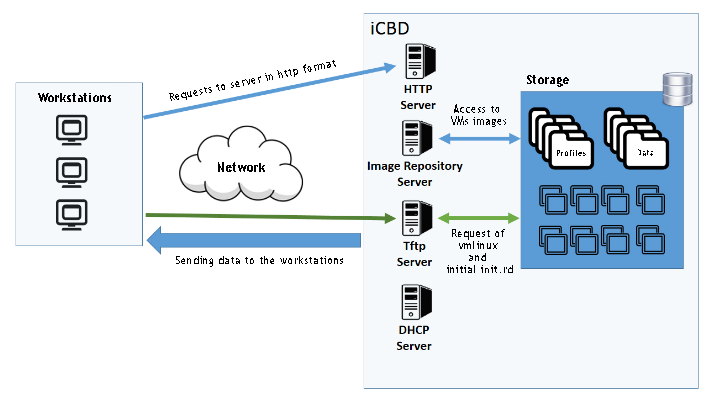
\includegraphics[height=3in]{cap1_icbd}
%    \caption{iCBD architecture. Adapted from \enquote{Linked clones baseados em funcionalidades de snapshot do sistema de ficheiros} by Nuno Alves~\cite{Nuno2016}}
%    \label{fig:icbd}
%\end{figure}

%\newpage

It is also interesting to briefly discuss some of the primary objectives of the project, being:
\begin{itemize}
    \item Offer a work environment and experience of use so close to the traditional one that there is no disruption for the users when they begin to use this platform.
    %
    \item Enable centralised management of the entire infrastructure including servers in their multiple roles, storage and network devices from a single point.
    %
    \item Complete decoupling between users and workstations in order to promote mobility.
    %
    \item Support the disconnected operation of mobile workstations.
\end{itemize}

With all the above in account, there is a clear separation from other solutions previously and currently available. As far as we know, no other solution is so comprehensive in the use of the resources offered by workstations whether they are PCs, laptops or similar devices.
\newpage


%%-------------------------------------------------------------------
%%	1.3. - Previous Work
%%-------------------------------------------------------------------
\subsection{Previous Work} % (fold)
\label{sub:previous_work}

There have previously been two dissertations involved in this project. The work of those students has centred in the creation of the instances of virtual machines, more specifically in a creation supported by native snapshot mechanisms of the file system where the templates reside. Testing several Files Systems that present the requirements mentioned above. As well as, conduct an analysis on the performance of those systems when working with a typical load for the platform. 
In a few words, the work opens a path where the snapshots stop being tied to the hypervisor as a tool for the provisioning (thin or full) of clones and bestowing the job to the file system snapshot system, which is fundamental to deliver a centralised management solution.
As is happening presently, the two theses have followed two different paths in an attempt to determine which type of file system best suits these objectives. 
In that sense, one of the works was used a local file system, named BTRFS, as the other followed the object-based storage path, adopting the CephFS.



%%-------------------------------------------------------------------
%%	1.4 - Problem Stating and Main Contributions
%%-------------------------------------------------------------------
%\section{Problem Stating and Main Contributions} % (fold)
\section{Problem Stating and Main Contributions}
\label{sec:project_contributions}

This dissertation aims to build upon the previous contributions, deeply study the core of the iCBD platform and tackle the next set of questions, mainly:

\begin{itemize}
	%\item \textit{Needing a distribute data model between nodes, which can be set apart geographically, how to achieve that and maintain the consistency and availability of the data?}
	%\item \textit{How to scale the platform in order to handle a large number of clients and maintain or even enhance the performance?}
	\item \textit{In a geographically dispersed, multi-server iCBD infrastructure, how do we keep the VM templates consistent and available even on the presence of network faults?}
	%
	\item \textit{How do we keep the management of templates across multiple "zones", simple?}
	%
	\item \textit{How to scale the platform in order to handle a large number of clients and maintain or even enhance its performance?}
\end{itemize}




%%-------------------------------------------------------------------
%%	3.2. - Replication and Caching - The Problem 
%%-------------------------------------------------------------------
\subsection{Replication and Caching - The Problem}
\label{sec:replication_cache_theproblem}

To answer these questions, we can formulate small topics that guide the work in a more focused way creating a list of general requirements to be addressed by this thesis.
In general, the work will be divided into two major subjects, were the second is a direct consequence and requires the first.


%\subsection{Motivation and Goals}
\paragraph{Motivation and Goals}
\label{par:motivation_goals}

Providing a mechanism that ensures the correct replication of data between nodes of the platform is paramount. This process also needs to confer other properties such as achieving the best performance on data transferences, being in a factor of speed or the used bandwidth. Another point of interest is the fact that the replication process should easily integrate with any File System used in the Storage Layer (taking into account that is fundamental that the file system provides some variety of snapshotting mechanism) trying not to add a sizeable computational load.
Following this idea, we may start thinking on how to deliver to the clients the benefits of replicating data. The replication procedure is not only a useful tool to propagate efficiently data changes throwout the nodes of the platform and act as insurance from a data loss disaster, but also capitalise on getting closer to the clients the resources that they need. Following this line of thought, an answer to the second question starts to appear. It is not only necessary to think about the location of the data, but also to study which services are used by the platform that are fundamental for running images on the client's workstations and how to integrate all so as to deliver the best experience to the highest number of clients.
To summarise, the following list poses the key requirements had in mind during the planning and execution of this effort:

\begin{itemize}
    \item The iCBD platform needs to be always available and maintain top-notch performance in multiple locations while serving a considerable number of clients.
    %
    \item Produce a mechanism that allows the replication of data not only for security reasons (backup) but also providing that data closer to the client.
    %
    \item With the data near its consumer study what is required to deliver that data to the client in the most efficient way.
	%
	\item Boot a client with the minimal number of the platform functionalities possible, simplifying the processes near the consumer.
\end{itemize}

%\subsection{System Overview}
%\label{sub:system_overview}

%\subsection{Requirements}
%\label{sub:requirements}



%%-------------------------------------------------------------------
%%	1.3. - Main Expected Contributions
%%-------------------------------------------------------------------
\subsection{Main Expected Contributions} % (fold)
\label{sub:main_expected_contributions}

The main expected contributions are: 

\begin{itemize}
  \item Perform a throughout analysis of the already implemented iCBD platform modules and the several layers where it expands in order to understand the inner works, providing an excellent platform to build upon and allowing for an efficient planning of the remaining work. 
  %
  \item The study, develop, and evaluate an implementation of a distributed and replicated BTRFS file system for VM storage.
  %
  \item Implement a client-side caching solution in order to increase availability, improve response time, and enable better management of resources.
  %
  \item Integrate the solutions described above  with the work previously developed and the existing infrastructure
  %
  \item And finally, carry out a series of tests that lead to a meaningful conclusion and that provide help in the design of the remaining platform.
\end{itemize}


In a more concrete approach, we present the work plan, for achieving the above objectives, distributed by the two main topics.


%\subsubsection{Replication}
\paragraph{Replication}
\label{par:replication_goals}

\begin{itemize}
	\item Create a middleware that integrates with the core functionalities already developed within the iCBD platform.
	%
	\item Should aim to be storage provider agnostic (in this thesis work with BTRFS but remain easy to integrate with others).
	%
	\item Work with compression algorithms to achieve a lower bandwidth consumption.
	%
	\item Be able to use encrypted and unencrypted communications for all data flows. 
	%
	\item Capitalize the snapshotting features of the storage layer in order to minimise the volume of data transferred, only sending the differences between versions whenever possible.
	%
	\item Provide a simple CLI and a REST API for interacting with the replication module functions.
\end{itemize}


%\subsubsection{Cache Server}
\paragraph{Caching}
\label{par:caching_goals}

\begin{itemize}
	\item Dilute some cost of the infrastructure by having commodity hardware as proximity servers.
	%
	\item Bring the data closer to the final clients giving enough storage capacity to servers, storing the most used images.
	%
	\item Facilitate a user experience where the is no distinction on booting an OS from a local disk or the iCBD platform.
	%
	\item Build a completing working iCBD platform on the FCT NOVA campus.
	%
	\item Study the benefits of introducing cache servers and the platform performance as a whole, comparing the performance of the system to a traditional OS install base.  
\end{itemize}

A detailed view of the work conducted is presented in \textbf{Chapter~\ref{cha:impl_replication_caching}}.
% subsection main_expected_contributions (end)



%%-------------------------------------------------------------------
%%	1.5 - Document Structure
%%-------------------------------------------------------------------
\section{Document Structure} % (fold)
\label{sec:document_structure}

The remnant document is structured as follows: 

\begin{itemize}

  \item \textit{Chapter~\ref{cha:research_context}}  \textbf{Research Context} - This section presents existing technologies and theoretical approaches which were the target of study, such as, storage systems and several of its features, as well as several intrinsic characteristics of virtualisation techniques.
	%
  \item \textit{Chapter~\ref{cha:icbd}} \textbf{iCBD - Infrastructure for Client-Based Desktop} - In this chapter, there is a presentation of the iCBD platform as a whole. Giving also an overview of the solution with its multiple layers and trying to explain the conceptual and architectural decisions made, being essential to understanding the bigger picture and where the remaining work fits in.
  %
  \item \textit{Chapter~\ref{cha:impl_replication_caching}} \textbf{Implementation of the \textit{iCBD-Replication and Cache Server}} - Starts giving an in-depth view of the implementation of the iCBD Replication module, detailing the architectural decisions and the implemented components. Then, follows a description on the efforts to build a test infrastructure on the FCT NOVA grounds, solely dedicated to the iCBD project. Concluding the chapter with an explanation on how to build and deploy an iCBD Cache Server node that can serve the entirety of workstations on a laboratory in the Computer Science Department.
  %
  \item \textit{Chapter~\ref{cha:evaluation}} \textbf{Evaluation} - The evaluation process employed in the validation of our implementation is presented in this chapter. Emphasizing the results of the work developed, analysing the results obtained and comparing with baseline values.
  %
  \item \textit{Chapter~\ref{cha:conclusion}} \textbf{Conclusions \& Future Work} - This last chapter concludes the dissertation by answering the questions stated in the Introduction, summarising the results achieved in the evaluation process and presents some improvements ideas that wore formulated during the implementation process and are believed to be a good starting point for future work.
\end{itemize}

% section document_structure (end)

%!TEX root = ../template.tex
%%%%%%%%%%%%%%%%%%%%%%%%%%%%%%%%%%%%%%%%%%%%%%%%%%%%%%%%%%%%%%%%%%%%
%% chapter2.tex
%% NOVA thesis document file
%%
%% Chapter with the template manual
%%%%%%%%%%%%%%%%%%%%%%%%%%%%%%%%%%%%%%%%%%%%%%%%%%%%%%%%%%%%%%%%%%%%

%%-------------------------------------------------------------------
%%	2 - iCBD - Infrastructure for Client-Based (Virtual) Desktop (Computing)
%%-------------------------------------------------------------------
\chapter{iCBD - Infrastructure for Client-Based Desktop}
\label{cha:icbd}

The acronym iCBD stands for Infrastructure for Client-Based (Virtual) Desktop (Computing). Is a platform being developed by an R\&D partnership between NOVA LINCS, the Computer Science research unit hosted at the Departamento de Informática of Faculdade de Ciências e Tecnologia of Universidade NOVA de Lisboa (DI-FCT NOVA) and SolidNetworks – Business Consulting, LDA part of the Reditus S.A. group. 
Where the primary goal is to achieve a particular kind of VDI infrastructure, a client based VDI, where client's computations are performed directly on the client hardware opposed to on big and expensive servers.

This chapter will address the central concepts and associated technologies encompassed in this project, particularly:

\begin{description}
	\item [Section~\ref{sec:virtualization}] overviews virtualization as a core concept and discuss in particular the data and metadata storage method.
	%
	\item [Section~\ref{sec:storage}] studies the principal characteristics of a file system, with emphasis on snapshot techniques and replication and consistency models.

\end{description}


%%-------------------------------------------------------------------
%%	2.1 - The Concept
%%-------------------------------------------------------------------
\section{The Concept} % (fold)
\label{sec:icbd_concept}


%%-------------------------------------------------------------------
%%	2.2 - The Architecture 
%%-------------------------------------------------------------------
\section{The Architecture} % (fold)
\label{sec:icbd_architecture}


%%-------------------------------------------------------------------
%%	2.2. - Boot Layer 
%%-------------------------------------------------------------------
\subsection{Boot Layer}
\label{sub:icbd_architecture_boot}

%%-------------------------------------------------------------------
%%	2.2. - Client Layer 
%%-------------------------------------------------------------------
\subsection{Client Layer}
\label{sub:icbd_architecture_client}

%%-------------------------------------------------------------------
%%	2.2. - Storage Layer 
%%-------------------------------------------------------------------
\subsection{Storage Layer}
\label{sub:icbd_architecture_storage}





 

%!TEX root = ../template.tex
%%%%%%%%%%%%%%%%%%%%%%%%%%%%%%%%%%%%%%%%%%%%%%%%%%%%%%%%%%%%%%%%%%%%
%% chapter3.tex
%% NOVA thesis document file
%%
%% Chapter with iCBD project
%%%%%%%%%%%%%%%%%%%%%%%%%%%%%%%%%%%%%%%%%%%%%%%%%%%%%%%%%%%%%%%%%%%%


%%-------------------------------------------------------------------
%%	3 - iCBD - Infrastructure for Client-Based (Virtual) Desktop (Computing)
%%-------------------------------------------------------------------
\chapter{iCBD - Infrastructure for Client-Based Desktop}
\label{cha:icbd}

The acronym \gls{iCBD} stands for Infrastructure for Client-Based (Virtual) Desktop (Computing). Is a platform being developed by an R\&D partnership between \textit{NOVA LINCS}, the Computer Science research unit hosted at the \textit{Departamento de Informática of Faculdade de Ciências e Tecnologia of Universidade NOVA de Lisboa} (DI-FCT NOVA) and \textit{SolidNetworks – Business Consulting, Lda} part of the \textit{Reditus S.A.} group. 

The primary goal is to implement a client based VDI, a specialised form of \gls{VDI} infrastructure, where client's computations are performed directly on the client hardware as opposed to performed on big and expensive servers. With the distinctive characteristic of not having the necessity of investing in hard disks for the client devices, as well as hoping to solve prominent predicaments in the administration and management of large-scale computer infrastructure.

This chapter will address the central concepts and associated technologies encompassed in this project, particularly:

\begin{description}
	%
	\item [Section~\ref{sec:icbd_concept}] overviews the core concepts of the project and particularly note the limitations and peculiarities of current implementations in contrast with the chosen approach.
	%
	\item [Section~\ref{sec:icbd_architecture}] studies the main architectural components of the platform, with emphasis on the different layers and how  they act together to serve the end-user.
\end{description}
\newpage


%%-------------------------------------------------------------------
%%	3.1 - The Concept
%%-------------------------------------------------------------------
\section{The Concept} % (fold)
\label{sec:icbd_concept}

The iCBD as a project aims to investigate an architecture that leads to the development of a platform that is similar to a client-based VDI, while maintaining all the benefits of both client-based and server-based VDI. Additionally, it should present the power of working as a Cloud \gls{DaaS} without any of the bad traits of the approaches as mentioned earlier.

The aim is to preserve the convenience and simplicity of a fully centralised management platform for Linux and Windows desktops, instantiating those in the users physical workstation from virtual machine templates (VMs) kept in repositories. We will further address this subject in section \ref{sec:icbd_architecture}\\

To summarise the platform should be able to:

\begin{itemize}
	\item Adapting to a wide range of server configurations, without prejudice to the defined architecture.
	%
	\item Minimize disruption in the use of workstations for end-users, offering a work environment and experience of use so close to the traditional one, that they should not be able to tell it from a standard local install.
	%
	\item Simplify installation, maintenance and platform management tasks for the entire infrastructure, including servers in their multiple roles, storage and network devices, all from a single point of administration.
	%
	\item Allow for a highly competitive per workstation cost.
	%
	\item Maintain an inter-site solution to efficiently support, e.g., a geographically disperse multi-site organisation.
\end{itemize}


%%-------------------------------------------------------------------
%%	3.2 - The Architecture 
%%-------------------------------------------------------------------
\section{The Architecture} % (fold)
\label{sec:icbd_architecture}

%Topics:
%Introduce the layers
%Draw a diagram 
%Layers are a kind of role, not a single a defined service but a collection 

The iCBD platform encompasses the use of multiple services. To achieve a better understanding of its inner workings, we can group these services in four major architectural blocks as seen in  figure~\ref{fig:icbd_layers}.


\begin{figure}[htbp]
	\centering
	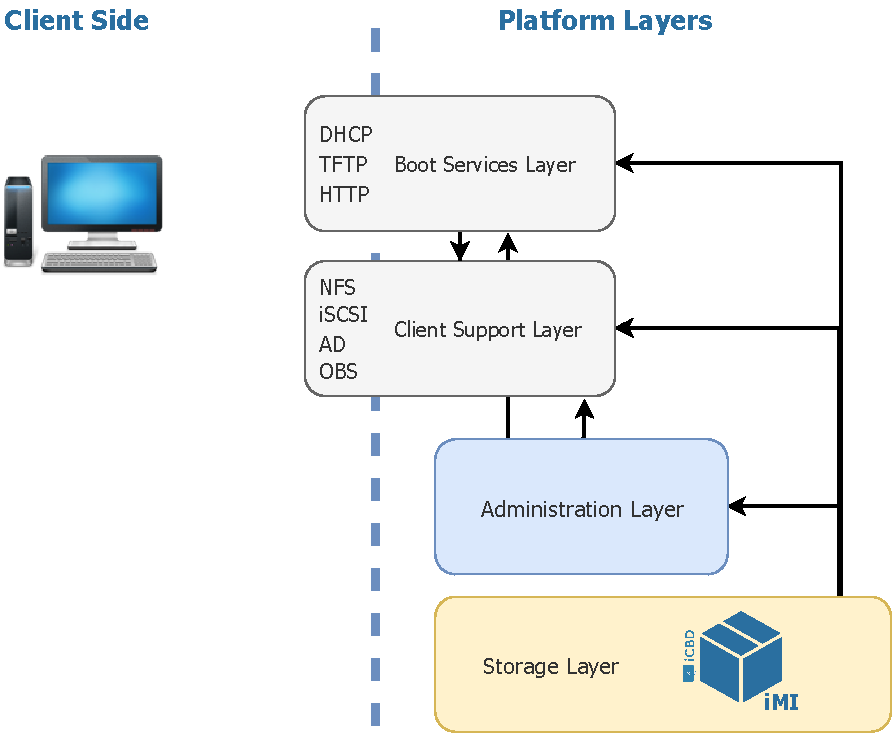
\includegraphics[height=4in]{cap3_iCBD_Layers}
	\caption{iCBD Layers View}
	\label{fig:icbd_layers}
\end{figure}


\begin{description}
	\item [\acrfull{iMI}] embodies the required files to run a iCBD platform client; this nomenclature was borrowed and adapted from Amazon Web Services AMI~\cite{aws_ami}. An iMI includes a VM template (with an operating system, configurations and applications), the iCBD boot package ( a collection of files needed for a network boot and custom-made to the operating system) and an assortment of configurations for services like PXE and iSCSI.
	%
	\item [Boot Services Layer] is responsible for providing the initial process from which the client machines will boot from the network, and later on transfer a bespoke boot package, using services such as \acrshort{PXE}, \acrshort{DHCP}, \acrshort{TFTP} and \acrshort{HTTP}.
	%
	\item [Administration Layer] to maintain all the iMI life cycle, from its creation to its retirement, currently this is done with a custom set of scripts.
	% takes advantage of a virtualisation stack (can be based in either \acrshort{KVM} or VMWare products) to engage in maintaining all the needed aspects for the successful creation and update processes of an \acrshort{iMI} lifecycle.  Employing a custom set of scripts, the creation of an iCBD Boot Package is also a duty of this layer. 
	%
	\item [Client Support Layer] provides support for client side operations including, e.g., authentication, read/write storage space for the client (since iMIs run on "diskless" workstations) and its home directories. 
	%deals with the demands of a deployed and running iCBD image, such as, providing read/write space (since iMIs run on diskless workstations) and storing users home directories. As well as, hosting domain controllers, centralised authentication amongst other services that can be already in place in the midst of a clients infrastructure. Granting the ability to deploy a customised iMI in any scenario.
	%
	\item [Storage Layer] maintains the repository of iMIs and provides essential operations such as version control of the VM images files. Our work is fundamentally focused on this layer, extending it in such a way that a single repository abstraction is built on top of the local / individual repositories through replication and caching. These local repositories are implemented on BTRFS or CEPH and may be exported to clients using \acrshort{NFS} or \acrshort{iSCSI}.
	
	%Is also in this layer that we seize the potential of replication features provided by the file systems employed. In this project, the storage relies on two mainstream file systems: BTRFS and CEPH. Together with services like \acrshort{NFS} and \acrshort{iSCSI} enables a way to export data to clients.
\end{description}
 
In the next subsections we will provide a more detailed description of each of the above-mentioned layers.

%%-------------------------------------------------------------------
%%	3.2. - iCBD Machine Image 
%%-------------------------------------------------------------------
\subsection{iCBD Machine Image}
\label{sub:icbd_imi}

\begin{figure}[htbp]
	\centering
	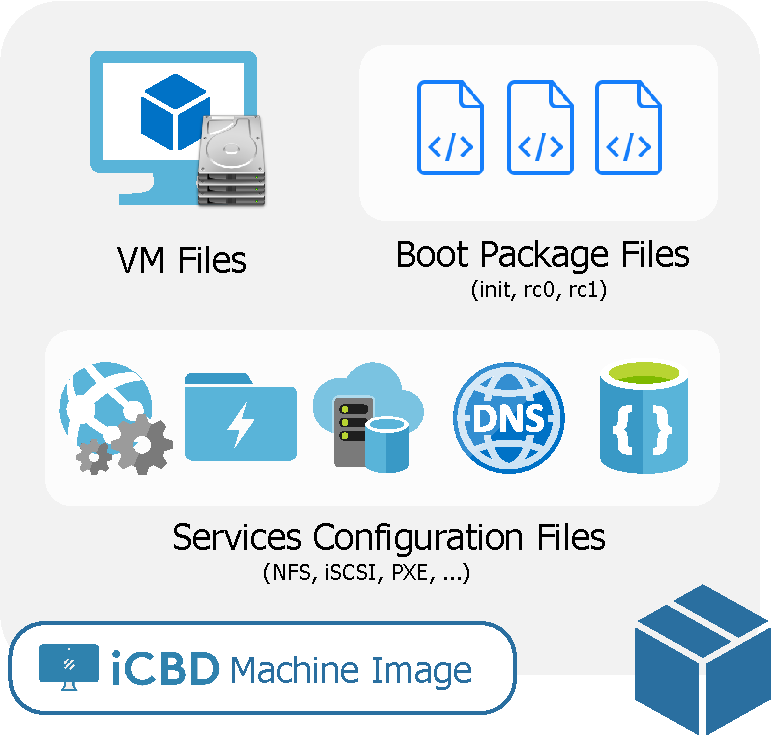
\includegraphics[height=4in]{cap3_iMI}
	\caption{iCBD Machine Image Files}
	\label{fig:icbd_iMI_files}
\end{figure}

In its essence, an iCBD Machine Image is the aggregation of everything that is needed to run an Operating System within the iCBD platform - data and configuration files. For the sake of simplicity, we categorise the files in three main groups.

\begin{description}
	\item [VM Template files] The main component is the virtual machine template in the form of a read-only image. As described in section~\ref{sub:res_vm_storage} the anatomy of a template follows the standard VMware and KVM formats either with multiple files (i.e., Virtual Disk Files like \texttt{.vmdk} or \texttt{.qcow}) or a \textit{raw} storage format.
	%
	\item [iCBD Boot Package files] In a network boot environment, such as the one used, there is a need to keep a set of files that manage the boot process of a workstation; these files can be included in the initial \textit{ramdisk} or later transferred over HTTP when needed. Included are an init file and at least two Run Control Script files (\texttt{rc0} and \texttt{rc1}) that are responsible for starting network services, mount all file systems and ultimately bring the system up in to the single-user level. With a tool such as \textit{BusyBox} (a single executable file with a stripped-down set of tools), a basic \textit{shell} is available during the boot process to fulfil all the required steps.
	%
	\item [Service Configuration files] Among the services that support iCBD, some do need changes in the configuration files. As an example, the "NFS exports" configuration file should reflect which file systems are exported, which networks a remote host can use, as well as a myriad of options that NFS allows to be set. The same happens to iSCSI, where an iSCSI target needs to refer to a backing store for the storage resource where the image resides. 
\end{description}

%\subsubsection{iMI Life Cycle}
\paragraph{iMI Life Cycle}
\label{subsub:icbd_imi_lifecycle}
The life cycle of an iMI encompasses all stages that take it throughout its course within the platform, Figure~\ref{fig:icbd_iMI_lifecycle} shows the major ones. From creation, through live deployment in use by multiple clients, and finally its decommission and placement in to temporary or cold storage.

\begin{figure}[htbp]
	\centering
	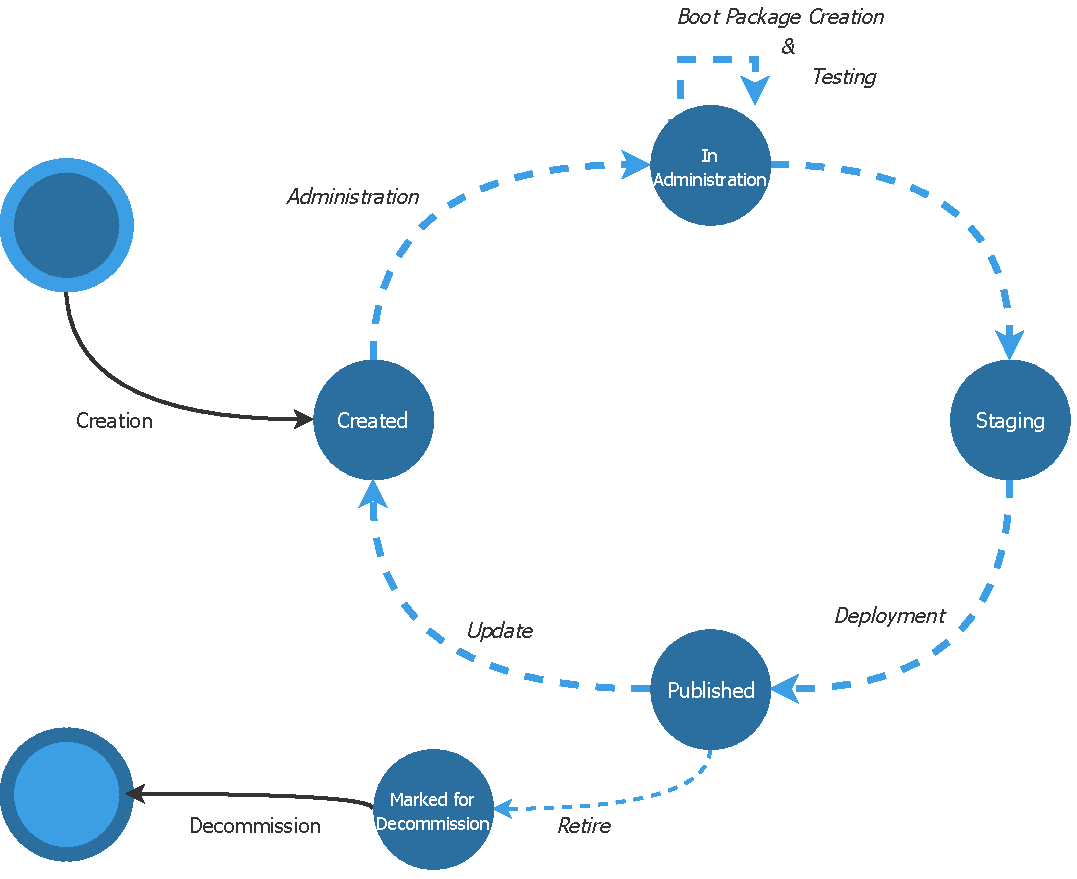
\includegraphics[height=4in]{cap3_iMI_Lifecycle}
	\caption{iMI Life Cycle inside the iCBD Platform}
	\label{fig:icbd_iMI_lifecycle}
\end{figure}

Each lap in the cycle is considered a new version. So every new update made to an iMI will spawn a new version. Through the snapshotting features of the storage layer, the creation of a new version is a rather straightforward and a computationally light operation.

During its life in the platform, an iMI can present it self into four main states:

\begin{description}
	\item [Created] After being inserted into the platform, an image is not instantaneously  ready to be served to clients and booted in a workstation; it must pass through a number of administration steps for the generation of a boot package.
	%
	\item [In Administration] An iMI goes through this phase in two moments: the first one, described above, where an image has just been injected into the platform. And the second and most frequent case, where an image needs to be updated or any way modified. 
	%It is here in this state that in interaction with the administration layer provides with a way to administer and update an iMI. 
	The iMI will stay in this state as long as it is being managed (which can take from a few minutes to hours). At the end this process the boot package is automatically created.
	% TODO Cap3 - FICAMOS AQUI NA REVISAO
	\item [Not Published] This status symbolises that the image is ready to work but isn't yet published and so not visible to platform users. This phase holds a particular interest in the testing the iMI for the correctness in the boot process and to ensure that the modifications were applied. Only after the testing procedures should an iMI made available for general use.
	%
	\item [Published] The stage where the iMI is expected to spend most of its time. One can think o   f this state as the proceeding into production of an iMI. After all the previous steps it is anticipated that the image is entirely ready to be delivered to the clients. At this stage, the platform in its Boot Services Layer announces to clients the possibility of choosing this image and provides the necessary support to its execution. Clients can instantiate the iMI as they please, taking advantage of the fact that can access their data and applications from nearly any device.
\end{description}

When an iMI completes a cycle and undergoes an update process, the old version is retired and goes to a fifth state, denominated \textbf{Marked for Decommission}, which is comparable to a stay in limbo. First, because when the administration process has initiated the probability of having clients using the image is significant, therefore the iMI needs to continue available for those clients. Even when the administration process ends, some client may still be using the image's old version. Thus only after all the clients cease utilising the iMI, can the image be transferred to its final state - \textbf{Decommission}. At this point, the version can be removed entirely from the platform or more wisely stored as a backup for some eventual failure in the future, or even if the administrator wants to recover an older state of the image.






%%-------------------------------------------------------------------
%%	3.2. - Boot Layer 
%%-------------------------------------------------------------------
\subsection{Boot Services Layer}
\label{sub:icbd_boot_layer}
% https://opensource.com/article/18/1/analyzing-linux-boot-process
% https://www.ibm.com/developerworks/library/l-linuxboot/index.html
% https://utcc.utoronto.ca/~cks/space/blog/linux/LinuxBootOverview?

From an end-user perspective, the only layer that is visible and interactive is the boot layer. The interface is lean and provides a way to select the image to boot in the workstation, however not every single aspect is noticeable. In the background, there is a need to resort to multiple services for starting a client's workstation with an iCBD Machine Image.

The platform provides two processes to remote boot an iMI. One instantiates, from an iMI, the Operating System natively on the bare metal workstation in the fashion of a standard diskless network boot. The other uses the above mechanism for provisioning a minimal iMI that was a hypervisor installed and virtualises any other iMI available in the storage layer. Both approaches are entirely transparent to the final user that does not grasp the differences and doesn't know if the working OS is virtualised or running natively.

The first part of the boot process starts like any other network boot, where a series of DHCP requests are used to provide the suitable client network parameters and particularly the location (IP address) of the TFTP server. Then begins the transference of a small network boot manager program. In this traditional PXE boot environment, a friendly looking tailored made graphical menu displays to the user an assortment of choices that announce the different iMIs ready to boot.

%\subsubsection{Booting an iMI in a Workstation }
\paragraph{Booting an iMI in a Workstation}
\label{subsub:icbd_booting_imi}
%(REF https://www.ibm.com/developerworks/library/l-initrd/index.html)
After the selection of an iMI in the PXE boot menu~\cite{ibm_linux_boot} the second-stage boot kicks in. Using \textit{PXELINUX} as a bootloader there is the capability of transferring a compressed Linux Kernal (vmlinuz) and an initial ramdisk (initrd) (REF in comment)through either TFTP or HTTP, is also in this step that some parameters needed during the boot are set with the correct values according to the image picked. After everything loaded into memory, the stage 2 boot loader invokes the kernel image, and after booted and initialised, the kernel starts the first user-space application. 

Commonly the first application is called init, and in the particular case of this platform, the init file starts the chain execution of other custom files (\texttt{rc0} and \texttt{rc1}). Those Run Control scripts configure every single aspect in the Operating System according to the characteristics of physical machine booting. The first step is to reconfigure the network card and obtain connectivity. Then, is determined if there is the need for getting more files indispensable for the remaining boot process if this need exists, then the missing files are transferred. The next script, \texttt{rc0}, deals with data volumes and their mounting method (i.e. r/w space, users home directories); in case of using the loading OS as a base for another iMI in virtualisation, some configurations are anticipated and applied. The file system of the underlying iMI is checked to verify if happens to be BTRFS or any other, in the case where BTRFS is adopted the Seeding capability comes into play in this step. After every aspect from the configuration is setup the \texttt{switch root} command is deployed moving the already mounted \texttt{/proc}, \texttt{/dev}, \texttt{/sys}, \texttt{/tmp} and \texttt{/run} to new root and makes this the new root filesystem.

At last, the residual configuration entails the update of the correct time with the NTP service and some last logging of statistics such as the elapsed time of the boot process and the bandwidth used by the sum of all operations.



%%-------------------------------------------------------------------
%%	3.2. - Administration Layer 
%%-------------------------------------------------------------------
\subsection{Administration Layer}
\label{sub:icbd_adm_layer}

One of the most important features provided by the platform, and personified in this next layer, is the ability to perform administration operations on an iMI. That task becomes simplified by the use of a provided image administration tool. Armed with such a mechanism any systems administrator in an organisation can make the changes that understand necessary (stuff like Operating System and software in general updates, add new software, modify configurations) and then publish the image in the platform for widespread use. 

%\subsubsection{The Administration Process}
%\label{subsub:admin_imi}

%\textbf{The Administration Process}
\paragraph{The Administration Process}
\label{par:admin_imi}
The administration tool consists of a series of scripts triggered by the main one called \texttt{adm}. Calling this script with the name of one iMI sets off the startup of a VM in a VMware ESXi server with a base image that will support the administration process. Commonly the OS used will be some flavour of Linux (Fedora 27, CentOS 7 or even Ubuntu 16.04 LTS).

The whole process makes extensive use of the snapshotting capabilities of the Storage Layer (whether using BTRFS or CEPH), with no prejudice to the complete system performance. For each iMI, there is a snapshot with an index number that relates to its version and age (i.e. the higher the number the most recent the version is). Multiple versions of an iMI persist stored in directories named by the index of the version. So, is simple to create a new linked clone from the most recent version.

The administration VM, after its boot process, will start a hypervisor (VMware Workstation or KVM) that in turn will get a new linked clone of the most recent version of the iMI to administrate. In this sense, this process makes use of nested virtualisation to achieve its goal, which can result in some slowness (even considering the use of a Type 1 hypervisor), but in theory, all the operations to the new snapshot could be performed on a physical machine using only one level of virtualisation. 
%(ref: https://www.linux-kvm.org/images/3/33/02x03-NestedVirtualization.pdf)
In this step, the snapshot that is in the management process is in a working directory, a temporary storage area with a limited lifetime to the duration of the procedure. This method serves two proposes. First, all the clients that are using the latest version of the iMI can remain using it with an administrative process running in parallel. The second is the ability to quickly discard all the changes made in the working directory in case of unwanted changes.

Finishing the process, with all the desired actions performed in the iMI, the administrator gets to chose between saving the changes done or discarding them. When choosing to proceed with saving the new version of the image, a process starts by changing the working directory to a permanent one, through a new linked clone of the working snapshot but this time following the naming system so that the version number will name the directory.


%\subsubsection{Creating the boot package}
%\label{subsub:createboot_imi}

\paragraph{Creating the boot package}
\label{par:icbd_create_bootpack}
Even after all the process described above, the iMI is not ready to boot, being the next step the creation of the boot package. This phase is the responsibility of the \texttt{mki} script which can be called immediately at the end of the administration process by the texttt{adm} tool depending on the type of the iMI.
The procedure is different for each type of iMI (Windows or Linux), but with a set of steps in common, being that the Linux iMIs requires a particular number of customisations. The peculiarity of these requirement comes from the fact that Linux iMIs can run natively on a client workstation serving as host for other images. Which in turn entails the creation of custom \texttt{initramfs} and \texttt{vmlinuz} files, the addition of Kernel drivers and firmware, the tailor-making of Run Control Scriptfiles (rc0 and rc1) that start the network services with a configuration compatible with the platform and mount the correct remote file systems. In the end, is also added a script called \texttt{runvm}, that is instrumental in managing the launch of a virtualised iMI, as well as configure the hypervisor parameters to take the best advantage of the client hardware.
However, there is more to the \texttt{mki} script. For both flavours of the iMIs, the configurations of the \textit{iSCSI targets} need an update to reflect the new version of the iMI, with the same happening to the \textit{pxelinux} configuration that requires the new paths to the files served to the clients.


%%-------------------------------------------------------------------
%%	3.2. - Client Layer 
%%-------------------------------------------------------------------
\subsection{Client Support Layer}
\label{sub:icbd_client_support_layer}


%!!! \textbf{TODO} !!!
% TODO Cap3 - Client Support Layer

\textbf{TOPICS :}
\begin{itemize}
	\item Provide r/w space (for the duration of the session)
	\item Stores users directories (Home directory)
	\item Keep core services like DHCP, NTP, DNS, ...
	\item Integrate with external services such as Samba shares, LDAP, Active directory, ..
\end{itemize}


%%-------------------------------------------------------------------
%%	3.2. - Storage Layer 
%%-------------------------------------------------------------------
\subsection{Storage Layer}
\label{sub:icbd_storage_layer}

%!!! \textbf{TODO} !!!
% TODO Cap3 - Storage Layer

\textbf{TOPICS :}
\begin{itemize}
	\item Why btrfs? (Snapshots, seeding)
	\item How are files stored?
	\item The use of BTRFS multiple subvolumes for different parts of the platform.
	\item The use of cloning to save multiple versions of an iMI, giving the possibility to roll back unwanted changes.
	\item The need to replicate data - multiple locations and cache server (one of the focus of the thesis)
	\item Should be transparent the the remaining layers. As being develop in Joao's thesis the use of CEPH  should be used with little to none modifications to other layers. (Interfacing through NFS or iSCSI just like BTRFS)
\end{itemize}

%https://blogs.oracle.com/developers/save-disk-space-on-linux-by-cloning-files-on-btrfs-and-ocfs2-v2
%In this case the file system does not create a new link pointing to an existing inode, it rather creates a new inode that shares the same disk blocks as the original file. This means that this operation only works within the boundaries of the same file system or subvolume. The outcome looks very much like a copy of the source file, but the actual data blocks have not been duplicated. Due to the copy-on-write nature, a modification of any one of the files will not be visible in the other file. Note that this should not be confused with hard links – this web page provides a good explanation of the differences.

%For Btrfs, you can invoke this feature by using the cp(1) utility with the --reflink option, which was added to the GNU coreutils in version 7.5 (released in Aug. 2009):


%For each iMI, there is a snapshot with an index number that relates to its version and age (the higher the number the most recent the version is).
%Multiple versions of an iMI are stored in directories named by the index of the version. So, is simple to create a new linked clone from the most recent version 

%\textbf{TODO - Talk about btrfs seed}
%The importance of btrfs seeding relays on the fact that this feature alows for the multiple mounting operation of the same file system in read only mode. Thus allowing multiple clients to use the same image.. (Fulcral to the the platform)
%http://www.oracle.com/technetwork/articles/servers-storage-admin/advanced-btrfs-1734952.html 



%!TEX root = ../template.tex
%%%%%%%%%%%%%%%%%%%%%%%%%%%%%%%%%%%%%%%%%%%%%%%%%%%%%%%%%%%%%%%%%%%%
%% chapter4.tex
%% NOVA thesis document file
%%
%% Chapter with lots of dummy text
%%%%%%%%%%%%%%%%%%%%%%%%%%%%%%%%%%%%%%%%%%%%%%%%%%%%%%%%%%%%%%%%%%%%
\chapter{Implementation of the \textit{iCBD-Replication and Cache Server}}
\label{cha:impl_replication_caching}

%This chapter addresses the implementation of the central topics of this thesis, divided into two major fields.
%We first start with a section talking about the creation of a middleware system that provides replication features in an integrated way to the iCBD platform. While providing a detailed description of the concept and architectural model, as well as the implementation decisions, made along the accomplishment of this contribution.
%Next, we show the work done on improving the performance of the platform clients. Displaying how setting up a client-side caching system that stores images adjacent to the consumers obtain that sought enhancements. Concluding in exploring the challenges of recreating the complete platform in a new environment and implementing a real-world scenario at Nova University Computer Science department laboratories. This chapter is partitioned as follows :

%will at last state the problem and motivation for introduction replication techniques in the storage components of the platform. Moreover, the section prefaces the importance of the implementation of cache servers that hold part of the distribution burden and crucial for the support of an increased number of clients. 

This chapter is about the core of this thesis: the iCBD-Replication and Cache Server, a middleware
system that provides replication features in an integrated way to the iCBD platform. Naturally, the first subsection provides a detailed description of the motivation, architecture and design aspects while the second subsection concentrates on the implementation. Finally, the last subsection deals with the process of building the Replication and Cache Server: that is, how the modules are installed and deployed in an iCBD infrastructure.

% TODO Cap4 - Rever estes pontos
\begin{description}
	\item [Section~\ref{sec:impl_mot_sysarch}] begins by explaining the motivation for the implementation of a replication module within the iCBD platform, as well as explaining the need to include a new role in the platform with the creation and deployment of a cache server near the clients. Concluding with the overall architecture of the system and how both topics complement each other.
    %
    \item [Section~\ref{sec:impl_icbdrep}] overviews the implementation of the middleware dubbed iCBD-Replication. Beginning the journey through the initial architectural process and then showing the implemented components and their interaction with the several layers of the platform.
    %
    \item [Section~\ref{sec:impl_cache_server}] shows how the complete iCBD platform was installed in the NOVA University cluster. Then, a description of the work performed to include a client-side caching server directly connected to the final clients.
    %
\end{description}
\newpage

%%-------------------------------------------------------------------
%%	4 - Motivation and System Architecture
%%-------------------------------------------------------------------
\section{Motivation and System Architecture}
\label{sec:impl_mot_sysarch}

One of the key objectives of iCBD is to provide a platform that can stretch from a fully hosted, on-site architecture to one where an important part of its services is cloud-based. Naturally, in-the-middle solutions are also interesting, such as one where, e.g., both the administration and storage of \textit{“golden”} iMIs are cloud-based, while the rest is on-premises. Therefore, it becomes evident that data locality is an important subject, and thus one must study how data flows between the components of the iCBD platform – a complex, data-intensive platform, boasting multiple storage devices and many different networks, accessed by multiple consumers demanding data at any given time.

All these factors, allied to the desire of having a distributed and scalable platform architecture, result in the need to design a new service whose mission is to ensure that data is correctly replicated in the appropriate places, and consistency of the various versions of the iCBD Machine Images stored is maintained. This led to the high-level architecture of Figure~\ref{fig:impl_icbd_rep_arch_simple}

%\subsection{Motivation}
%\label{sub:impl_mot}

%\subsection{System Architecture}
%\label{sub:impl_sysarch}

\begin{figure}[htbp]
    \centering
    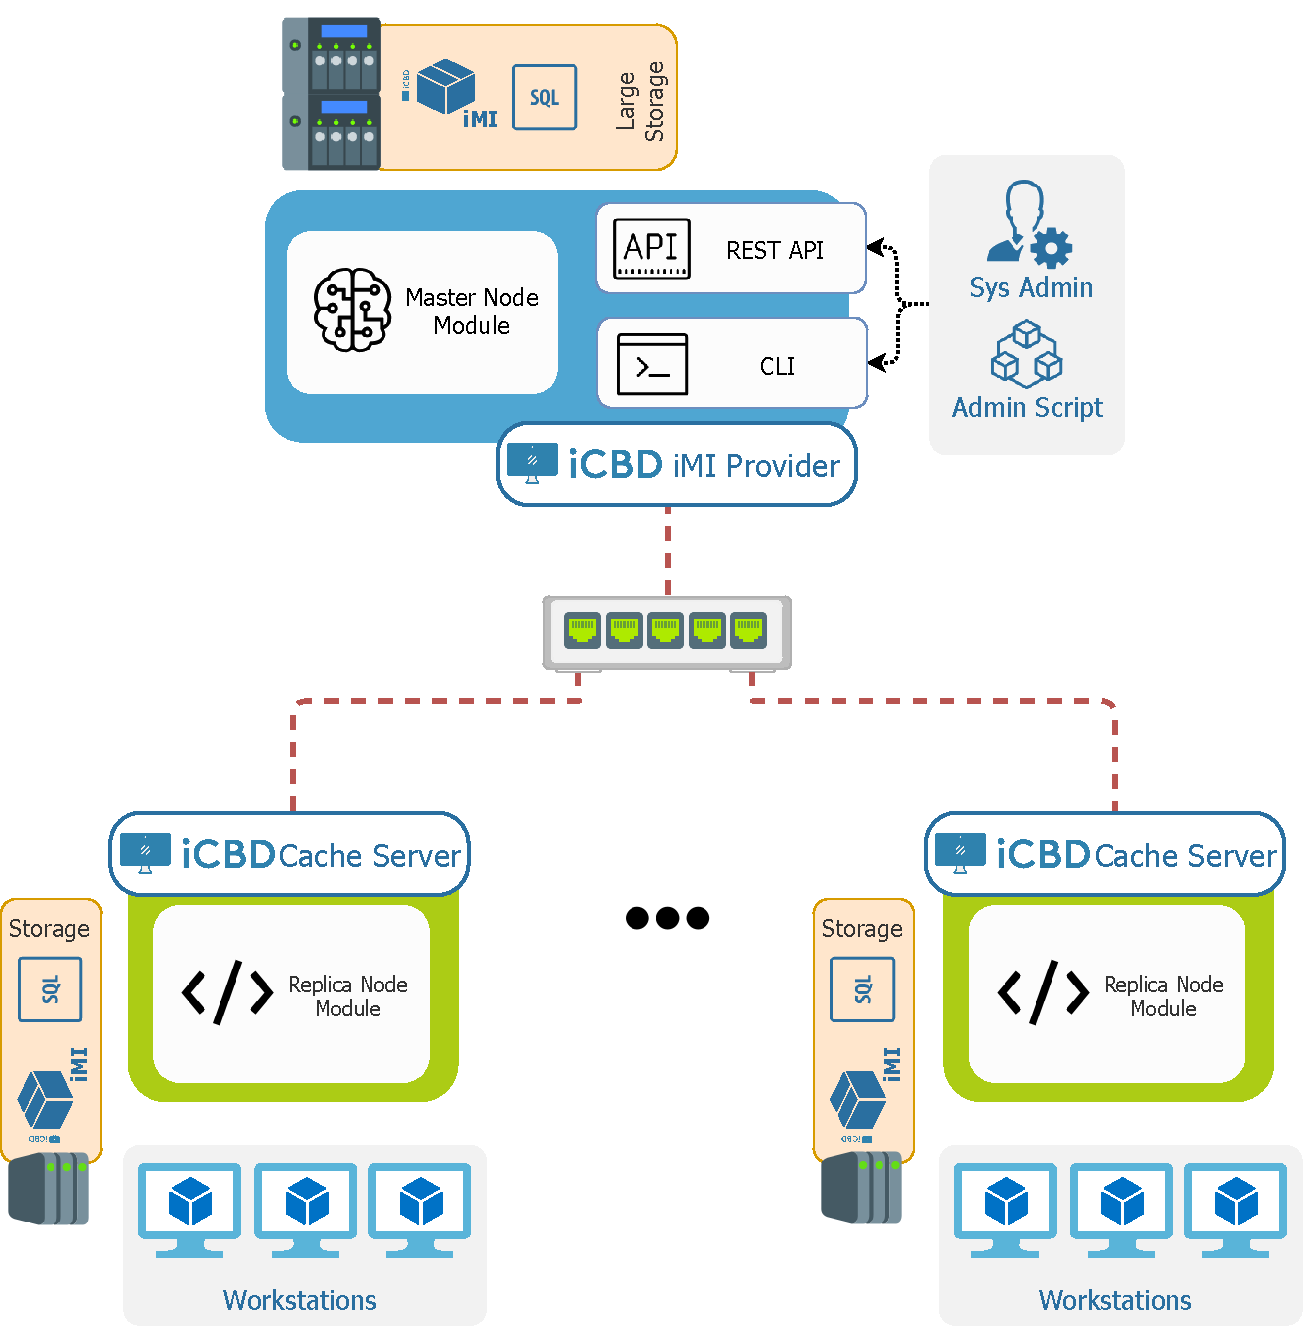
\includegraphics[
    height=13cm
    ]{cap4_icbd_rep_simple}
    \caption{iCBD Replication and Caching Architecture (high-level)}
    \label{fig:impl_icbd_rep_arch_simple}
\end{figure}

\pagebreak

%%-------------------------------------------------------------------
%%	4 - Implementation of a Replication Module
%%-------------------------------------------------------------------
\section{Implementation of a Replication Module}
\label{sec:impl_icbdrep}

%One of the central objectives of iCBD is to provide a platform that can be both cloud-centric, with the administration and a portion of the storage burden gathered in a public cloud, or fully hosted on client premises. Either way, it becomes evident that data locality is an important subject, which means that there is the necessity to study how this data will flow between the multiple components of the iCBD platform.
%As can be imagined, this is a data-intensive platform, boasting multiple storage devices in many networks and an array of consumers demanding that data at any given time.

%All these factors allied to the platform architecture result in the need to create a new component, whose chief mission is to ensure that the data is correctly replicated in the appropriate places, maintaining the consistency of the various versions of the iCBD Machine Images stored.

When our project started, iCBD was already available; therefore, our Replication and Caching Service (from now on, RCS) had to be integrated with the existing architecture and support (and enhance) the previous work. This influences the choices available for the RCS implementation and could, in a worst-case scenario, severely limit them. Fortunately, that was not the case.

iCBD was designed from the start based on the assumption that the storage layer where iMIs live was built on top of a storage system which supports snapshots. In the first prototype, Btrfs was chosen for the storage layer but, in theory, any storage system that supports snapshots can be used in the platform. That is, in fact, the case with a parallel work being developed in another dissertation, where the focus is the use of an object-based storage system, Ceph.


%%-------------------------------------------------------------------
%%	4. - Requirements of the Module
%%-------------------------------------------------------------------
\subsection{Requirements}
\label{sub:impl_requirements_icbdrep}

%\textbf{TOPICS :}
%The file system is set BTRFS will be used.
%Many reasons for that:
%The most important is the support for snapshots
%Compression

%Since the beginning of this work, the file system selected for use in the storage layer was selected, this is due to the fact that, there was already a functioning prototype of the core iCBD platform making use of BTRFS for all data storage matters. The most critical feature for the operation of the platform is that the file system supports snapshots. BTRFS is a modern file system based on the copy-on-write (COW) principle capable of creating lightweight copies of a file. We detailed the importance of this trait in Section~\ref{sub:icbd_storage_layer}.
 
%The condition described above applies only in the choice of the File System, in theory, any File System that supports snapshots can be employed in the platform. That is, in fact, the case with the work developed in a dissertation carried out in parallel to this one, where the focus is the use of an object-oriented file system, in particular, the CEPH File System.
%Due to this imposition, it is key that this work makes the best use of the BTRFS features, exploring the incremental backup capabilities. More, the replication process should fully integrate with the core platform that already distributes iMIs to clients. Preservation of consistency of the iMIs is also a concern, assuring the distribution of new versions when they are created.

%Moreover, it should be taken in account the locality of the data, since the communications could originate and end in the same data centre and the same local network, or happening between different locations that can be in opposite sides of the world. Such aspects as the bandwidth used and the encryption of the data becomes essential to address, requiring the examination of several compression algorithms that can be accommodated to the way the data is processed and also ways of keeping this data secure by encrypting the communications.

Btrfs is a modern file system based on the concept of copy-on-write (COW): it is capable of creating lightweight copies of filesystem structures – files, directories, volumes. We already detailed the importance of this trait in Section~\ref{sub:icbd_storage_layer}. Therefore, a mandatory step was to investigate Btrfs-provided tools that could help us to achieve our primary goal: being able to move information (“base” iMIs and their snapshots) around, from “master” to “secondary” nodes, while consuming the minimum bandwidth – one must not forget that, while a typical Linux iMI is less than 10 GB, a Windows 10 iMI is circa 40 GB. We found that Btrfs has incremental backup capabilities, and therefore we set out to explore those.
 
So,  Btrfs’s incremental backup capabilities are a good starting point; however, their purpose is to help in data transfer; but that is not enough. Preservation of consistency of the iMIs is also a concern, as one has to assure that iMIs cached in the RCSs are up-to-date, and when a new iMI is created its distribution will start “immediately”, to ensure high availability in case of faults. Moreover, the locality of the data should be taken into account, since data transfer endpoints may be located within the same data centre, or at, e.g., geographically disperse regions in the world. Bandwidth use and data encryption become essential, requiring the study of compression algorithms and encryption techniques.


%\subsubsection{Preliminary tests on the BTRFS Incremental Backup features}
\paragraph{Btrfs Incremental Backup feature}
\label{par:impl_incremental_btrfs}

%A first step is trying to understand the most efficient way to transfer this unique kind of data (i.e. an iMI). Given the fact that we are working with a file system with snapshots capabilities, we want to take advantage of this functionality and minimise the amount of data roaming the network.

%The BTRFS developers provide a userspace set of utilities that can manage BTRFS filesystems, called \texttt{btrfs-progs}. Within that set of tools, there is a pair of commands, \texttt{btrfs send}~\cite{btrfs_send}, and \texttt{btrfs receive}~\cite{btrfs_receive}, that provides the capability to transport data via a stream and employ those differences in a remote filesystem. 

%The send command facilitates the process of generating a stream of instructions that describe changes between two subvolume snapshots. Also available in the command is the ability to use an incremental mode, where given a parent snapshot that is available in both send and receive sides, only the small delta between snapshots (e.x. \textit{V2} and \textit{V2-1} in fig~\ref{fig:icbd_rep_imi_snap}) is going to integrate the stream. This feature is outstanding since considerably reduces the amount of information that needs to be transferred to reconstruct the snapshot in the receiving end. The send side operations occur in-kernel, beginning by determining differences within subvolumes and based on those differences the kernel generates a set of instructions in a custom formulated stream.

%On the remote end, the received command accepts the stream generated by the send command and uses that data to recreate one or more snapshots. Contrary to the send command, receive executes in user space, replaying the instructions that come in the stream one by one, these instructions include the most relevant calls found in a Virtual File System, with Unix system calls like \texttt{create()}, \texttt{mkdir()}, \texttt{link()}, \texttt{symlink()}, \texttt{rename()}, \texttt{unlink()}, \texttt{write()}, along with others.~\cite{btrfs_design}

A first step is trying to understand the most efficient way to transfer this unique kind of data (i.e. an iMI). Given the fact that we are working with a file system with snapshots capabilities, we want to take advantage of this functionality and minimise the amount of data roaming the network.

Btrfs has a set of userspace utilities to manage Btrfs filesystems, called \texttt{btrfs-progs}; these include a pair of commands, \texttt{btrfs send}~\cite{btrfs_send}, and \texttt{btrfs receive}~\cite{btrfs_receive}, that provide the capability to transport data via a stream and apply differences from/to a remote filesystem. The send command simplifies the process of generating a stream of instructions that describe changes between two subvolume snapshots. Also available is the ability to use an incremental mode, where given a parent snapshot that is available in both the send and receive sides, only the small delta between snapshots (e.x. V2 and V2-1 in Figure~\ref{fig:icbd_rep_imi_snap}) is going to integrate the stream. This feature considerably reduces the amount of information that needs to be transferred to reconstruct a snapshot in the receiving end. The send-side operations occur in-kernel, beginning by determining differences within subvolumes and, based on those differences, the kernel generates a set of instructions in a custom-formulated stream.

\begin{figure}[htbp]
    \centering
    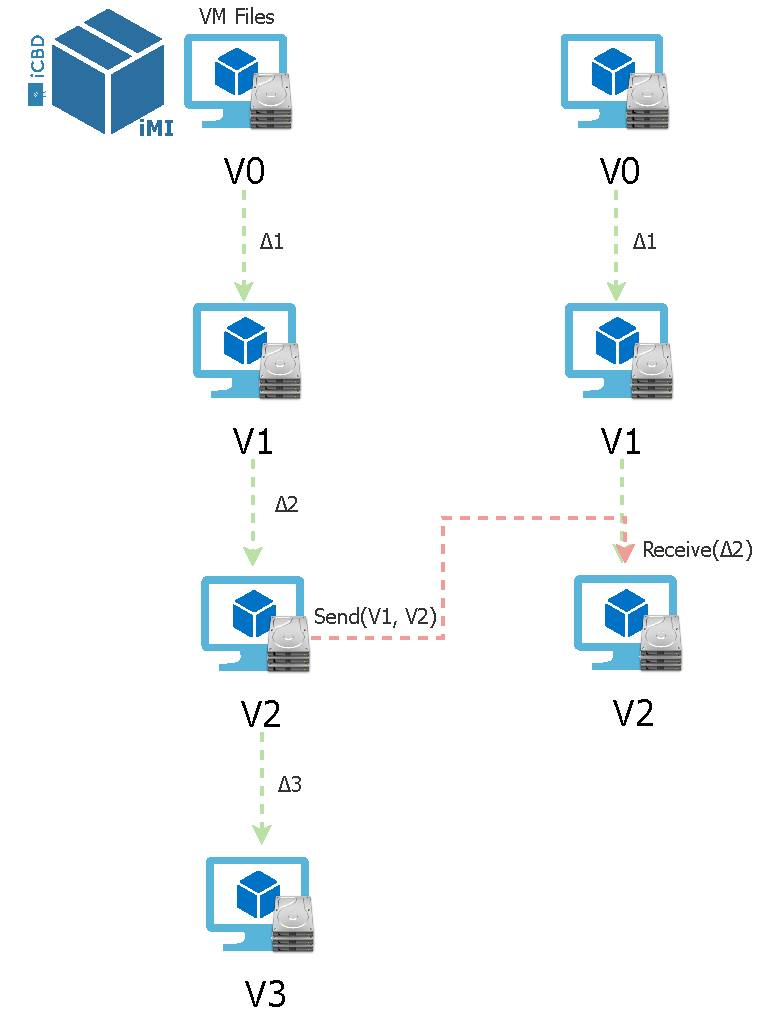
\includegraphics[
    	height=11cm
    ]{cap4_iMI_deltas}
    \caption{iCBD iMI Snapshots Structure}
    \label{fig:icbd_rep_imi_snap}
\end{figure}

On the remote end, the receiving command accepts the stream generated by the send and uses that data to recreate one or more snapshots. Contrary to the send command, receive executes in user space, replaying the instructions in the stream one by one; the set of instructions includes the most relevant calls found in a Virtual File System, such as \texttt{create()}, \texttt{mkdir()}, \texttt{link()}, \texttt{symlink()}, \texttt{rename()}, \texttt{unlink()}, and \texttt{write()}, along with others~\cite{btrfs_design}.


%https://btrfs.wiki.kernel.org/index.php/Incremental_Backup
%https://www.samba.org/ftp/rsync/rsync.html

\pagebreak

%%-------------------------------------------------------------------
%%	4. - System Overview
%%-------------------------------------------------------------------
\subsection{System Overview}
\label{sub:impl_system_overview}


\begin{figure}[htbp]
	\centering
%	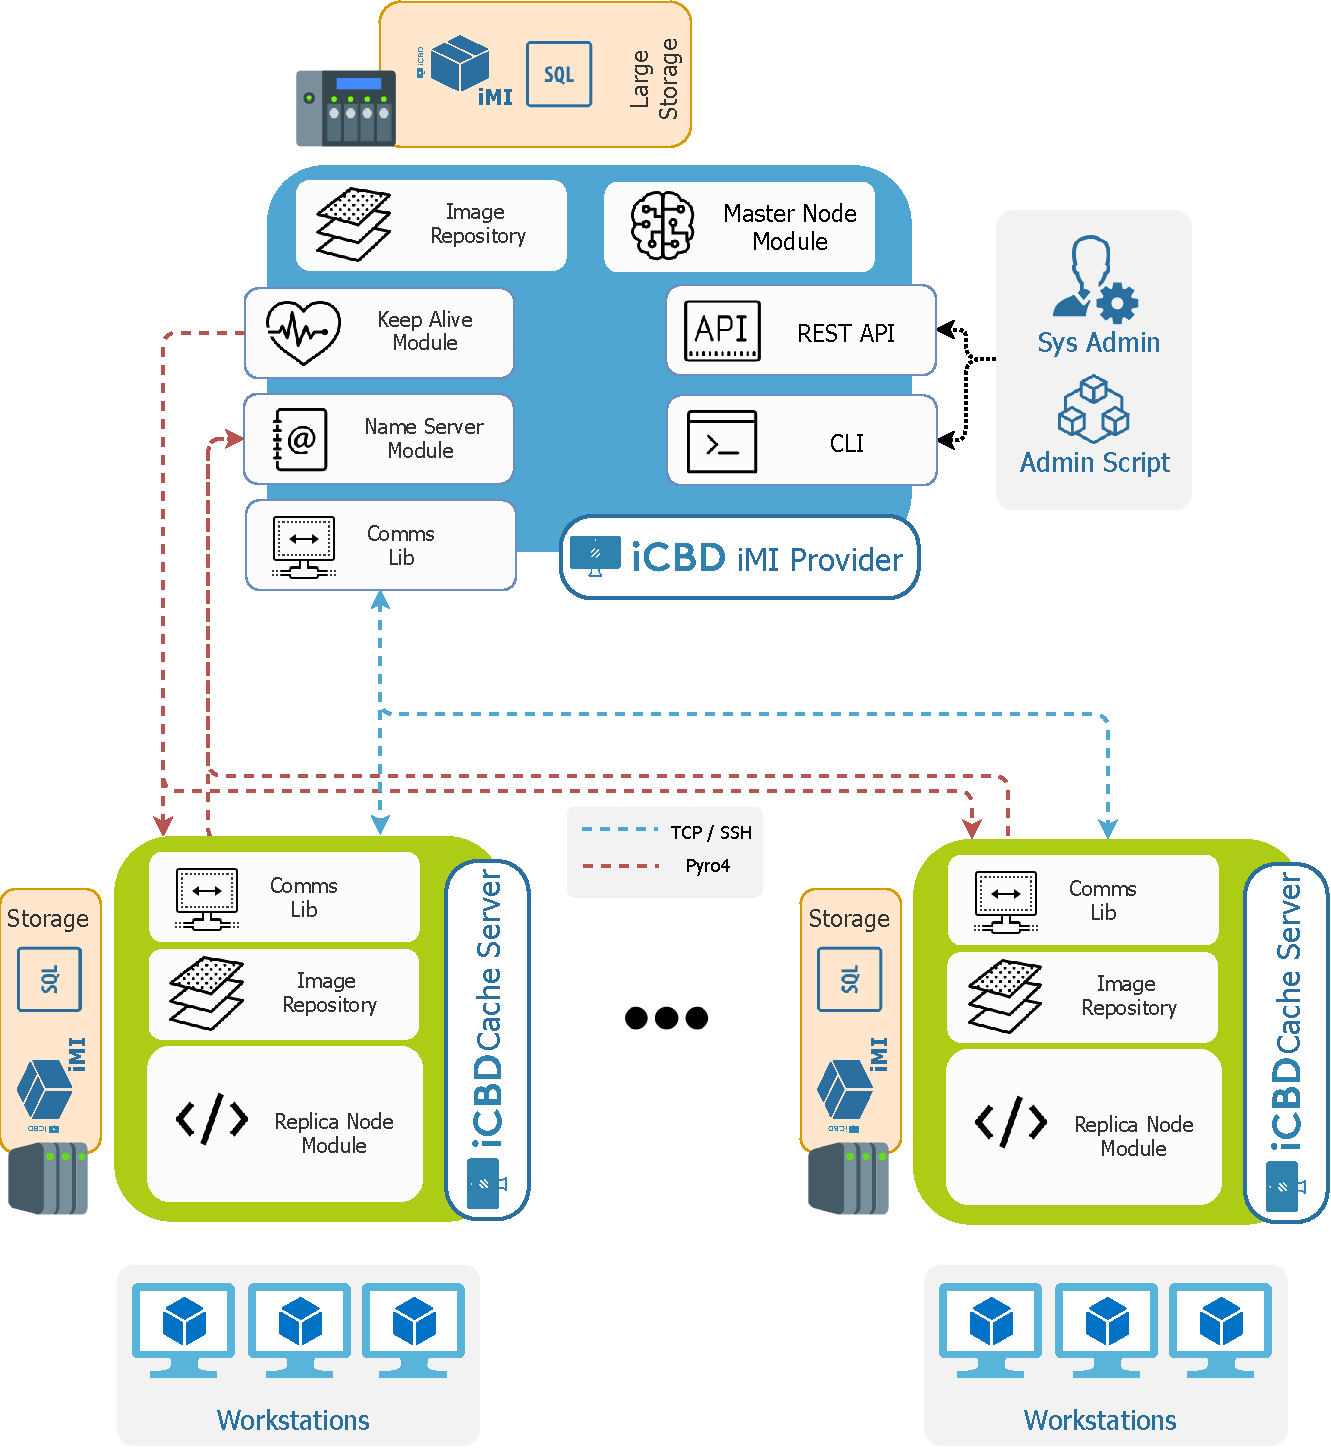
\includegraphics[height=4in, width=\textwidth]{cap4_icbd_arquit}
	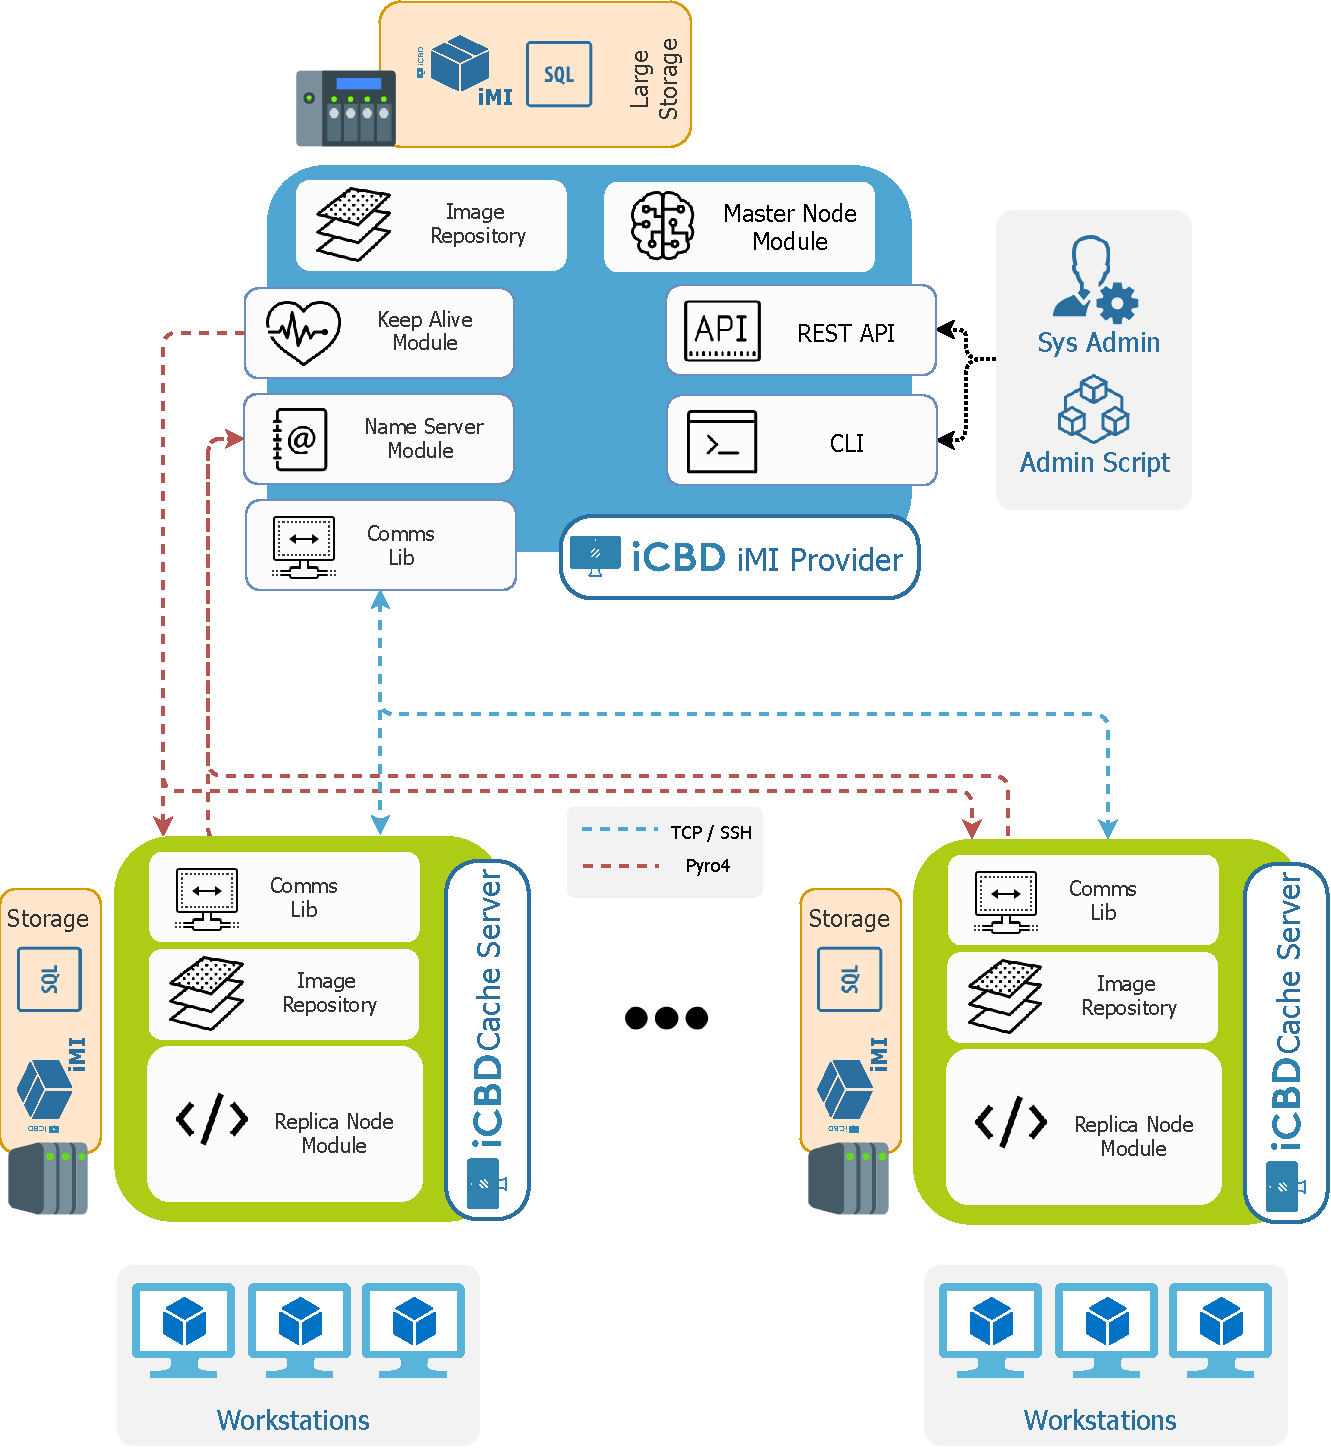
\includegraphics[width=\textwidth]{cap4_icbd_arquit}
	\caption{iCBD Replication Modules and Communications}
	\label{fig:icbd_rep_mods_comms}
\end{figure}
 
%Since the replication module needs to interact with several bash scripts, with the core iCBD platform, including command line tools and some operating systems low-level features, we betted that the most suitable approach was creating a python distributed middleware using a master-replica paradigm.

%Python as a programming language enjoys some valid idiosyncrasies, functioning as an object-oriented language, possessing an extensive standard library and enjoys a big community delivering packages with a wide range of functionality, all facts that contribute to make it the best programming language to bundle everything together.

%The several modules of the middleware comprise the main functionalities allowing a node to behave as a Master or Replica node, where each one maintains its individual Image Repository. Then there are also a number of libraries that were developed to interface with some tools, as the BTRFS tool talked about above~\ref{par:incremental_btrfs}, to interface with an SSH connection, build wrappers for compression algorithms and even provide a REST API.

%An overview with a small description of the functionality of each component of the system follows:

Since the replication module interacts with different tools and utilities, e.g., bash scripts and command line tools and some OS calls, we think that the most suitable approach was to create a Python distributed middleware layer using a master-replica paradigm.

Python, as a programming language, enjoys some idiosyncrasies, functioning as an object-oriented language, possessing an extensive standard library and enjoying a big community delivering packages with a wide range of functionality; all these facts contribute to make it the most appropriate programming language to bind everything together in our iCBD platform.

Our middleware is composed of several modules and includes all the necessary functionalities that allow a node to behave as a Master or as a Replica, where each maintains its individual Image Repository. A number of libraries were also developed: to interface with some tools, such as Btrfs send/receive and with SSH, to build wrappers for compression algorithms, and even to provide a REST API.

An overview with a small description of the functionality of each component of the RCS system, displayed in Figure~\ref{fig:icbd_rep_mods_comms}, follows:

\begin{description}
	\item [Master Node] This node acts both as a controller to the replication system and an interface to interact with a client whether through a CLI or REST API. This node shall reside on an iCBD Administration machine since it must deliver changes made to iMIs to all replicas. It is also responsible for communicating with the Name Server to gather information about which nodes are present on the platform, or what is their status; even instruct the replicate nodes to execute certain operations.
	%
	\item [Replica Node] Its main task is to maintain the list of subscribed iMIs that are not up-to-date, receive the updates as soon as the Master Node sends them, and store them locally. Upon request, the Replica Node can deliver the list of iMIs that are locally stored and their version numbers, and subscribe (or unsubscribe) for new IMIs.
	%
	\item [Name Server] This service lives in the same machine as the Master Node, holds records about nodes in the replication system, in a phone book type simple database. Nodes register themselves in the name server during the startup process (and leave on shutdown) and can, at any moment, query about the location of other nodes.
	%
	\item [Keep Alive] It's a Master Node thread that periodically checks if Replica Nodes are still operating correctly. When it identifies that a replica node is no longer responding, it immediately sends a request to the for the removal of the dead node from the Name Server’s directory.
	%
	\item [Image Repository] This module is a custom-made data structure that holds a (large) set of iCBD Snapshot objects in a \texttt{key:value} store. In addition to storing these objects, it has an interface that provides quick answers to queries that ask which iMIs are stored in the node’s repository. Every node in the platform (i.e. Master or Replica) must necessarily hold one repository.
\end{description}


%So that all the components presented above can function adequately, they require help from several libraries. A description of those implemented libraries ensue:

All the previously described components interact with a number of “objects”, so it is not a surprise that a sizeable amount of code that we have created has been packed into a number of libraries:

\begin{description}
	\item [Btrfs Lib] The Btrfs library holds two classes: the first one, called \texttt{Btrfs Tool}, is a Python wrapper for \texttt{btrfs-progs}, described in section~\ref{par:impl_incremental_btrfs}; the other class, designated \texttt{BtrfsFsCheck} implements functions that validate if a given path transverses a Btrfs filesystem and, if it does, verifies if in that path a subvolume also exists. Additionally, a method is provided to discover all snapshots in a directory.
	%
	\item [Compression Lib] Since multiple compression algorithms are used, it makes sense to create a library that encapsulates multiple wrappers, one for each algorithm; these wrappers only contain code that provides compression and decompression of data streams, no other operations are present.
	%
	\item [Serialiser Lib] Some communication operations between nodes require the transmission of objects; therefore a library containing serialisation and deserialisation methods for those objects has been implemented.
	%
	\item [SSH Lib] This library implements a wrapper for the SSH command, allowing the creation of tunnels so that data can be funnelled through a secure connection between nodes.
	%
	\item [REST API Lib] To comply with one of the objectives of the replication module, a REST API should be provided. That is precisely what this library does, providing the endpoints to interact with the system, and enabling an easy way to expand that interaction to other platform modules.
\end{description}

%Even though the libraries presented above are not enough for the appropriate implementation of the all functionalities of the replication module, more libraries implemented by the community were necessary to handle aspects like communication between nodes, algorithms for data compression and to secure the data transmission between networks. Some of which we list and describe below  (a full list of Python packets imported in the project is shown in the Listing~\ref{listing:impl_icbd_pipfile}), also throughout the remaining text we detail in each module the libraries that help to accomplish its purpose.

The libraries we created to implemented the common set of functionalities required for the replication module, do require more libraries, implemented by the Python community. An inventory with the library dependencies is presented in Listing~\ref{listing:impl_icbd_pipfile}. These are necessary to handle communication between nodes, algorithms for data compression, and secure data transmission; the most relevant ones are described through the remaining text in this section.

\begin{listing}[ht]
\inputminted{python}{./Chapters/Code/cap4_pip.py}
\caption{Dependences of the iCBD-Replication module bundled in a Pipfile}
\label{listing:impl_icbd_pipfile}
\end{listing}


%%-------------------------------------------------------------------
%%	4. - Communications between nodes
%%-------------------------------------------------------------------
\subsection{Communications between nodes}
\label{sub:impl_rep_comms}

%Coordinate the multiple modules and its activities, demands from the middleware a need to share a communication channel connected through a network. 
%The remote procedure call (RPC) brings support for inter-process communication allowing a procedure on a system to invoke an operation running in a process in a different location, most likely on a remote system.

%As seen in figure~\ref{fig:icbd_rep_mods_comms}, multiple processes are running in different machines any given time, and those processes need to continually send and receive information: perhaps operations to execute, metadata updates, or just monitoring if a process is running according to the desired plan or is in a faulty state.
%Managing the nodes is a perfect case for the use of the Pyro 4 library, that gives a holistic view of the system and allows triggering a multitude of operations in each node.

To coordinate the multiple modules and their activities, an abstraction of a network-shared communication channel must be supported. The remote procedure call (RPC) was chosen to support the inter-process communication, allowing a procedure running on a system to invoke an operation in a process running in a different location, most likely on a remote system.

As seen in figure~\ref{fig:icbd_rep_mods_comms}, multiple processes are running in different machines any given time, and these processes need to continually send and receive information: operations that must be executed, metadata updates, monitoring if a process is compliant with its expected behaviour or is in a faulty state, etc. Managing nodes is just the right case for the Pyro 4 library, one that gives an holistic view of the system and allows triggering operations in a node.


%\subsubsection{Pyro4 Library}
\paragraph{Pyro4 Library}
\label{par:impl_pyro4_lib}
%https://pythonhosted.org/Pyro4/
%Pyro 4~\cite{pyro4} is a library that enables the development of python applications in which objects can talk to each other over the network through the use of RPCs. Its designed to be very easy to use and integrate into a project and at the same time provide considerable flexibility. This library can be imagined as an adhesive to integrate various components of a heterogeneous system easily.

%There are some core features employed in the iCBD replication module, but not limited to:

Pyro4~\cite{pyro4} is a library that enables the development of Python applications where objects can talk to each other over the network through the use of RPCs. It is designed to be very easy to use and integrate in projects while having a considerable flexibility. This library can be imagined as a glue that easily integrates various components of a heterogeneous system.

Some Pyro4 core features are used in the iCBD replication module including (but not limited to):

\begin{description}
	\item [Proxy] This object acts as a substitute for the real one, intercepting the calls to a given method of that object. Then, through the Pyro library, the call is sent to the actual object - one that will probably reside in a remote machine – and will return the resulting data (very useful, considering that the function that performs the call does not need to know if it is dealing with a local or remote object).
	%
	\item [Pyro object] A Pyro object is a regular Python object that goes through a registration process with Pyro in order to facilitate remote access to it. Objects are written just as any other piece of code, but the fact that Pyro knows their existence allows other programs to place calls.
	%
	\item [Pyro daemon] This component listens for remote method calls done to a proxy, dispatches them to the real object, collects the result of the call, and returns it to the caller.
	%
	\item [Name Server] It keeps track of the object's actual locations in the network so that they can move around freely and transparently. Similarly to a yellow-pages book, provides a way to lookup objects based on metadata tags.
	%
	\item [Automatic reconnecting] Provides an automatic retry mechanism to handle the fault that arises when a client (in our case a Replica Node) becomes disconnected from the server (Master Node) as a result of a server crash or communications error.
	%
	\item [Secure communication] Pyro, in itself, does not encrypt by default the data it sends over the network. Still, Pyro RPCs communications can travel over a secure network (VPN, SSL/SSH tunnel) where the encryption is performed outside the library. Alternatively, it is also possible to enable SSL/TLS in the Pyro library itself, securing all communications with custom cert files, private keys, and passwords.
	%
	\item [Serialisation] Pyro supports the transformation of objects into streams of bytes that flow over the network to a receiver that reconstructs them back into the original format. This process is essential to ensure the delivery of all data that remote method calls receive as arguments, as well as the corresponding responses they return.
\end{description}


\paragraph{TCP Sockets and Secure Shell Protocol (SSH)}
\label{par:impl_tcp_sockets_ssh}
%Despite the facts presented above, system coordination is not all the burden laid on the network, the main task of this system is to replicate virtual machine images among the several nodes, so the network also has responsibility on carrying large volumes of data (result of transferring iMIs). The Pyro4 library gives the possibility to secure its communications, but that only covers method calls within replication nodes. 

%The delivery process of iMIs throughout nodes follow one of two principles: in the first scenario, we consider the case where the iMI does not leave the same trusted local network (i.e. communications within the walls of one organisation); the second implies the transport of data between third-party networks, even the internet. 

%When talking about an organisational network, it's safe to assume that there are some security measures already in place (e.g. VLANs), so in this regard, we transfer the concerns about data security for that layer. That fact allows the use of a simple Stream Socket~\cite{py_socks} which provides a connection-oriented flow of data with error detection, in our case implemented on top of TCP. The application of this type of socket and the non-use of cyphers allows the best performance in the transfer of an iMI without the addition of computationally heavy tasks such as encrypting a large amount of data.

%In the second case, to solve the question of the data travelling through open networks, an extension of the previous solution is presented, using the same type of socket but redirecting the flow through an SSH tunnel deployed between nodes. 

%This solution in addition to solving the issue of ensuring data security in the transferal process is a modular solution that allows future changes in the way data is encrypted without needing significant modifications to the code base. Even so, we do not believe that this is a perfect security model, there is room for improvement, but, not being the focal point of this work, we still wanted to provide some security features for conducting functional tests linking geographically separated data centres.

Coordination of system activities is only a part of the work that “loads” the network; the other, and more important part, is carrying large volumes of data (as a result of transferring GB-sized iMIs) to perform the replication tasks that keep VM images consistent across RCS nodes. The Pyro4 library allows secure communications, but only for method calls (arguments and responses) within replication nodes.

The delivery process of iMIs throughout nodes follows one out of two principles: in the first scenario, we consider the case where the iMI does not leave the same trusted local network (i.e. communications within the walls of one organisation); the second covers the transport of data across external networks, including the Internet.

When discussing intranet environments, it’s safe to assume that there are some security measures already in place (e.g. VLANs) so, in this regard, we assume that data security is already catered for. That allows us to use a simple Stream Socket~\cite{py_socks}, which does provide a connection-oriented flow of data with error detection, in our case implemented on top of TCP. This option, when paired with non-encrypted communications, delivers the best performance possible for the transfer of an iMI.

In the second case, which involves data travelling through external networks, an extension of the previous solution is employed: we used the same type of socket, but transport data through an SSH tunnel deployed between nodes.

This, in addition to solving the issue of ensuring data security in the transferal process, has the benefit of being a modular solution that allows future changes in the way data is encrypted without needing significant modifications to the code base. But, while we do not believe that this is a perfect security model, and there is room for improvement, we will not pursue that avenue because this is not the focal point of this work. However, the current solution does provide the level of security we deemed enough to conduct functional tests linking geographically separated data centres.

\paragraph{Data Compression}
\label{par:impl_data_compression}

%Following one of the requirements stated above, our work should aim for reducing the bandwidth consumed by the operations of the iCBD platform, and that includes the replication of iMIs. Part of this subject is already addressed in the Storage Layer since the images, by default, are transparently stored in BTRFS compressed with zlib~\cite{btrfs_compression}. However, the replication process using the BTRFS send and receive features, as explained in section~\ref{par:incremental_btrfs}, does not send the iMIs as is, send an instruction stream, and those instructions present as an excellent candidate to be compressed. 

%Given the design of the send \/ receive feature, is unthinkable to hold in memory all the instructions waiting to be compressed, or store that information in a file, compress it an then send without creating a huge bottleneck and introducing a delay on the replication process. To expedite the process of transmitting the stream compressed and without postponements, only compression algorithms that provide a framing format (i.e. allowing compressing streams that can then more easily be decompressed without having to hold the entire stream in memory) were chosen.

%In this work, we included three algorithms that presented the framing format characteristic, and that demonstrated to be popular in use, but maintained a code base modular where is very easy to add a new algorithm.

As noted in the section where requirements were discussed, our implementation should aim for a reduction in the bandwidth used by operations in the iCBD platform, and that includes the replication of iMIs. Part of it is already addressed in the Storage Layer since the images, by default, are transparently stored in Btrfs compressed with zlib~\cite{btrfs_compression}. However, the replication process using the Btrfs send and receive, as explained in section~\ref{par:impl_incremental_btrfs}, does not send an iMI itself, but an “instruction” stream (which includes the data to be transferred) which, in itself, is an excellent candidate to compression.

Given the design of the send/receive features, is unthinkable to hold in memory all the stream waiting to be compressed, or store that information in a file, compress it, and then send it, without creating a huge bottleneck and introducing a delay on the replication process. To expedite the process of transmitting a compressed stream immediately, only compression algorithms that provide a framing format (i.e. allow decompressing without having to hold the entire stream in memory) were chosen.

In this work, we included three algorithms that implement the framing format feature and were found to be widely used, while maintaining a modular code base in order to support the future inclusion of other algorithms.


\begin{description}
	\item [LZ4] is a lossless data compression algorithm that belongs to the LZ77 family~\cite{lz77} of byte-oriented compression schemes and is focused on maximizing compression and decompression speeds. Its reference implementation is in C and was initially implemented by Yann Collet. There are ports and bindings in various languages such as Java, C\#, Python, and Go, among others. In this work, we use a multithreaded Python version developed by Iotic Labs called \textit{py-lz4framed}~\cite{lz4framed}.
	%
	\item [zlib] is a widely used, and kind of a \textit{de facto} standard, library of lossless data compression that uses an abstraction of the DEFLATE compression algorithm (also a variation of LZ77). The algorithm version written by Jean-loup Gailly and Mark Adler provides good compression on a wide variety of data sets and environments with the minimal use of system resources~\cite{zlib}. Written in C, it can be found in a wide diversity of platforms: in the Linux Kernel in multiple modules, and in multimedia libraries, databases, version control systems, and others. In the replication module, we use the zlib library~\cite{py_zlib} included in Python, which then provides an interface to the zlib C library.
	%
	\item [Snappy] is a compression / decompression library, created by Google~\cite{snappy}, that contrary to other algorithms, strives for very high speeds at reasonable compression rates, not maximum compression. The library is written in C++ but has several bindings for the most popular languages. In order to interface with Python, we used the Python binding~\cite{py_snappy} for the snappy C++ compression library provided by Andrés Moreira.
\end{description}

%%-------------------------------------------------------------------
%%	4. - Name Server
%%-------------------------------------------------------------------
\subsection{Name Server}
\label{sub:impl_icbdrep_name_server}

%\textbf{TOPICS :}
%\begin{itemize}
%	\item Starting Pyro4 Name Server from within iCBD-Replication code
%	\item Configurations applied (ip / port)
%	\item How the Name Server is controlled?
%\end{itemize}

%In a distributed systems environment the various nodes need to know how to communicate with each other: uniquely identifying themselves and refer to there locations. The mechanism that addresses this problem is commonly referred to as Naming.~\cite{tanenbaum_2006}

%The iCBD Replication module implements this feature, attributing to each node an identity tuple with three elements: \texttt{(Node Name, Node URI, Tag)} that is registered in a name server allowing for subsequent locate a node by its name, or retrieve a set of nodes that are marked by the same tag.

%The name server is a module that consists of a constant running thread and a local \textit{SQLite} database. It makes use of the aforementioned Pyro4 Name Server, but instead of being launched from a console, it leverages the "launch on your code" feature provided by the library to seamlessly integrate this feature with the remaining modules and starts up together with other modules of the Master Node.

%Given the scenario where a node wants to make contact to another node and does not have its location. A request with the name of the node is made to the name server expecting in return a URI to call. If the requesting node already knows the location (IP and Port) of the name server, it makes the request directly. However, in the case where it also does not know how to contact the name server, resorts to a simple UDP network broadcast to locate the name server.

In a distributed systems environment, nodes need to know how to communicate with each other, uniquely identify themselves and be able to refer to their locations. The mechanism that addresses this problem is commonly referred to as Naming~\cite{tanenbaum_2006}.

The iCBD Replication module implements a Naming Server, where each node is identified by a tuple with three elements: Node Name, Node URI, and Tag. Tuples are registered in the name server and operation include locating a node by its name, or retrieving a set of nodes that are marked with the same tag.

The name server is a module that consists of a continuously running thread and a local SQLite database. It uses the aforementioned Pyro4 Name Server, but instead of being launched from a console, it leverages the ``launch on your code'' feature provided by the library to seamlessly integrate with the remaining modules and starts up together with other modules of the Master Node. The name server initialisation process, using this feature can be seen in Listing~\ref{listing:impl_icbd_nameserver}.

Consider the scenario where a node wants to contact another node and does not have its location: a request (which includes the name of the target node) must be made to the name server, expecting in return a URI for the target node. If the requesting node already knows the location (IP and Port) of the name server, it directly addresses it; however, if the node does not know how to contact the name server, it resorts to a simple UDP network broadcast to locate it.

\begin{listing}[ht]
\inputminted{python}{./Chapters/Code/cap4_NameServer.py}
\caption{Starting procedure of a Name Server}
\label{listing:impl_icbd_nameserver}
\end{listing}

\paragraph{Methods in the Name Server API}

The Pyro Name Server presents an extensive API but, for the purpose of our work, only the subset presented below is used:

%\begin{listing}[ht]
\begin{description}
	\item \texttt{locateNS()} Get a proxy for a name server somewhere in the network.
	\item \texttt{register()} Enrol an object in the name server, associating the URI with a logical name.
	\item \texttt{list()} List all objects registered in the name server; the results will be filtered if a prefix is provided.
	\item \texttt{lookup()} Looks for a single name registration and returns the corresponding URI.
	\item \texttt{remove()} Removes an entry, created by registering an object with the exact given name, from the name server.
\end{description}
%\caption{Used methods from Pyro4 Name Server API}
%\label{listing:impl_pyro_nameserver_api}
%\end{listing}




%%-------------------------------------------------------------------
%%	4. - Image Repository
%%-------------------------------------------------------------------
\subsection{Image Repository}
\label{sub:impl_icbdrep_image_repo}

%Each Replica Node in the platform can subscribe to an independent set of iMIs that will be replicated to its local storage, with the Master Node holding the entire collection. 
%To represent this relation between nodes and to facilitate the process of knowing which image is present in each node we implemented an Image Repository.

%This sub-module is present in every node (Master and Replicas) and presents itself with a central role in the replication process, not only, by the fact of acting as the backbone for the subscription of images, but also by tracking all versions of iMIs present in the platform working similarly to a versioning system. As described before, the iCBD platform stores the multiple versions of one iMI as snapshots, that materialise as directories in the local filesystem. Like to what happens in the Name Server, the information stored by the Image Repository is backed in persistent storage in the form of an \textit{SQLite} database. 

%The interface that the Image Repository offers is elementary, giving a hand full of mutator methods (get and set functions) to populate one main data structure. The structure used is the Python builtin Dictionary, allowing to establish an unordered set of \texttt{key:value} pairs, where the \texttt{key} is the name of the iMI and the \texttt{value} is a \texttt{List} of several \textit{icbdSnapshot} objects, one for each version.

Each Replica Node in the platform can subscribe to an independent set of iMIs that will be replicated to its local storage, with the Master Node holding the entire collection. To represent this relation between nodes and to facilitate the process of knowing which image is present in each node, we implemented an Image Repository.

The Image Repository sub-module is present in every node (Master and Replicas) and plays a central role in the replication process, not only because it acts as a backbone for the subscription of images, but also because it tracks all iMI versions available in the platform in a way similar to that of a versioning system. As described before, the iCBD platform stores multiple versions of one iMI as snapshots, that materialise as directories in the local filesystem. The information stored by the Image Repository is backed in persistent storage in the form of an SQLite database, similarly to what happens in the Name Server.

The interface that the Image Repository provides is very simple, and consists of a handful of mutator methods (get and set functions) that populate one main data structure, based on the Python built-in Dictionary, thus providing an unordered set of \texttt{key:value} pairs, where the \texttt{key} is the name of the iMI and the \texttt{value} is a \texttt{List} of several \textit{icbdSnapshot} objects, one for each version.

%\subsubsection{iCBD Snapshot Object Structure (iMI)}
\paragraph{iCBD Snapshot Object Structure (iMI)}
\label{par:impl_icbdrep_snapshot}

%Inside the replication module, the iMI as presented in Section~\ref{sub:icbd_imi}, is treated as a first-class citizen, being represented by the class \textit{icbdSnapshot}. This object stores the relevant metadata and properties of an iMI that are essential to distinguish the multiple images present in the system unequivocally, but do not hold actual data.

%In that sense, from this lightweight object, we can obtain: the name of the iMI, its version number, the full path to the VM files in the filesystem, the location of the boot package regarding the version in question, and the configuration file for the iSCSI target. Since the data stored within this object is appended on its creation and is immutable, the object only provides \texttt{get} functions to retrieve its values.

%Given that all the relevant data is stored locally in a node (i.e. the actual VM file; the boot package; the iSCSI configuration files) the \textit{icbdSnapshot} object only needs to maintain the paths to that data in relation to the local filesystem, leading to a clean and straightforward interface that can be seen in Listing~\ref{listing:impl_icbdSnapshot}.

Inside the replication module the iMI, as presented in Section~\ref{sub:icbd_imi}, is treated as a first-class citizen, being represented by the class \textit{icbdSnapshot}. This object stores the relevant metadata and properties of an iMI that are essential to unequivocally identify the multiple images present in the system unequivocally; but it does not hold actual data.

In that sense, from this lightweight object, we can get hold of: the name of the iMI, its version number, the full path to the VM files in the filesystem, the location of the boot package associated with that particular version, and the configuration file for the iSCSI target.

Since the data stored in this object is appended at creation and is immutable, the object only provides \texttt{get} functions to retrieve its values. Given that all the relevant data is stored locally in a node (i.e. the actual VM file, the boot package, and the iSCSI configuration files) the \textit{icbdSnapshot} object only needs to maintain paths to that data with regard to the local filesystem, leading to a clean and straightforward interface that can be seen in Listing~\ref{listing:impl_icbdSnapshot}.

\begin{listing}[ht]
\inputminted{python}{./Chapters/Code/cap4_icbdSnapshot.py}
\caption{Example of the information stored in the \textit{icbdSnapshot} object.}
\label{listing:impl_icbdSnapshot}
\end{listing}



%%-------------------------------------------------------------------
%%	4. - Master Node
%%-------------------------------------------------------------------
\subsection{Master Node}
\label{sub:impl_icbdrep_master_node}

%\textbf{TOPICS :}
%\begin{itemize}
%	\item Startup routine, including the launch of other services
%	\item Main controller for all nodes of iCBD-Replication
%	\item The send operation 
%\end{itemize}

%Following the architecture of the replication process, one of the fundamental roles is to manage the subscription of iMIs, disseminate new versions and provide an interface to interact with it all. Given those requirements, the Master Node resides in an iCBD Administration Machine allowing to hold a particular view of all components of the system and a holistic view of the state of the platform ( i.e. identify all the nodes present in the platform, recalls all iMIs in catalogue, maintains a list with all relations between iMIs and nodes - the subscriptions). 

%Moreover, adding to the above, this node also acts in a way as a gateway, delivering two methods of interfacing with the platform - a Command Line Interface (CLI) and an HTTP REST API.

%More than being having a central role in managing and overseeing the several aspects of the replication platform architecture, this node holds the responsibility of sending the new versions of an iMI as they are created. This is the highlight feature that makes use of the BTRFS Incremental Backup functionality, in this case, the send operation.

The architecture and design of the replication process dictate that managing the subscription of iMIs, disseminating new versions and, finally, providing an interface to interact with these services is fundamental. 

Given those requirements, the Master Node resides in an iCBD Administration Machine allowing it to hold a global view of all components of the system and a holistic view of the state of the platform (i.e., identify all the nodes present in the platform, list all iMIs in catalogue, maintain a list of all relations between iMIs and nodes - the subscriptions).

And, furthermore, the Master Node also acts as a gateway, providing two methods to interface with the platform: a Command Line Interface (CLI) and an REST API.

Besides having a central role in managing and overseeing the different aspects of the replication platform architecture, the Master Node holds the responsibility of sending new versions of an iMI as soon as they are created, using the Btrfs Incremental Backup feature (in this case, the send operation).

\paragraph{Sending a Snapshot to a Replica Node (Cache Server)}
\label{par:impl_sendsnap}

%The general idea is: when the administration process of an iMI comes to an end, the Master Node is notified that a new version of that iMI is available. So, a new entry for that version is created and stored in the local Image Repository. Then, the main replication procedure starts. 

%First, it is checked which nodes have subscribed to iMI. For those who have subscribed we need to check the latest version available in the Replica's Image Repository, this process will determine if the new version can be sent immediately, or if it is necessary to transfer some intermediate versions. 

%Any of the cases, we are transmitting only the differences between versions, not the whole iMI. Assuming that only the last delta (the most recent changes) will be shipped, it is determined whether the transfer will occur using an encrypted communication channel and/or whether some compression algorithm will be applied in the data before being sent. This information is also conveyed to the receiving side so that it is ready to accept the data. 

%Only after all this process begins the data transfer, being aided by the libraries mentioned above, btrfsLib; compressionLib and sshLib. The process of receiving an IMI can be found in the Section~\ref{par:impl_receive_snap}.

The overall process follows these steps: when the task of administrating an iMI is finished, the Master Node is notified that a new version (of that iMI) is available; a new entry for that version is then created and stored in the local Image Repository; afterwards, the main replication procedure starts.

The replication procedure proceeds as follows: first, the list of nodes that have subscribed to that iMI is gathered; then one obtains the last version available in the Replica’s Image Repository and that “value” will be used to determine if the new version can be sent immediately, or if it is necessary to transfer some intermediate versions. In any case, only the differences between versions are sent, not the whole iMI. Assuming that only the last delta (the most recent changes) will be shipped, it is now necessary to decide whether the transfer will occur using a plain or encrypted communication channel and/or whether some compression algorithm will be applied to the data before being sent. This information is also conveyed to the receiving side so that it is ready to accept the data.

Only after completion of the above-described process, will the data transfer be carried out, using the btrfsLib, compressionLib and sshLib libraries. The process of receiving an IMI can be found in Section~\ref{par:impl_receive_snap}.

\paragraph{Keep Alive}
\label{par:impl_icbdrep_keep_alive}

%\textbf{TOPICS :}
%\begin{itemize}
%	\item Launched by the master node
%	\item Periodically check if the replica nodes are still working
%	\item Case any change talks to the Name Server to change things according
%\end{itemize}

%There is a point mentioned when presenting the Pyro4 platform mentioned that this library allows the automatic reconnection of clients to the Master Node, however, the opposite is not provided. In case of failure of a Replica Node, the Name Server is not automatically informed of this failure, in fact, this event would only be noticed when a connection with that node failed.

%Since we want the Master Node view always to be consistent with the status of the platform, it is essential that the Name Server always hold its information up-to-date. It is to satisfy this accountability that this submodule enters in the picture. Similarly to the Name Server, the Keep Alive feature is also launched in conjunction with the Master Node and also runs on its own thread, making the execution flow independent of any other sub-module.

%The principal task implies verifying the activity status of all Replica Nodes, indexed by the Name Server, in a quite simple manner. Taking the list of all Replica Nodes and with a periodicity of about ten seconds, each node is reached with a style of a ping expecting a response to the challenge. If there is no acknowledgement, two further contact attempts are performed, if those too fail, it is assumed that something wrong happened to that node and is therefore declared inactive. At this point, the Name Server is reached notifying that a node entered a failed state and should be excluded from the record.

When the Pyro4 platform was presented, we mentioned that this library allows the automatic reconnection of clients to the Master Node. However, the opposite is not provided, i.e., in case of failure of a Replica Node, the Name Server is not automatically informed of that failure; in fact, this event would only be noticed when a connection with that node was attempted and failed.
Since we want the Master Node view to be always consistent with the status of the platform, it is essential that the Name Server is always up-to-date; so, we implemented this module.

The Keep Alive module is started along with the Master Node and runs its own thread, making the execution flow independent of any other sub-module (as with the Name Server). Its main task is to verify the activity status of all Replica Nodes indexed by the Name Server, in a quite simple manner: it gathers the list of all Replica Nodes and, with a period of about ten seconds, each node is sent a message and must deliver a response. If there is no response, two further attempts to contact that node are performed, and if those fail too, it is assumed that something wrong happened and that node is declared inactive. Then, the Name Server is notified that a node entered a failed state, and should be excluded from the “database”.

\subsubsection{CLI Interface}
\label{subsub:impl_icbdrep_cli_interface}

%One of the methods to interact with the iCBD replication platform is through a Command-line interface provided by the Master Node, which is nothing more than a program that launched from a terminal textually recognises a series of commands and returns its result.

One of the methods to interact with the iCBD replication platform is through a Command Line Interface provided by the Master Node; the CLI is nothing more than a program that is started on a terminal window and recognises a simple vocabulary that includes a few verbs (command words), arguments and options, executes them, and returns its result.

\begin{figure}[htbp]
	\centering
%	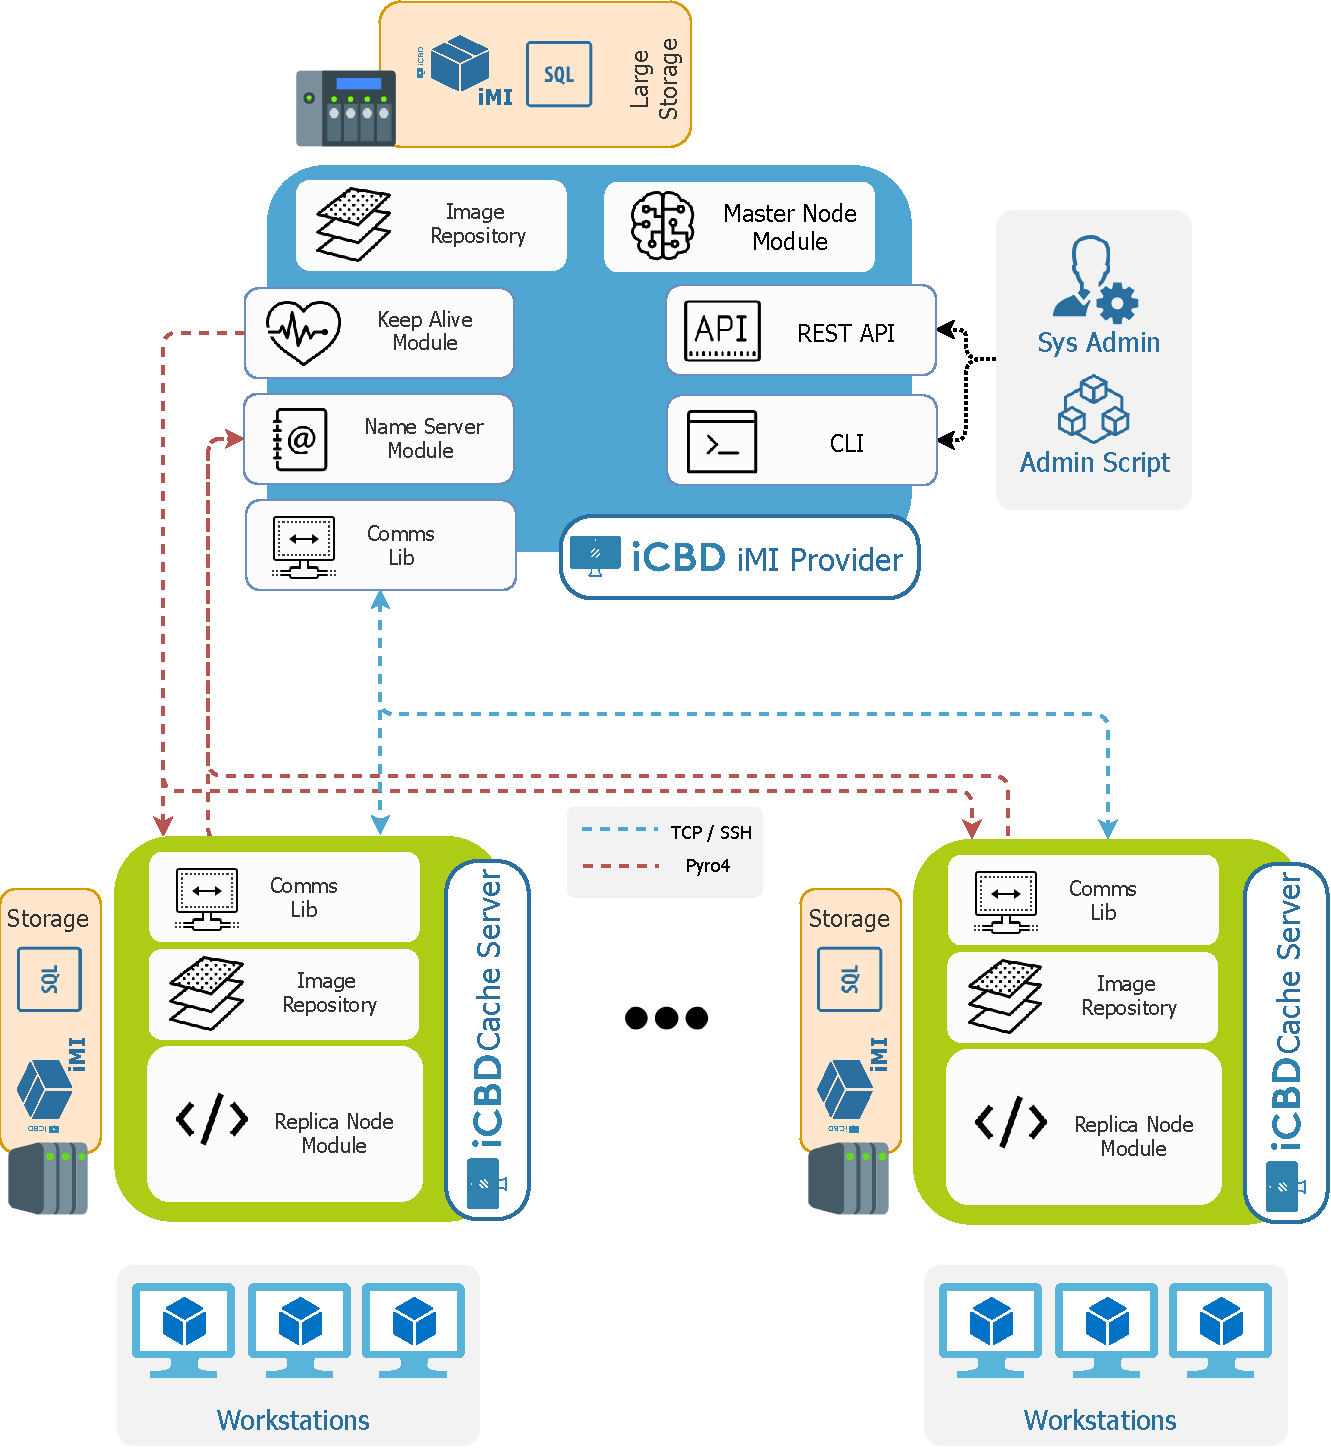
\includegraphics[height=4in, width=\textwidth]{cap4_icbd_arquit}
	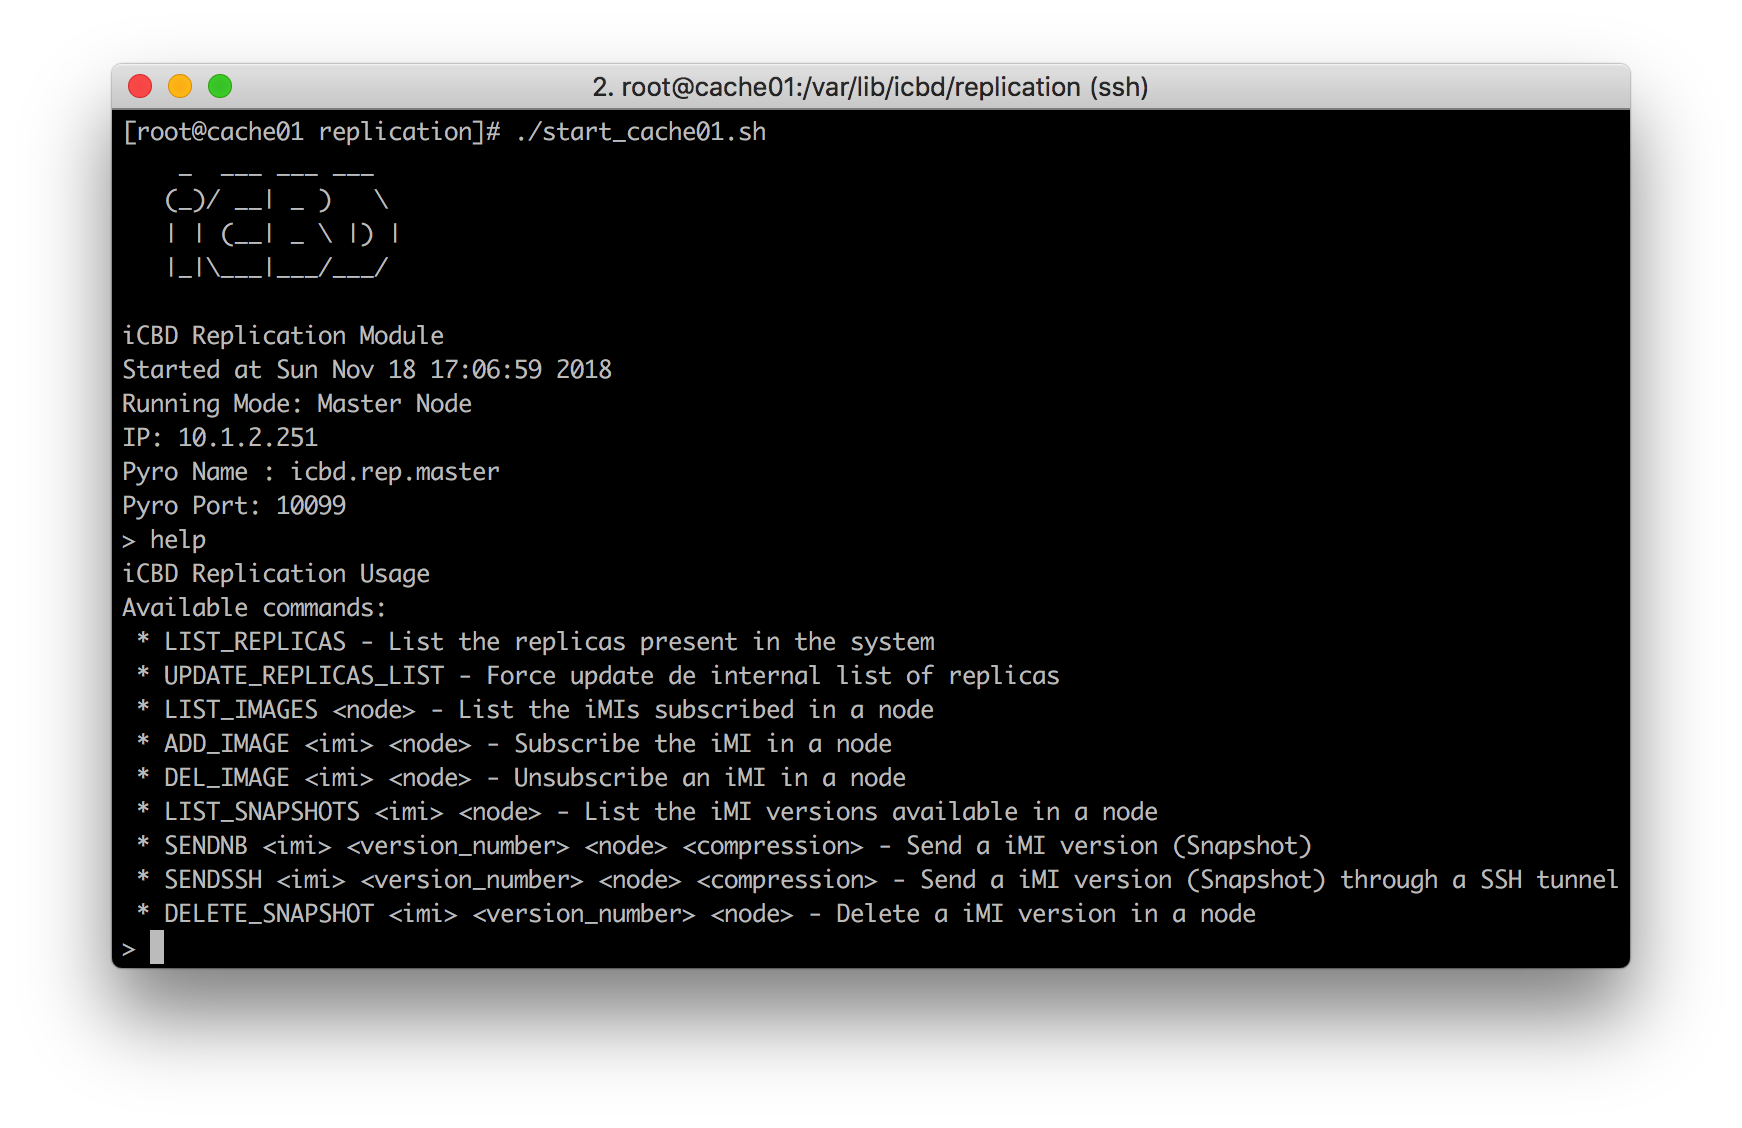
\includegraphics[width=\textwidth]{cap4_clihelp}
	\caption{iCBD Replication Module help output}
	\label{fig:icbd_rep_clihelp}
\end{figure}

%This interface, although simplistic, allows to efficiently manage all the tasks related to the replication of iMIs between the several servers of the platform. Following we demonstrate the functions provided by this interface and the effects produced on the platform:

Following we demonstrate the functions provided by this interface (the help output of the CLI is exhibited in Figure~\ref{fig:icbd_rep_clihelp}) and the effects produced on the platform:

\begin{description}
	\item \texttt{List Replicas} - At any time it is possible to consult which nodes are registered in the platform, this command allows to list the replicas registered in the Name Server and indicates which URI is used to make a connection.
	%
	\item \texttt{Force Update Name Server} - As previously explained, when a replica node stops responding, that node is deleted from the records held by the Name Server. However, this process may not be immediate because of the timeout implemented. So this feature forces an update to the Name Server list by contacting all the nodes and determining if they are working correctly.
	%
	\item \texttt{List Subscribed iMIs} - This command receives as a parameter a replica node and shows a list of which iMIs that node is interested in receiving. It should be noted that a replica node may not subscribe to an iMI but still make it available to its client (was previously subscribed and the data was not deleted), it just will not be receiving new versions as they are being produced.
	%
	\item \texttt{Subscribe iMI} - Like the previous operation, this receives some arguments (a replica node and an iMI), then, registers the interest of the replica node in a given iMI. After this procedure, this node will be able to receive versions of this iMI.
	%
	\item \texttt{Unsubscribe iMI} - When a replica node ceases to be interested in a given image present on the platform, this operation marks that new versions of the iMI should not be transferred to that node. However, all versions that have already been sent persist on the node and in order to be deleted them an appropriated operation must be used.
	%
	\item \texttt{List iMI available versions} - It is usual for a given node to contain multiple versions of an iMI (for example, the Master Node contains all versions of all iMIs that can be distributed). Thus, given an iMI, this operation allows the listing of which versions a node stores.
	%
	\item \texttt{Send iMI Snapshot} - Possibly the most significant operation in this module. It is responsible for sending the respective versions of an iMI to the intended node. Always verifying which versions are present on the target node since only the differences between versions should be sent. This command also supports the application of a compression algorithm from those provided by the platform, since it may be the case of transferring a version for the first time with a very significant data volume, or the changes between versions possess a high compression rate thus making the compression of these data advantageous.
	%
	\item \texttt{Send iMI Snapshot Secure Connection (SSH)} - This functionality is similar to the one presented above. In particular case, they share a large portion of the code, because they carry out the same operations. They only differ in the method of sending the data, which in this instance are transmitted in an encrypted fashion through an SSH tunnel. This functionality is sure to add some overhead to the transfer process, but the encryption of the data is essential in situations where the nodes are in separate networks, where there is no control wheresoever to the data security.
	%
	\item \texttt{Delete iMI version} - Finally, it is necessary to provide a way to delete versions of a given IMI in a node. Either because no longer is desired to make an IMI available or for reasons of proper management the storage space on a replica node. It is important to note that because of the way different versions of iMIs are stored in the platform, deleting older versions may not result in a space release equal to the size of the full iMI, since newer versions probably will still need this data.
\end{description}


\subsubsection{REST API}
\label{subsub:impl_icbdrep_restapi}

In order to complement the Comand-Line Interface previously presented and creating a more straightforward, more ubiquitous way of interacting with the replication platform, a Rest API has been introduced. Aiming to provide the same functionalities as the CLI but trying to create the roots of a component that deals well with platform scaling and the introduction of new features or components.

In order to integrate this component with the remaining replication platform, we employ one of the most used frameworks for creating web platforms in Python, the Flask micro-framework~\cite{flask}.

\paragraph{Flask}
\label{par:impl_flask}

Started as an April's Fool's Day joke to become the second most popular web development frameworks. Flask is a Python micro web framework designed with simplicity in mind, enabling quick deployment of applications and at the same time providing the ability to scale for complex environments. Such library enables the development of web applications without having to worry with more low-level aspects like network protocols and thread management. This framework began its development in 2010 by Armin Ronacher as a wrapper of two of his libraries: Werkzeug~\cite{werkzeug} and Jinja~\cite{jinja}.

Our use of this framework has focused only on its ability to quickly provide an environment for creating a REST API and connecting it with the rest of the replication platform. 
Next, in Listing~\ref{listing:impl_restapi}, we present the endpoints through which it is possible to interact with a master node.

\begin{listing}[ht]
\begin{description}
	\item \texttt{GET /api/replicas} - list all Replicas in the system
	\item \texttt{GET /api/replicas/\{replica\}/imis} - list of the iMis present in a Replica 
	\item \texttt{GET /api/replicas/\{replica\}/imis/subscribe/\{imi\}} - Replica subscribe to iMI 
	\item \texttt{GET /api/replicas/\{replica\}/imis/unsubscribe/\{imi\}} - Replica unsubscribe to iMI 
	\item \texttt{GET /api/replicas/\{replica\}/imis/\{imi\}/versions} - list the versions of iMI present in Replica
	\item \texttt{GET /api/replicas/\{replica\}/imis/\{imi\}/versions/\{version\}/delete} - delete a version of iMI in Replica
	\item \texttt{GET /api/master/imis/} - list the iMIs present in Master
	\item \texttt{GET /api/master/imis/\{imi\}/versions} - list versions of iMIs present in Master
	\item \texttt{GET /api/master/send?imi=\{imi\}\&version=\{version\}\&replica=\{replica\}} - send version of iMI to Replica
\end{description}
\caption{iCBD-Replication REST API Route Mapping}
\label{listing:impl_restapi}
\end{listing}


%\begin{listing}[ht]
%\inputminted{python}{./Chapters/Code/cap4_restapi}
%\caption{iCBD-Replication REST API}
%\label{listing:impl_restapi}
%\end{listing}

%\textbf{TOPICS :}
%\begin{itemize}
%	\item Flask lib
%	\item Endpoints
%\end{itemize}


%%-------------------------------------------------------------------
%%	4. - Replica Node
%%-------------------------------------------------------------------
\subsection{Replica Node}
\label{sub:impl_icbdrep_replica_node}

The replica node introduces a lightweight module that is responsible for facilitating the process of transferring and updating the iMIs that are closest to the clients.
This module responds to the question of how to simplify the process of making available iMIs closer to the client. Complementing the remaining modules of the iCBD platform, here the focus is on implementing the logic of receiving snapshots, as well as providing a way to manage which iMIs are subscribed with their different versions. With these features, we have all the components to build a cache server, something that will be explained in detail in the section~\ref{sec:impl_cache_server}.

Contrasting with the Master Node, it is not possible to interact directly with a replica; all operations will always be conducted through a Master who then is in charge of communicating with the Replica, asking him to perform those actions. This fact is more than an architectural design choice, this way we meet one of the requirements that define that a cache server should be as light as possible leaving the platform management element to a centralised location not needing to know anything concerning the overall platform state. However, there are parts in common. Similarly to the Master Node one of the components present is an Image Repository, which in this case, manages locally the iMIs and respective versions.

\paragraph{Receiving a Snapshot}
\label{par:impl_receive_snap}
By far, this functionality is the reason for the existence of this module. The process of receiving a version of an iMI is complementary to the send process explained in Section~\ref{par:impl_sendsnap} even though much more straightforward. 
As explained, the \texttt{send()} operation needs some computation resources since it has to calculate all the differences between versions to transfer, and after that step create a stream of operations that when executed recreate precisely the differences between versions. 
So, on the receiving side of this stream (in this case the Replica Node), the \texttt{receive()} operation only is only required to receive the stream, decode the operations to administer to the file system and execute them.

\paragraph{}
Documentation for all this project was generated using a tool called Sphinx~\cite{py_sphinx} and can be consulted in Annex~\ref{ann:code_docs}.

%\textbf{TOPICS :}
%\begin{itemize}
%	\item Operations on the local repository
%	\item The receive operation
%\end{itemize}




%%-------------------------------------------------------------------
%%	4. - Building a iCBD Cache Server
%%-------------------------------------------------------------------
\section{Deploying an iCBD Platform with a Cache Server}
\label{sec:impl_cache_server}

%To solve some of the enunciated problems with a DaaS solution that derive from limited bandwidth, latency and jitter from the limitation of accessing the image repositories from an internet connection and provide some scalability feature with the implementation of proximity cache servers are key. These cache servers can store replicas of the iMIs created and maintained in an administration server. Moreover, since they are located in the same LAN segment as the clients is from here that they will boot.
%For accomplishing this work, the cache servers need to have hard drives. (Although it would be possible to have diskless cache servers, they would be blocked if there was an interruption in the internet access, and it is to avoid that the local drives are necessary. )

%A instalação, configuração e administração dos cache-servers far-se-á também pela instanciação a partir da imagem de uma VM especialmente preparada para o efeito e residente na cloud, no sistema de administração. Os cache-servers arrancam inicialmente pela rede a partir do servidor na cloud e carregam um Linux que vai formatar os discos, neles instalando o conteúdo da própria imagem de VM, terminando com a instalação de um boot loader que irá arrancar o sistema do cache-server após a máquina fazer reboot. Daí em diante o sistema de administração na cloud irá disponibilizar as actualizações que forem necessárias, podendo mesmo forçar a re-instalação total dos cache-servers.

%Note-se que uma vez instalado um cache-server numa LAN, dada a grande fiabilidade que pode ser ainda reforçada através das técnicas habituais em sistemas tolerantes a faltas e de elevada disponibilidade (referir a sugerida pelo Paulo), torna-se viável a utilização de servidores diskless, instanciados a partir de VMs templates configuradas e administradas na cloud e depois replicadas para o cache-server, como nas imagens dos desktops.

%Assim como o Linux dos cache-servers é instalado nos discos locais dos servidores a partir de imagens na cloud, é possível fazer o mesmo com qualquer outra imagem de Linux que se queira. Assim, o administrador de sistema de um cliente poderá configurar outras VMs com o software e os serviços de que necessitar, designar uma máquina física como alvo, e fazer com que a VM seja vertida para os discos da sua máquina física, sendo configurado um boot loader para lhe permitir arrancar com essa configuração.

%Como os clientes nestas categorias tipicamente necessitam de dezenas, centenas ou mais de postos de trabalho, na prática é impossível suportá-los directamente a partir de repositórios remotos de VMs templates. Em vez disso, iremos recorrer a “servidores de proximidade” ou “c​ache-servers”​, máquinas Linux reais ou virtuais devidamente dimensionadas e configuradas, instaladas na LAN dos clientes, idealmente uma (ou mais) por cada segmento de rede, as quais manterão réplicas das VMs templates a que cada cliente tem acesso nos repositórios remotos.
%Com estes cache-servers localmente acessíveis aumentar-se-á drasticamente a velocidade de transferência de dados e a latência e o jitter nos acessos reduzir-se-ão a valores insignificantes, podendo cada cache-server suportar dezenas (ou mais) de PCs clientes (estimamos o número em 15 a 30 por cada interface gigabit nos cache-servers, estimativa que permanece válido para PCs clientes ligados a 100 Mbps através de switches com ligação gigabit aos cache-servers).

Once the process of creating a mechanism to support the replication of iMIs has been completed, we have reached a stage where we must tackle the set of problems that may arise when supporting a large number of clients. A short list is: limited bandwidth between the central repository and distant (in terms of latency, but also bandwidth) workstations; high latencies and jitter resulting from network congestion events and/or configuration errors in the network equipment.
We believe that bringing the iMIs closer to the workstations is a way to solve all these problems at once.

When our work started, there was already an iCBD infrastructure in place at DI-FCT/NOVA; however, all iCBD support services were deployed in a single VM, with limited resources (when we took into account that the infrastructure had a lot more resources) and tests were run on a couple of VMs that were used as a (virtual) replacement for the user’s physical workstations. And the software versions were both quite old, when compared with the iCBD development infrastructure held at SolidNetworks, and missing important features that were then available at the development site.

Those limitations originated from the fact that iCBD project had no dedicated infrastructure, it was sharing the same already scarce resources with other research projects and services at DI. Fortunately, that situation changed with the acquisition of new equipment dedicated solely to this project, and that created the perfect opportunity to re-evaluate the architecture of the iCBD services and carry out a fresh installation of the whole platform.


\subsection{The iCBD infrastructure at DI-FCT NOVA}
\label{sub:impl_infrastructure}

The core of the iCBD infrastructure at DI-FCT NOVA is a two-node cluster based on HPE ProLiant DL380 Gen9 servers interconnected via an HPE Flexfabric 5700 managed switch with 10Gbps links with external storage provided by an HPE MSA 2040 SAN Storage Disk Array.
For the “remote” nodes, i.e., the replication and cache servers, the project proposal that was submitted for funding had low-end/low-cost servers in mind; in our tests, a desktop PC that was disposed from another research project was reconditioned, and we upgraded the amount of RAM and added a second hard disk.

Finally, the workstation/client testbed was provided by two student laboratories at DI (Labs. 110 and 112), each containing 15 modern PCs (CPU - Intel Core i3-7100 @ 3.90GHz; RAM - 8 GB; Gigabit Ethernet). An important feature was the i3 CPU, which supports Intel VT and is able to run hypervisors.


The detailed specifications of all these components can be found in the tables~\ref{tab:imple_hp}, ~\ref{tab:imple_msa} and ~\ref{tab:imple_cs}.


\begin{table}[htpb]
\centering
\begin{tabular}{ll}
\textit{\textbf{CPU}}             & 2x Intel Xeon E5-2670 v3 @ 2.30GHz        \\
\textit{\textbf{Memory}}          & 128 GB                                    \\
\textit{\textbf{Controller Type}} & 12Gb/s SAS                                \\
\textit{\textbf{Ethernet}}        & 2 ports at 10 Gbps plus 4 ports at 1 Gbps \\
\textit{\textbf{Hypervisor}}      & VMware ESXi, 6.5.0, 4564106              
\end{tabular}
\caption{Specifications of one HP ProLiant DL380 Gen9 host}
\label{tab:imple_hp}
\end{table}

\newpage

\begin{table}[htpb]
\centering
\begin{tabular}{ll}
\textit{\textbf{Controllers}}    & 2 MSA 2040 SAS                          \\
\textit{\textbf{Total Capacity}} & 7.2 TB                                  \\
\textit{\textbf{Disks}}          & 12 HP SAS 600GB 10k Rpms                \\
\textit{\textbf{Host interface}} & 8 12Gb/sec SAS ports (4 per controller) \\
\textit{\textbf{Ethernet}}       & 2 ports at 1 Gbps (1 per controller)   
\end{tabular}
\caption{Specifications of the HPE MSA 2040 SAN Storage}
\label{tab:imple_msa}
\end{table}


\paragraph{iCBD Networking}
\label{par:impl_infra_network}

iCBD must be able to coexist with other services and be integrated into existing networks; therefore, we studied all types of traffic generated by the platform in order to be able to segregate it into different logical (or physical, if the need arises) networks thus preventing it from “interfering” with other services in the organisation.
At the topmost level we can subdivide the traffic in two groups: internal, restricted to the platform, which is generated by the different iCBD services when they communicate between them; and external, which can be further subdivided into general Internet access, intra-net traffic, between the core platform and remote servers or workstation clients in the labs – for example, for iMI transfer.

The iCBD core cluster runs the VMware vSphere suite, which provides advanced network virtualisation features. One of those is the Distributed vSwitch (DVS) which is a single virtual switch that spans all (or a subset of) nodes in the cluster and acts as a single point of administration for the creation of “port groups” that share a common set of characteristics (such as VLAN ID), and to whom VMs connect.

The iCBD infrastructure uses two DVSs:

\begin{description}
	%
	\item [\textit{DI DVS}] - This virtual switch, dedicated to external traffic, holds five port groups: two of them handling traffic to the two student labs, and the rest supporting the (logical) networks used by various services of the department with differentiating levels of access (students, teachers, public).
	%
	\item [\textit{iCBD DVS}] - This virtual switch, dedicated to internal cluster traffic, has port groups that differentiate the various types of traffic: management; administration of iMIs; monitoring (of traffic generated in platform tests); and, finally, traffic for the Replication and Caching System.
	%
\end{description}

Table~\ref{tab:impl_dvs} lists the relationship between the VDS portgroups and the FCT/NOVA VLANs (which are managed by an external entity – the Divisão de Infraestruturas Informáticas).

\begin{table}[]
\centering
\begin{tabular}{ll|ll}
\multicolumn{2}{c|}{\textbf{DI Distributed VSwitch}} & \multicolumn{2}{c}{\textbf{iCBD Distributed VSwitch}} \\ \hline
\multicolumn{1}{c}{\textit{Port Group}} & \multicolumn{1}{c|}{\textit{VLAN}} & \multicolumn{1}{c}{\textit{Port Group}} & \multicolumn{1}{c}{\textit{VLAN}} \\
DMZ-PRIV-DI & DMZ-PRIV-DI & iCBD-Adm-Net & VMWARE\_VMOTION\_DI \\
DMZ-PUB-DI & DMZ-PUB-DI & iCBD-Ceph & VMWARE\_VMOTION\_DI \\
LAB-DI-110 & LAB-DI-110 & iCBD-Net & VMWARE\_VMOTION\_DI \\
LAB-DI-112 & LAB-DI-112 & iCBD-Rep & VMWARE\_FT\_DI \\
R-ENSINO-PRIV-DI & R-ENSINO-PRIV-DI &  & 
\end{tabular}
\caption{Specifications of all Networks}
\label{tab:impl_dvs}
\end{table}


%%-------------------------------------------------------------------
%%	4. - Roles in the Platform
%%-------------------------------------------------------------------
\subsection{Roles in the Platform}
\label{sub:impl_roles}

%\paragraph{Roles in the Platform}
%\label{par:impl_roles}

As previously reported, from the beginning of the project, the entire platform was supported by a single VM that centralised all the services – and that is still the case in the SolidNetworks site. But, taking advantage of the new hardware, we set out to distribute the different platform services to distinct servers (physical and virtual), using the notion of roles. The current version has the following roles/servers:

\begin{description}
	%
	\item [\textit{iCBD-imgs}] This server can be considered the core of the iCBD platform, as it fulfils three iMI roles: administration (it handles the iMI administration process), storage of iMIs (in the platform storage backends), and the deployment of iMIs (to workstations). With the creation of the replication system, one more service was added to this server, since it is here that the Master Node, which manages the replication of iMIs, will run.

	For the deployment of the iCBD-imgs role, a VM with 4 vCPUs, 32GB vRAM and 2 Hard Disks (OS and Data) was created in the iCBD cluster.
	%
	\item [\textit{iCBD-rw}] This server’s key role is to make temporary read/write space available to clients, during the boot process; clients see (mount) it as a directory and, while they are running, changes that both users and system apply are saved, but only for the duration of the session; once the session is over, that data is deleted.

	One of the reasons for separating this functionality from those provided by the iCBD-imgs machine was to offer a simple way to visualise the load that results from multiple clients booting iMIs at the same time, separating that usage from reads and writes that occur during “normal” operation. Since the server’s only task is the provision of iSCSI and NFS servers that offer r/w space, we think that we can lower the RAM usage when compared with iCBD-imgs and deploy a VM with 4 vCPUs, 8GB vRAM and 2 Hard Disks (OS and Data). 
	
	As the functionality of this machine is only the provision of iSCSI and NFS servers for accessing r/w space its specifications may be a bit more conservative with a VM boasting 4 vCPUs, 8GB vRAM and 2 Hard Disks (OS and Data).
	%
	\item [\textit{iCBD-home}] This is an optional role, for an NFS-based service that handles access to user home directories, which makes sense in an environment where a large community uses Linux. The iCBD-home server will either host the storage itself or consume it from a storage backend; in any case it will hold the user’s home directories and export them to the user’s workstations in a secure way, in a straightforward process: each user has a home directory under the iCBD-home server’s \texttt{/home}; then, when the user boots his/her workstation from a Linux iMI, that directory is exported by NFS and mounted in the workstation’s \texttt{/home}, thus enabling the user to log in and access its contents.
	The iCBD-home could also, in theory, act, in a Windows environment, as a gateway to a CIFS server; however, support for this type of “remote storage” for Windows clients was not implemented in our project.

	The specifications for the iCBD-home VM are very similar to those of iCBD-rw, with the exception of the size of the second, “data”, disk - which could be zero, if that storage was provided by an external storage server, to the amount deemed suitable for the particular iCBD installation.
	%
	\begin{table}[]
\centering
\begin{tabular}{lccccc}
 & \textbf{vCPU} & \textbf{vRam} & \textbf{Hard Disks} & \textbf{Interfaces} & \textbf{OS} \\ \cline{2-6} 
\textit{iCBD-imgs} & 4 & 32 GB & 16 GB + 600 GB & 5 & CentOS 7 \\
\textit{iCBD-rw} & 4 & 8 GB & 16 GB + 300 GB & 4 & CentOS 7 \\
\textit{iCBD-home} & 4 & 8 GB & 16 GB + 100 GB & 4 & CentOS 7 \\
\textit{iCBD-cache} & 4 & 32 GB & 16 GB + 600 GB & 2 & CentOS 7 \\
\textit{iCBD-client} & 4 & 8 GB & Diskless & 1 & Network Boot
\end{tabular}
\caption{Specifications of the virtual hardware of the iCBD machines}
\label{tab:impl_VM_Specs}
\end{table}

	\item [\textit{iCBD-cache}] This was the service (a.k.a. Cache Server) that we have architected, designed, implemented and deployed in this thesis. From the client’s point-of-view, it is indistinguishable from the iCBD-imgs service that provisions iMIs to workstations but, with the introduction of RCS, each Cache Server also runs the Replica Node service (introduced in Section~\ref{sub:impl_icbdrep_replica_node}), aiming to reduce the latency and increase the transmission rate between the image server and the workstations, thus improving the user’s experience. It may be implemented, as it was the case with the other roles, on physical or virtualised hardware. 

	On the DI-FCT/NOVA site, two types of cache servers were set up: a virtual machine, because it was easier to deploy and test the correctness of its operation; and, later on, a physical server that was connected directly to one of the students’ labs and was responsible for delivering the iMIs to that lab’s workstations. Both configurations can be seen in the tables~\ref{tab:impl_VM_Specs} and ~\ref{tab:imple_cs}, respectively.
	%
	\item [\textit{iCBD-admin\_iMI}] This is a special role created specifically for the administration of iMIs. The process of administering an iMI is triggered and managed by scripts that run within the iCBD-imgs server, but since administration always involves the need to run a VM based on the iMI we want to manage, this process can be carried out in two different ways: in the iCBD-imgs server itself, in nested virtualisation mode; or, running the iCBD-admin\_iMI VM as yet another VM running in the iCBD cluster.
	
	\textbf{Nested virtualisation mode}  Here the iCBD-admin\_iMI VM is executed under a VMware Workstation (or Player) Type II hypervisor, i.e., an hypervisor that executes as a OS process in a CentOS (our default choice) or another suitable hosting OS. Running in nested virtualisation mode has a moderate-to-high decrease in performance.
	 
	\textbf{Standard virtualisation mode}  Here the iCBD-admin\_iMI VM is executed directly on the VMware vSphere Type I (a.k.a. native, or bare-metal) hypervisor, i.e., an hypervisor that executes directly on the server’s hardware.
	
	Whatever our choice is, the iCBD-admin\_iMI VM is created dynamically by the administration process and works in a similar way to a client, with a difference: changes made to the IMI may be committed and used to create a new version of that iMI.
	%
	\item [\textit{iCBD-client}] The platform client is the simplest of roles. Again, there are two cases, depending on whether the client is a physical workstation or a VM: we can create a diskless virtual machine, and connect it to a network where an image server (iCBD-imgs or iCBD-cache) is located (visible) and boot the VM using a network boot process – the result is an iMI being provided to that to that VM, the TFTP will transfer the kernel,…, (as was largely described in section~\ref{subsub:icbd_booting_imi}) and the client will end running the chosen OS. Naturally, the same process can be used for a workstation provided that the physical network has connectivity to the appropriate iCBD networks. Furthermore, other ways to boot an iMI on a workstation, such as creating a bootable USB drive that connects the workstation to an image server, without using DHCP or PXE, are possible.
	%
\end{description}

\begin{table}[htpb]
\centering
\begin{tabular}{ll}
\textit{\textbf{CPU}} 		& Intel Core i5-650 @ 3.20GHz \\
\textit{\textbf{Memory}} 	& 12 GB \\
\textit{\textbf{Storage}} 	& 2x SATA 80 GB  + SATA 160 GB \\
\textit{\textbf{Ethernet}} 	& 2 ports at 1 Gbps \\
\textit{\textbf{OS}} 		& CentOS 7 3.10.0-514
\end{tabular}
\caption{Specifications of the Physical Cache Server}
\label{tab:imple_cs}
\end{table}



\subsection{Installing iCBD Core Services}
%\paragraph{Installing iCBD Core Services}
\label{sub:impl_install_icbd_core}
%Found a Centos 7 kernel bug.
%https://bugs.centos.org/view.php?id=14228
%https://bugzilla.redhat.com/show_bug.cgi

As one may deduce from the number of roles described above and the complexity of their interactions, deploying the iCBD platform (services), even with the enormous benefits brought by virtualisation, is not a trivial task.
First, the networking infrastructure connections must be made, and then the configuration must be deployed. Deploying the network configuration is a slow process because it involves many interactions with the Faculty group that is responsible for networking infrastructures at the university campus. The VLANs, security/firewall policies, etc., all must be defined and “negotiated”, as the iCBD switches must be managed by that same group (that is understandable because if they were managed by any other group – ourselves included – the opportunity for “breaking the rules” / “violating the policies” would be there).  New policies had to be defined so that the iCBD servers could “tap” into the student’s labs, for PXE booting, TFTP and/or HTTP image transfer,  and NFS or iSCSI mounting all were transparently handled without jeopardising the labs normal operation.

The installation process was carried out in three phases. In the first phase, VMs for the various services (roles) - iCBD-imgs, iCBD-rw, and iCBD-home – were created from a vSphere template with a minimal CentOS 7 installation. Then, for each VM, the CentOS packages and other software that was necessary to support the role were installed and configured. Finally, some iMIs that were already available in the SolidNetworks site were transferred and prepared to operate in the DI site. At the end of the first phase, VMs posing as workstations could be started inside the cluster and boot the available iMIs.

The creation of multiple virtualised Cache Servers constitutes the second phase. The creation of these VMs was an easy step because the iCBD-imgs was used as a base VM from which the first Cache Server VM was created, through the use of a full cloning procedure. Then, the unnecessary functionalities (with regard to the new role) were removed, and the modules that provide the Replication service were added. This step was crucial to create a test environment for the replication modules, which before this phase, had not been tested with production iMIs.

The last phase was the installation of a single physical Cache Server as close as possible to one of the labs, and that was accomplished by plugging it directly to the switch that interconnected all the lab 
workstations. So, we successfully reached a point where we had two setups with access to the iCBD platform: one, where the lab’s 15 PCs were able to get their IMIs from a (physical) Cache Server; the other, where the lab’s 15 PCs had to get their iMIs from the iCBD-imgs virtual machine hosted in the cluster.

The process of creating a single VM for the iCBD platform is, obviously, quite cumbersome (despite the short description we gave when discussing the first phase) and with some significant details that must be addressed. So, we have provided in Annex~\ref{ann:icdb_install} a document that was produced when the installation process of the iCBD DI platform was carried out. The document provides, we believe, a detailed and clear explanation of all steps needed to create the VM, and then install and configure each iCBD service.

\paragraph{Btrfs bug found in CentOS 7 Kernel}
\label{par:impl_centos_bug}

As a curiosity, during the process of building the iCBD-imgs VM, we found a bug in a fundamental component of the \textit{coreutils} tool delivered with the CentOS 7 kernel version \texttt{3.10.0-693.5.2}: the \texttt{cp} command, when used with option \texttt{--reflink=always}, failed with the error message ``failed to clone `someFile': Operation not supported''. This behaviour was reported to both CentOS and Red Hat and was eventually fixed. A more in-depth description of this process can be found in Annex~\ref{ann:bug}.







%!TEX root = ../template.tex
%%%%%%%%%%%%%%%%%%%%%%%%%%%%%%%%%%%%%%%%%%%%%%%%%%%%%%%%%%%%%%%%%%%%
%% chapter5.tex
%% NOVA thesis document file
%%
%% Chapter with lots of dummy text
%%%%%%%%%%%%%%%%%%%%%%%%%%%%%%%%%%%%%%%%%%%%%%%%%%%%%%%%%%%%%%%%%%%%
\chapter{Evaluation}
\label{cha:evaluation}

%\textbf{TOPICS :}
%\begin{itemize}
%	\item Benchmark the iCBD-Replication Module
%	\item Assert the performance gained by storing iMI closer to client workstations
%\end{itemize}

The following chapter reports the experimental work performed in order to study both the executability and performance of the Replication and Caching Service. We describe the tests defined and performed following with some analysis of the results obtained, always trying to co-relate to the effects observed throughout the platform.

The chapter is divided into the following sections:

\begin{description}
    %
    \item [Section~\ref{sec:eval_exp_setup}] .
    %
    \item [Section~\ref{sec:eval_method}] ..
    %
    \item [Section~\ref{sec:eval_rep_bench}] ..
    %
    \item [Section~\ref{sub:eval_cache_bench}] ..
    %
\end{description}

%%-------------------------------------------------------------------
%%	5. - Motivation
%%-------------------------------------------------------------------
%\section{Motivation}
%\label{sec:eval_motivation}

%https://stackoverflow.com/questions/1198691/testing-io-performance-in-linux
%https://dl.acm.org/citation.cfm?id=1367829.1367831

%https://github.com/axboe/fio
%https://github.com/giantswarm/filesystem-benchmark


%%-------------------------------------------------------------------
%%	5. - Experimental Setup
%%-------------------------------------------------------------------
\section{Experimental Setup}
\label{sec:eval_exp_setup}

To ensure the correct execution of all the tests we intended to carry out some adjustments to the iCBD platforms were necessary. To the infrastructure, we deployed two more virtual cache servers (adding to the physical cache server already in operation) with the entire iCBD solution including the RCS. 

Also as discussed in the previous chapter, the Computer Science Department provided two laboratories (Lab 110 and Lab. 112) fully equipped with fifteen machines each (the general specifications of these machines can be seen in the table~\ref{tab:exp_lab_work}), with the objective of performing validation testing of the caching solution at a functional level and then the execution of performance tests.

\begin{table}[]
\centering
\begin{tabular}{ll}
\textbf{CPU} & Intel Core i3-7100 @ 3.90GHz \\
\textbf{Memory} & 8 GB \\
\textbf{Storage} & 275GB SSD \\
\textbf{Ethernet} & 1 Gbps
\end{tabular}
\caption{Specifications of the Laboratories Workstations}
\label{tab:exp_lab_work}
\end{table}

There was also a need to make some changes to VMs that were already deployed, in order to make the laboratories fully functional. First, the VMs iCBD-rw and iCBD-home were connected to the networks of both laboratories configuring the interfaces with fixed IPs. Then, one interface of the iCBD-imgs VM was set up to be connected to the Lab. 110 network and also assigned a fixed IP, then some changes were performed in the iCBD configuration files to allow workstations connected to this network access to iMIs. Also, in the Physical Cache Server, one of the interfaces was configured in the network of Lab. 112, and similar configurations were necessary for this server to provide iMIs to the workstations of this Laboratory.

It is still important to note two aspects, first the Physical Cache Server and the Lab. 112 workstations are attached to the same managed switch, so the communications between them only cross this device. Whereas all communications between workstations of both laboratories and VMs deploy in the cluster travel through various equipment in the FCT NOVA network and therefore may suffer from adverse network conditions entirely out of our control. Second, all of these connections described above are ensured by Gigabit links, either at the level of the network equipment or by the interfaces (virtual or physical) of the servers. A simplistic schematic of all these connections can be found in Figure~\ref{fig:eval_setup}.

\begin{figure}[htbp]
	\centering
	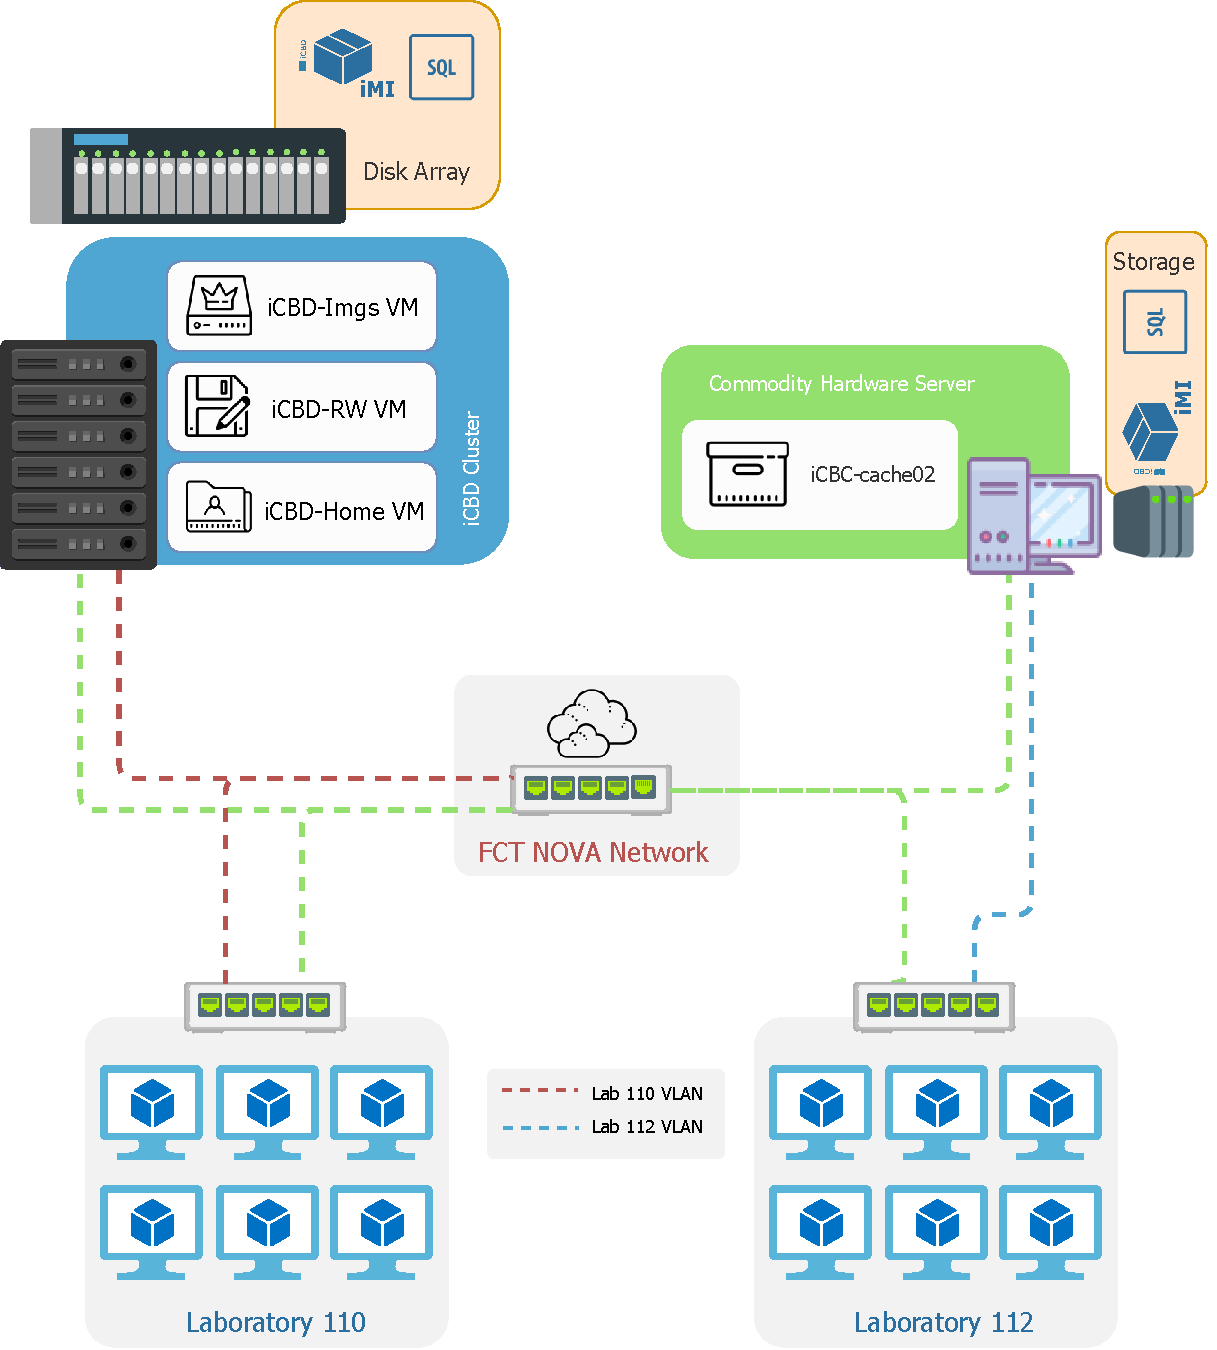
\includegraphics[height=4in]{cap5_lab_setup}
	\caption{iCBD Nodes and Networking Setup}
	\label{fig:eval_setup}
\end{figure}

\begin{table}[htpb]
\centering
\begin{tabular}{lcc}
%\hline
                             & \textbf{FCT NOVA}          & \textbf{SolidNetworks (Development)}              \\ \hline
\textit{\textbf{Servers}}    & 2x HPE ProLiant DL380 Gen9 & 2 x HPE ProLiant DL380 Gen9   \\
\textit{\textbf{Switch}}     & HPE Flexfabric 5700 jg898a & HPE Flexfabric 5700 jg898a    \\
\textit{\textbf{Disk Array}} & HPE MSA 2040 SAN Storage   & N/A - (Storage on the Server) \\
\textit{\textbf{Networking}} & 10 Gbps (between servers)  & 10 Gbps (between servers)     \\ \hline
\end{tabular}
\caption{Physical infrastructure of the FCT NOVA and SolidNetworks sites}
\end{table}


%%-------------------------------------------------------------------
%%	5. - Metodology
%%-------------------------------------------------------------------
\section{Metodology}
\label{sec:eval_method}

The analysis of the RCS was divided into two distinct moments: a first part, which addressed the functional validation of both components of the RCS after being integrated into the iCBD platform, testing its execution correction; and a second part in which we focused on the performance of these components when faced with a production environment.

\paragraph{Functional validation}
\label{par:eval_func_val}

Concerning the replication module, in order to test that this system is functional in a multi-node environment, the Master Node was started in the iCBD-imgs VM and three Replica Nodes, one in each Cache servers (virtual - iCBD-cache01 \& iCBD-Cache03 and physical - iCBD-Cache02). Being observed that the Replica Node had registered on the Name Server as expected and that the communications between the Master Node and Replicas were done correctly.

Next, were carried out two types of test repeatedly. One focused on sending a complete version of an IMI that was not present in the Replicas' Image Repository, forcing the transportation of all the data that are part of this iMIs. We also took advantage of this moment to verify if after the sending process the local Image Repository reflected the addition of the new iMI. This scenario is likely to occur when its the first time that a replica subscribes to a new iMI.

The second type of test revolved about sending versions of iMIs that Replicas already possessed older ones in their repository. This is done to simulate the case where after the administration of an iMI this update is distributed by the Replicas with only the changed data being sent. At the end of each of these tests, we performed a calculation of an MD5 hash with the \texttt{md5sum} tool, in order to ensure that the received data was being reliably transferred.

In order to validate the correct functioning of Cache Servers we mainly focused on iCBD-cache02 (Physical Cache Server), mostly because it was connected directly to one of the laboratories allowing for immediate testing of a workstation iMI boot. Given the integration of the iCBD platform with the remaining network services and policies of  FCT NOVA, a considerable iterative process of experimentation was required, constantly tuning some parameters of some iCBD services until we arrived at a fully functional configuration.
In the end, it was confirmed that it is possible to boot the workstations with iMIs powered by the Cache Server.

\paragraph{Performance Benchmarking}
\label{par:eval_perf_bench}

In this second phase of testing, the goal was to ascertain the performance of RCS in a production environment. In the case of the replication module, we make a comparison between multiple configurations of our solution (with or without compression and secure communications) and the \texttt{rsync} tool, measuring both the time spent on the transference process as well the amount of data transmitted between nodes.

While in the performance tests concerning the cache server, we measured the time spent on the boot process of a workstation. Comparing when the iMI was provided by the Cache Server or by the iCBD-imgs VM hosted at the cluster with more significant resources. For these test batteries, we consider the boot time the time elapsed from the beginning of a load of a kernel until the initialisation of all the services in userspace is finished, making use of the tool \texttt{systemd-analyze}.

Unless stated otherwise, all tests were executed five times removing the best and worst result. The final result is the average of the remaining values. The results of the work performed in these two fields are demonstrated in the following sections.

\newpage



%%-------------------------------------------------------------------
%%	5. - Replication Service Benchmark
%%-------------------------------------------------------------------
\section{Replication Service Benchmark}
\label{sec:eval_rep_bench}

\subsubsection{Sending a complete version of an iMI}
\label{susub:eval_iMI_full}

\subsubsection{Sending only the delta between version of an iMI}
\label{susub:eval_iMI_delta}

%\textbf{TOPICS :}
%\begin{itemize}
%	\item Replication with rsync (100 / 1000 mbps)
%	\item Replication with iCBD-Replication - Plain Sockets and No Compression (100 / 1000 mbps)
%	\item Replication with iCBD-Replication - Plain Sockets and LZ4 Compression (100 / 1000 mbps)
%	\item Replication with iCBD-Replication - Plain Sockets and zlib Compression (100 / 1000 mbps)
%	\item Replication with iCBD-Replication - Plain Sockets and snappy Compression (100 / 1000 mbps)
%	\item Replication with iCBD-Replication - SSH and No Compression (100 / 1000 mbps)
%\end{itemize}

%https://stackoverflow.com/questions/5357601/whats-the-difference-between-unit-tests-and-integration-tests

% Unit Test Python
%https://docs.python.org/2/library/unittest.html

%Memory profile of the module
%https://pypi.python.org/pypi/memory_profiler




%%-------------------------------------------------------------------
%%	5. - Cache Server Performance Benchmark
%%-------------------------------------------------------------------
\section{Cache Server Performance Benchmark}
\label{sub:eval_cache_bench}

\begin{figure}[htbp]
	\centering
	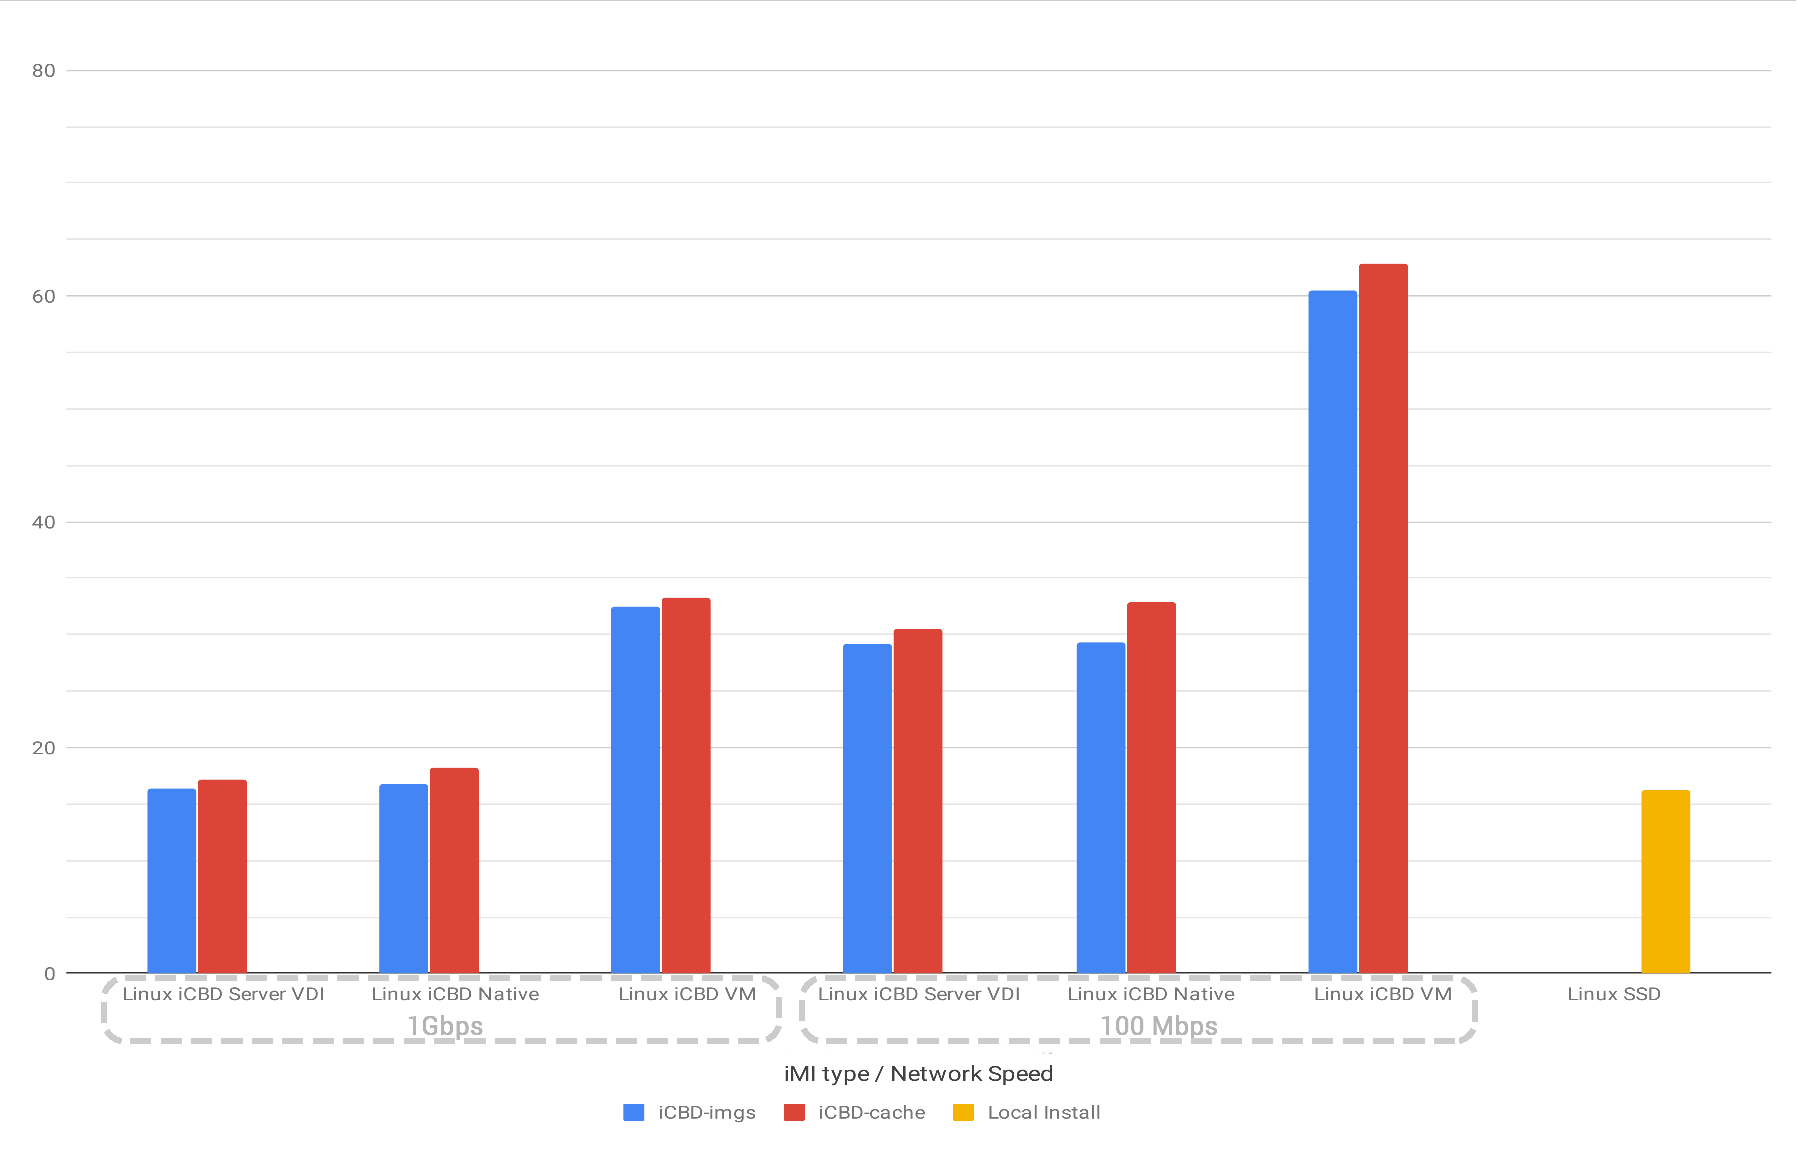
\includegraphics[height=4in]{cap5_NB_iSCSI}
	\caption{Mean Boot Time of five workstations using iSCSI (Sequential Boot Scenario), comparing iMI provider and network speed}
	\label{fig:boot_iscsi}
\end{figure}

\begin{figure}[htbp]
	\centering
	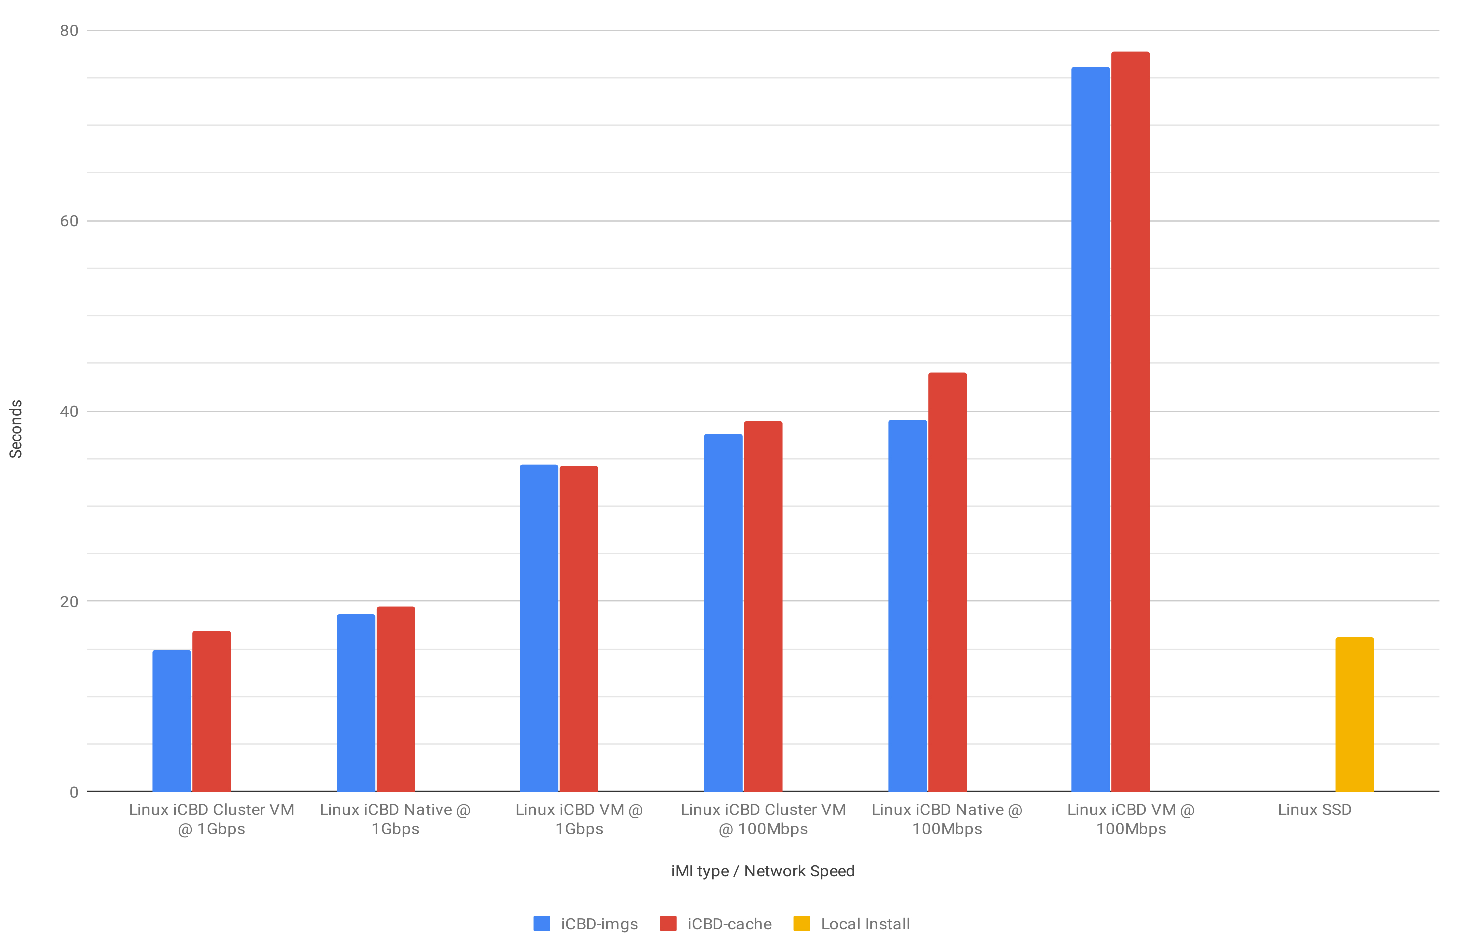
\includegraphics[height=4in]{cap5_NB_NFS}
	\caption{Mean Boot Time of five workstations using NFS (Sequential Boot Scenario), comparing iMI provider and network speed}
	\label{fig:boot_nfs}
\end{figure}

\begin{table}[]
\centering
\begin{tabular}{llcc}
\textbf{iMI} &  & \textbf{iCBD-imgs} & \textbf{iCBD-Cache02} \\ \hline
\multirow{2}{*}{\textit{Ubuntu 14.04 - Client Cluster}} & iSCSI & 453.5 MB & 454.3 MB \\
 & NFS & 703.0 MB & 702.1 MB \\ \hline
\multirow{2}{*}{\textit{Ubuntu 14.04 - Client Native}} & iSCSI & 456.3 MB & 453.6 MB \\
 & NFS & 704.2 MB & 703.8 MB \\ \hline
\multirow{2}{*}{\textit{Ubuntu 14.04 - Client VM}} & iSCSI & 834.1 MB & 836.8 MB \\
 & NFS & 950.5 MB & 952.8 MB
\end{tabular}
\caption{Total data received after booting, given each boot variant and for both iMI providers}
\label{tab:boot_totaldata}
\end{table}

\subsubsection{Benchmark in a Boot Storm condition}
\label{susub:eval_cache_bootstorm}

\begin{table}[]
\centering
\begin{tabular}{llcc}
\textbf{iMI} & \textbf{} & \textbf{iCBD-imgs} & \textbf{iCBD-Cache02} \\ \hline
\multirow{2}{*}{\textit{Linux iCBD Client Native}} & iSCSI & 20.035 s & 23.020 s \\
 & NFS & 23.248 s & 28.156 s \\ \hline
\multirow{2}{*}{\textit{Linux iCBD Client VM}} & iSCSI & 42.627 s & 52.952 s \\
 & NFS & 44.734 s & 54.840 s
\end{tabular}
	\caption{Comparison of boot times in a boot storm situation in both providers (iCBD-imgs and iCBD-cache02)}
	\label{tab:bootstorm_both}
\end{table}


\begin{figure}[htbp]
	\centering
	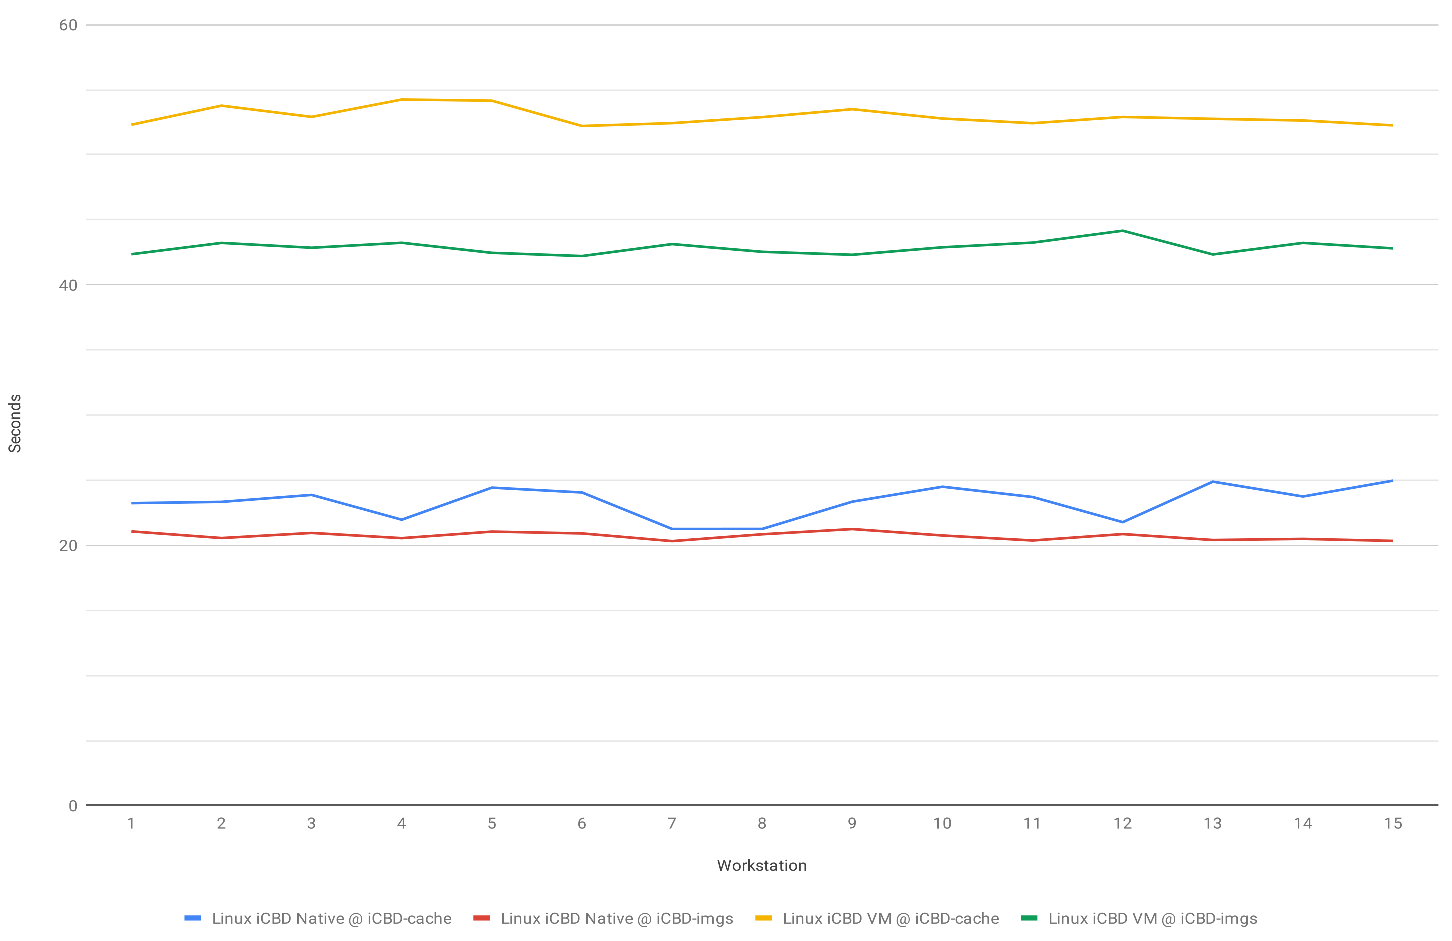
\includegraphics[height=4in]{cap5_BS_combo}
	\caption{Boot Time of fifteen workstations simultaneously (Boot Storm Scenario) comparing iMI provider}
	\label{fig:bootstorm_time}
\end{figure}


\subsubsection{iMI provider system load}
\label{susub:eval_sys_load}

\begin{figure}[htbp]
	\centering
	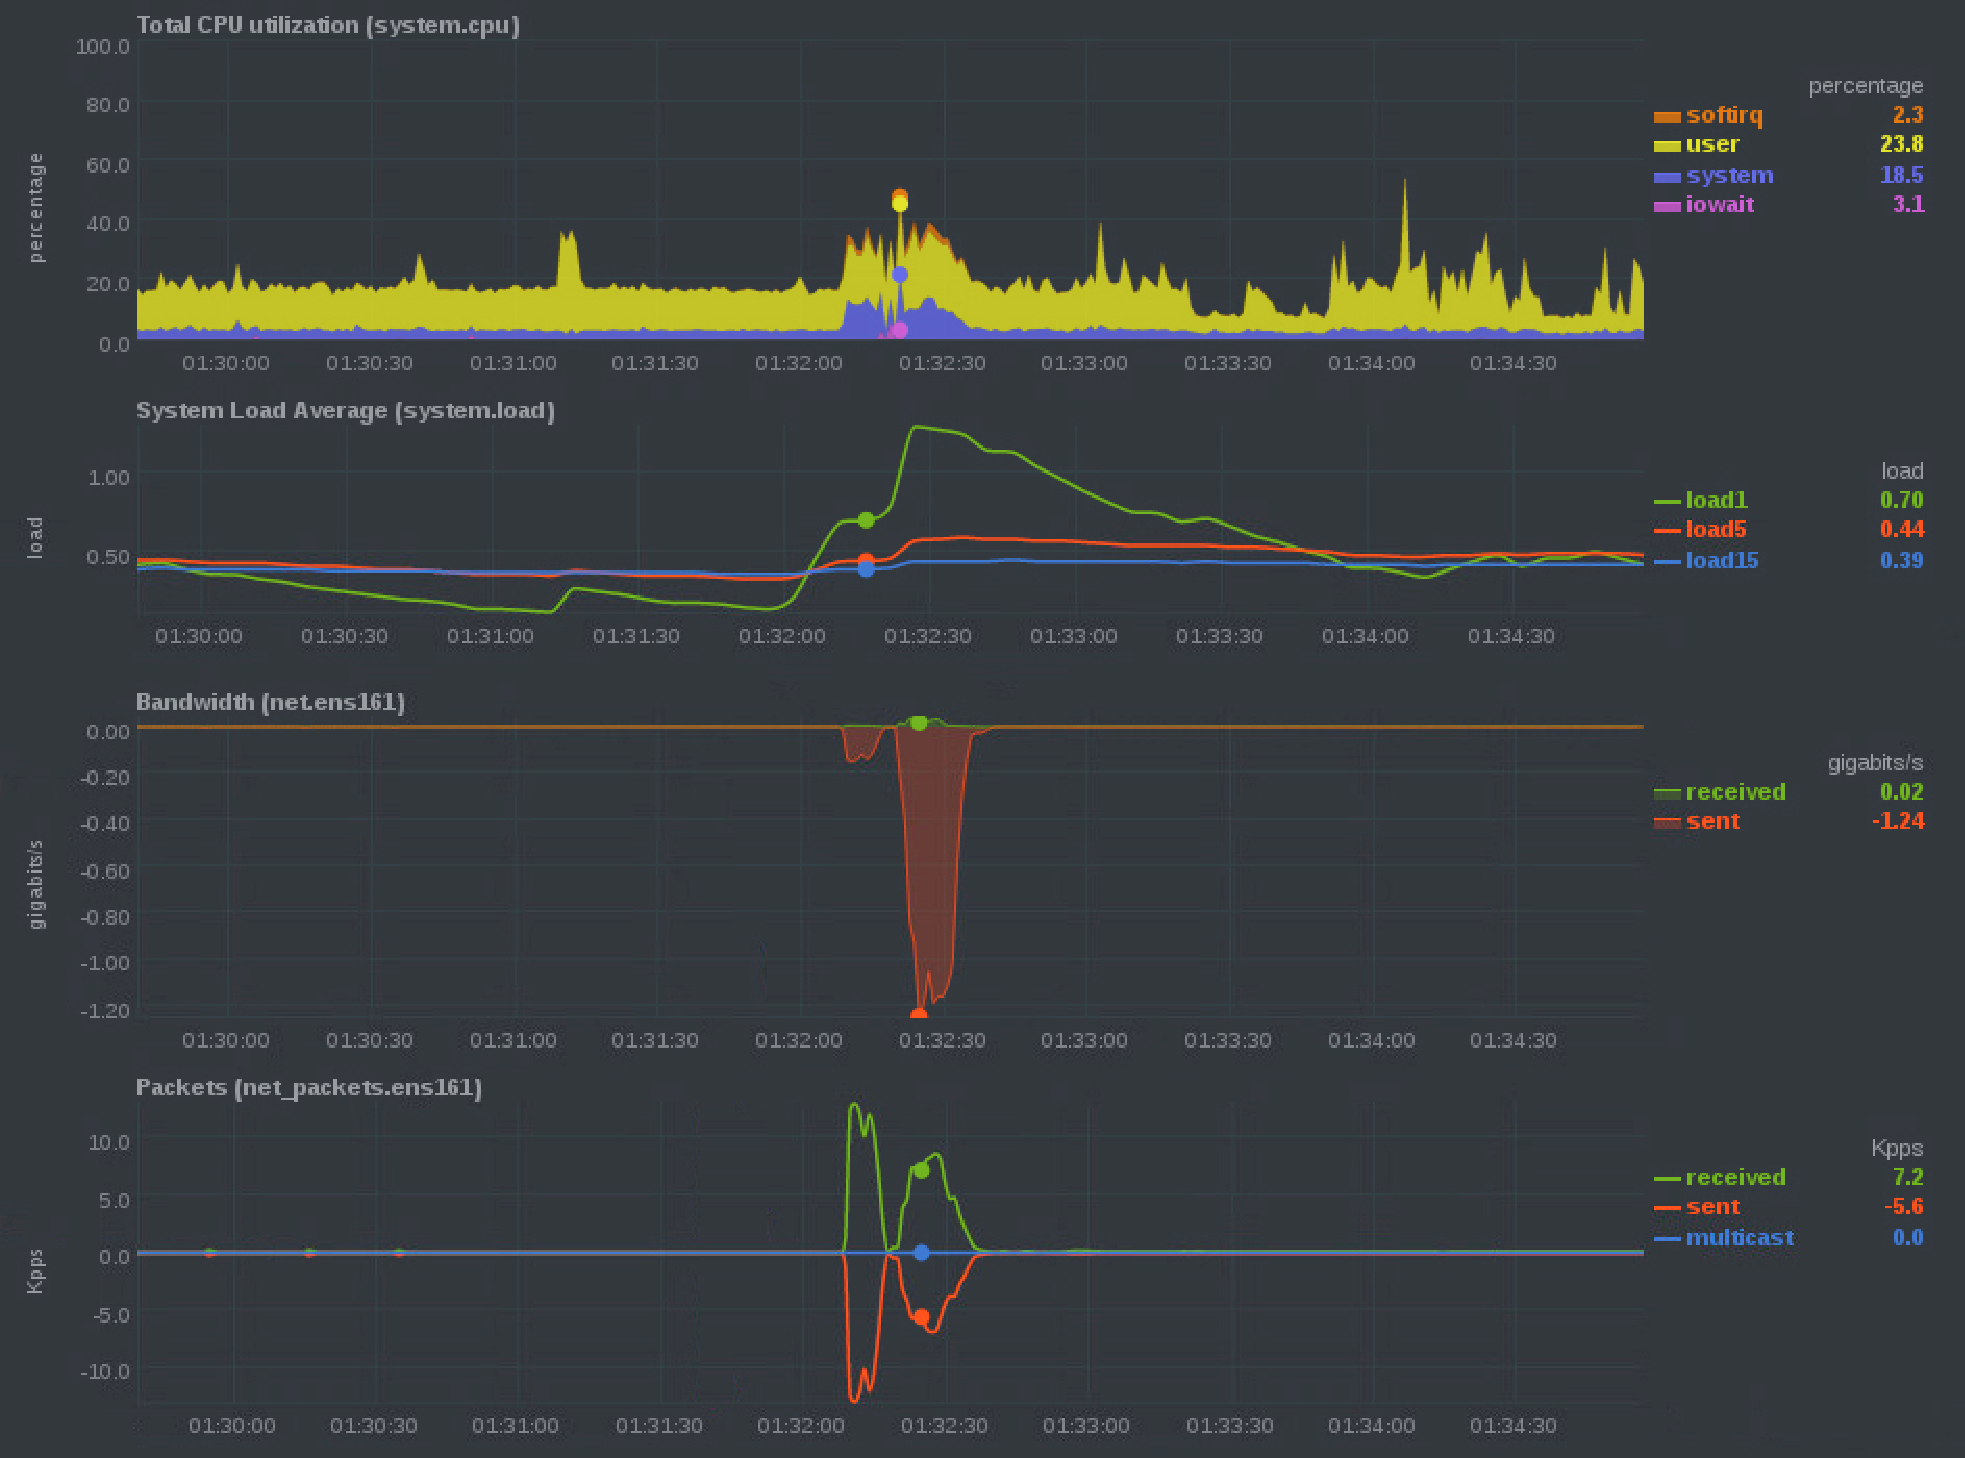
\includegraphics[height=4in]{cap5_secboot_imgs_stats}
	\caption{System metrics for iCBD-imgs on one run of the five workstations sequential boot scenario test}
	\label{fig:boot_imgs_stats}
\end{figure}


\begin{figure}[htbp]
	\centering
	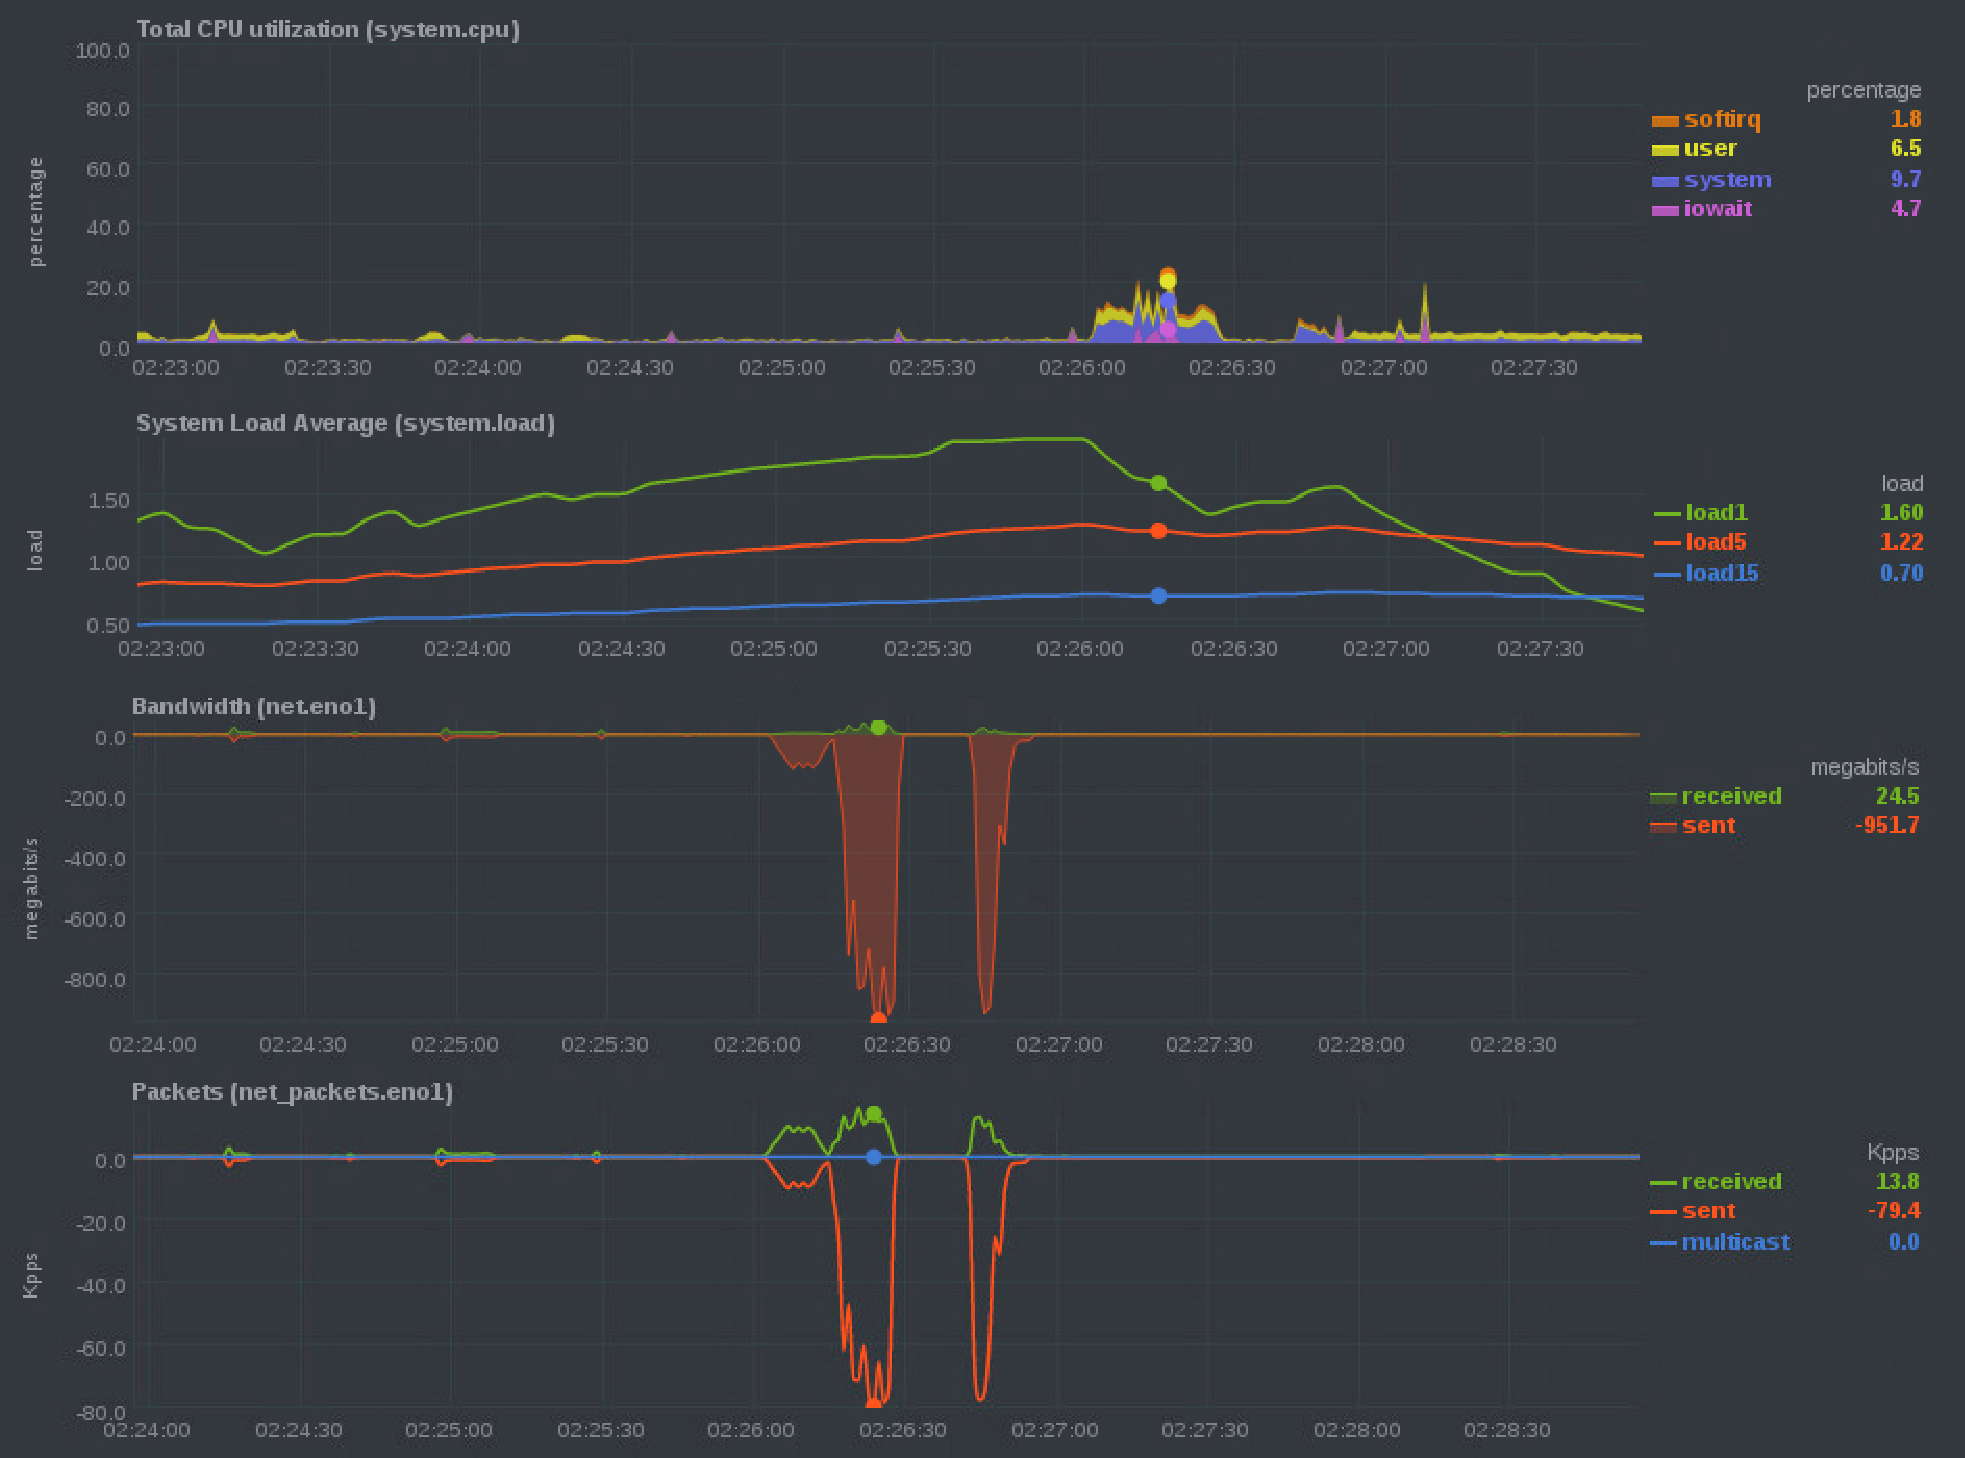
\includegraphics[height=4in]{cap5_secboot_cache_stats}
	\caption{System metrics for iCBD-Cache02 on one run of the five workstations sequential boot scenario test}
	\label{fig:boot_cache_stats}
\end{figure}


\begin{figure}[htbp]
	\centering
	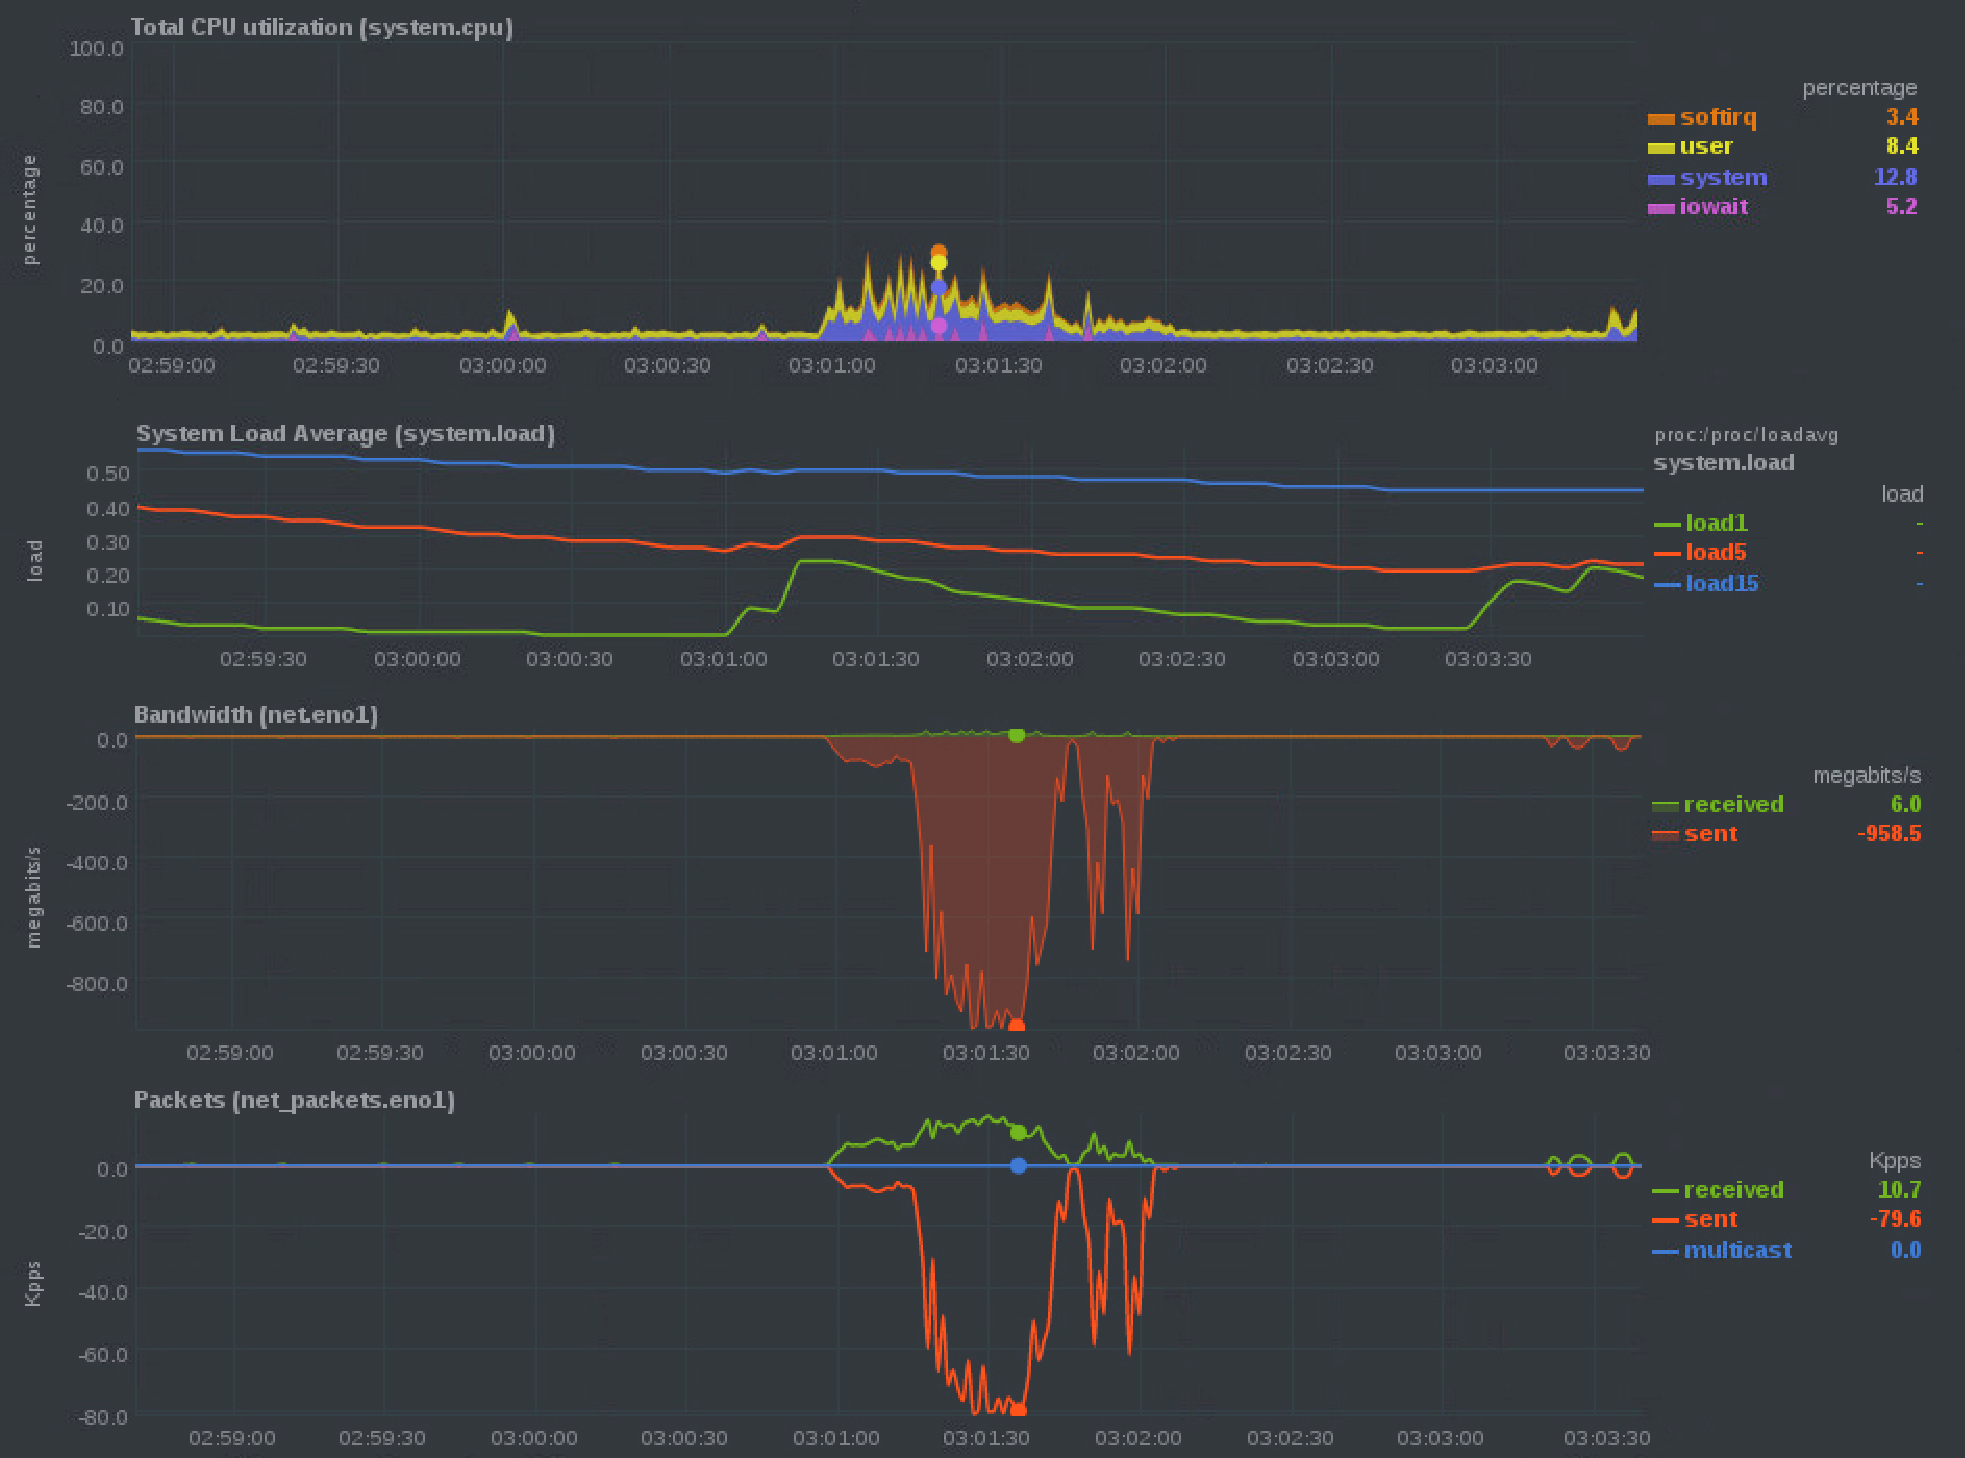
\includegraphics[height=4in]{cap5_bootstorm_cache_stats}
	\caption{System metrics for one run on the iCBD-Cache02 in a boot storm scenario}
	\label{fig:boot_cache_stats}
\end{figure}


%\textbf{TOPICS :}
%\begin{itemize}
%	\item benchmarking 
%	\item Boot time Lab PC
%	\item Boot time iCBD VM in Cluster
%	\item Boot time iCBD in Lab PC (100 / 1000 mbps) iCBD-Imgs VM
%	\item Boot time iCBD in Lab PC (100 / 1000 mbps) iCBD-Cache
%\end{itemize}
%!TEX root = ../template.tex
%%%%%%%%%%%%%%%%%%%%%%%%%%%%%%%%%%%%%%%%%%%%%%%%%%%%%%%%%%%%%%%%%%%%
%% chapter6.tex
%% NOVA thesis document file
%%
%% Chapter with lots of dummy text
%%%%%%%%%%%%%%%%%%%%%%%%%%%%%%%%%%%%%%%%%%%%%%%%%%%%%%%%%%%%%%%%%%%%
\chapter{Conclusions \& Future Work}
\label{cha:conclusion}

\section{Conclusions}
\label{sec:conclusions}

\textbf{TOPICS :}
\begin{itemize}
	\item The requirements of the implementation of the iCBD-Replication were achieved 
	\item Simple replication of iMI though multiple nodes with a subscription model, where the node only receives the iMIs that really want.
	\item Successful creation of a complete iCBD platform in FCT NOVA campus.
	\item Two department lab running the solution as a trial, and instrumental in getting experimental results
\end{itemize}

%As a result of our research and experimentation, we found that:

%\begin{itemize}
%	\item bla..
%\end{itemize}

\section{Future Work}
\label{sec:future_work}

\textbf{TOPICS :}
\begin{itemize}
	\item Replica to Replica iMI transfer
	\item Diskless Servers / selfhosting - provision iCBD Servers from iMI
	\item Micro Services, as started with this thesis (building iCBD-Replication as a standalone application) the functionalities of the iCBD Core can be segmented in multiple small services, in order to achieve a better use of resources and an easier deployment in a multi homed scenario.
	\item Infrastructure as Code, orchestrate and automate all the process described in the chapter Implementation of a Cache Server.
\end{itemize}





%%!TEX root = ../template.tex
%%%%%%%%%%%%%%%%%%%%%%%%%%%%%%%%%%%%%%%%%%%%%%%%%%%%%%%%%%%%%%%%%%%%
%% chapter7.tex
%% NOVA thesis document file
%%
%% Chapter with lots of dummy text
%%%%%%%%%%%%%%%%%%%%%%%%%%%%%%%%%%%%%%%%%%%%%%%%%%%%%%%%%%%%%%%%%%%%
\chapter{Conclusions \& Future Work}
\label{cha:conclusion}

\section{Conclusions}
\label{sec:conclusions}

\section{Future Work}
\label{sec:future_work}
%%%%%%%%%%%%%%%%%%%%%%%%%%%%%%%%%%%%%%%%%%%%%%%%%%%%%%%%%%%%%%%%%%%%%
%% appendix1.tex
%% NOVA thesis document file
%%
%% Chapter with example of appendix with a short dummy text
%%%%%%%%%%%%%%%%%%%%%%%%%%%%%%%%%%%%%%%%%%%%%%%%%%%%%%%%%%%%%%%%%%%%
\chapter{Appendix 1 Lorem Ipsum}
\label{app:lorem_ipsum1}

\lipsum[1-5]
%%!TEX root = ../template.tex
%%%%%%%%%%%%%%%%%%%%%%%%%%%%%%%%%%%%%%%%%%%%%%%%%%%%%%%%%%%%%%%%%%%%
%% appendix2.tex
%% NOVA thesis document file
%%
%% Chapter with example of appendix with a short dummy text
%%%%%%%%%%%%%%%%%%%%%%%%%%%%%%%%%%%%%%%%%%%%%%%%%%%%%%%%%%%%%%%%%%%%
\chapter{Appendix 2 Lorem Ipsum}
\label{app:lorem_ipsum2}

\lipsum[1-5]

%!TEX root = ../template.tex
%%%%%%%%%%%%%%%%%%%%%%%%%%%%%%%%%%%%%%%%%%%%%%%%%%%%%%%%%%%%%%%%%%%%
%% annex.tex
%% NOVA thesis document file
%%
%% Chapter with example of appendix with a short dummy text
%%%%%%%%%%%%%%%%%%%%%%%%%%%%%%%%%%%%%%%%%%%%%%%%%%%%%%%%%%%%%%%%%%%%
\chapter{iCBD-Replication Documentation}
\label{ann:code_docs}

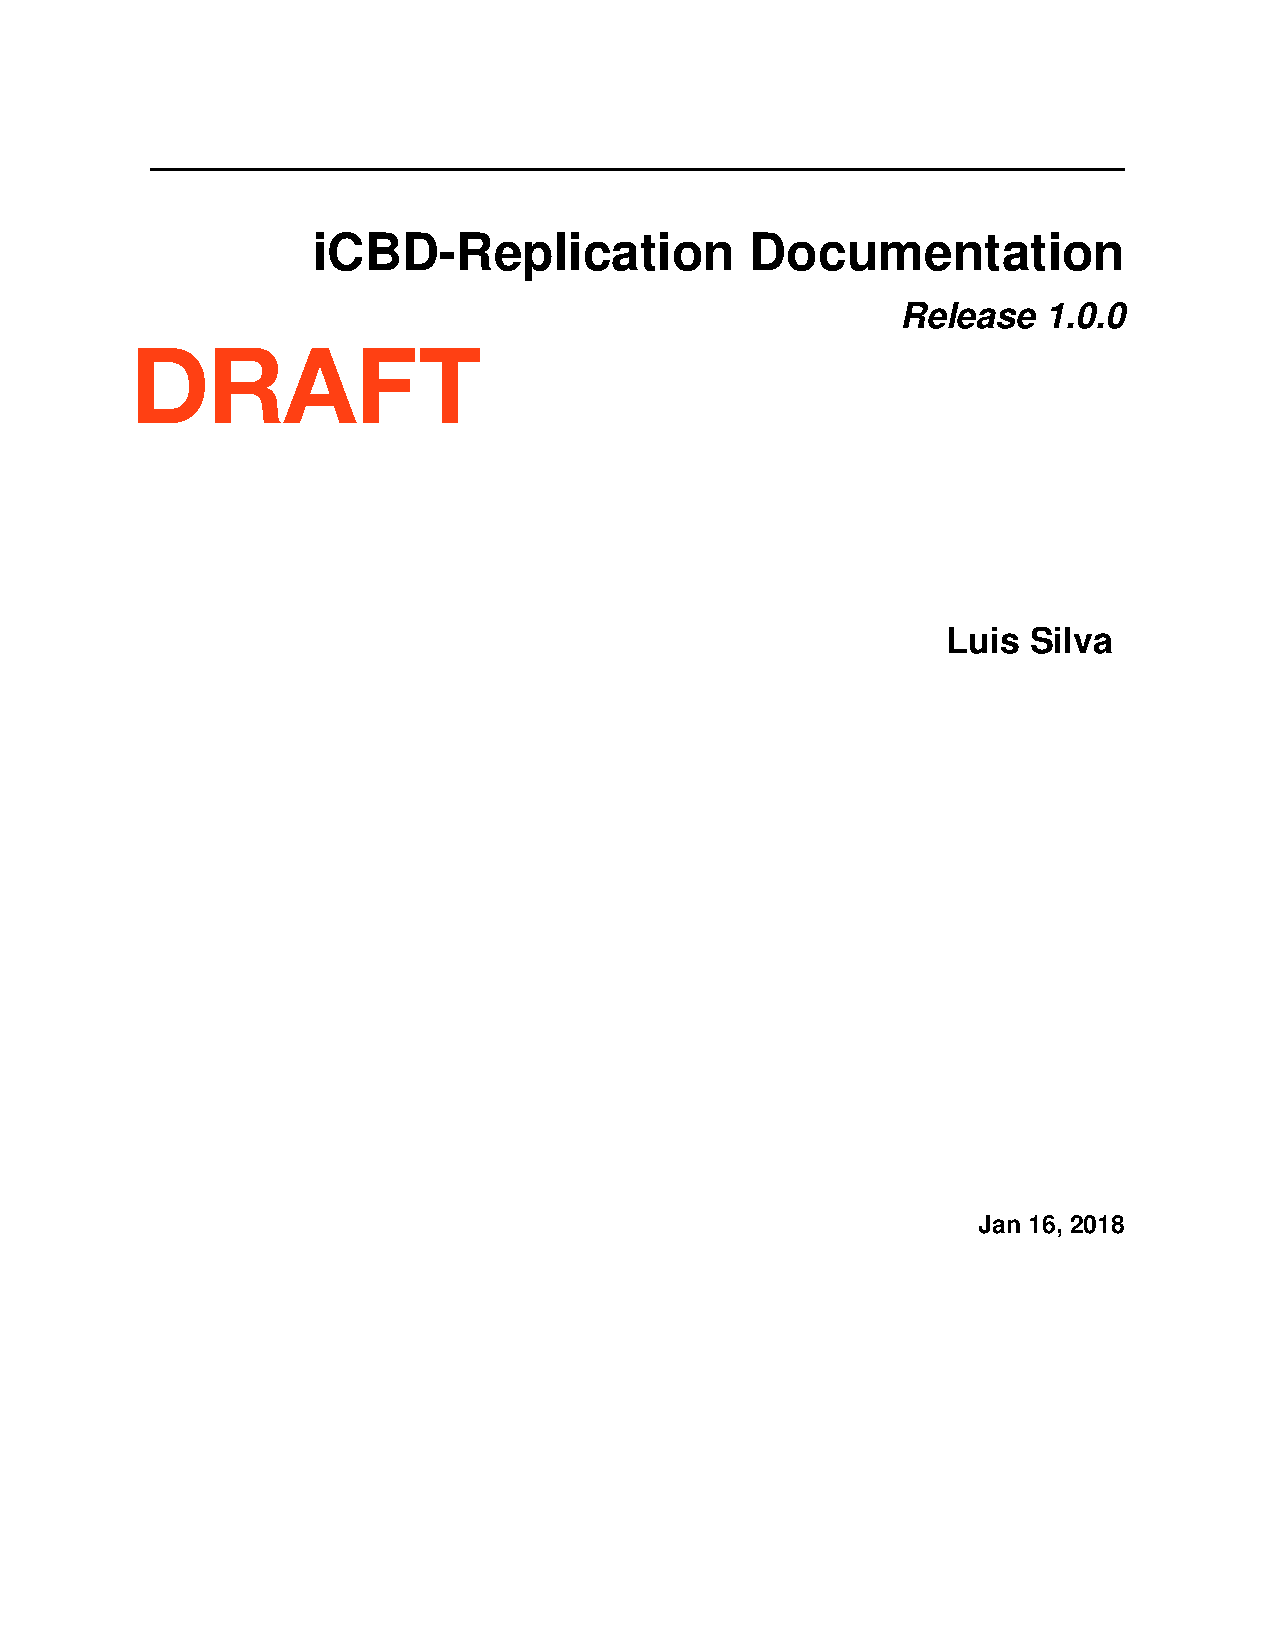
\includepdf[pages=-]{./Chapters/Annex/iCBD-Replication_exemple_draft.pdf}
%!TEX root = ../template.tex
%%%%%%%%%%%%%%%%%%%%%%%%%%%%%%%%%%%%%%%%%%%%%%%%%%%%%%%%%%%%%%%%%%%%
%% annex2.tex
%% NOVA thesis document file
%%
%% Chapter with example of appendix with a short dummy text
%%%%%%%%%%%%%%%%%%%%%%%%%%%%%%%%%%%%%%%%%%%%%%%%%%%%%%%%%%%%%%%%%%%%
\chapter{Annex 2 iCBD Installation Guide}
\label{ann:icdb_install}

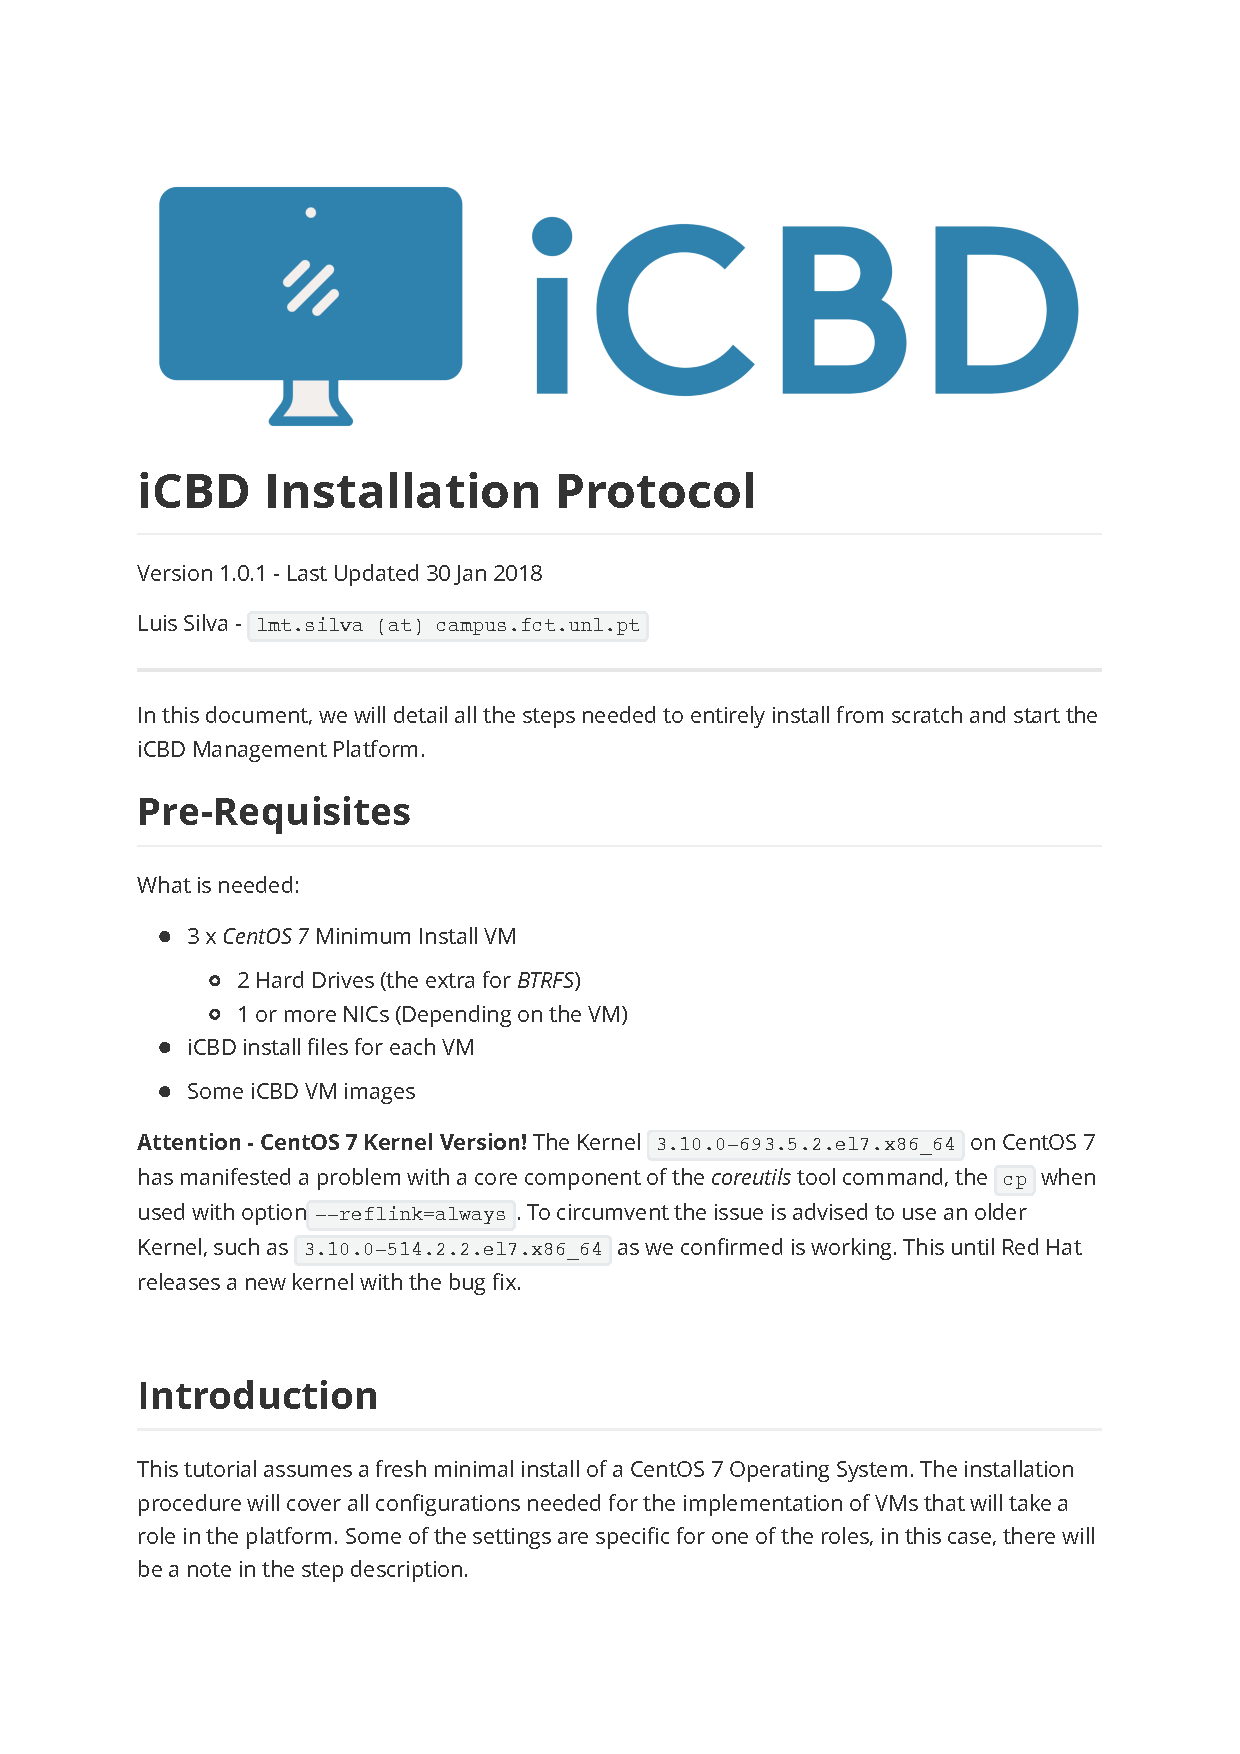
\includepdf[pages=-]{./Chapters/Annex/icbd_instalation_protocol_PDF.pdf}
%!TEX root = ../template.tex
%%%%%%%%%%%%%%%%%%%%%%%%%%%%%%%%%%%%%%%%%%%%%%%%%%%%%%%%%%%%%%%%%%%%
%% annex3.tex
%% NOVA thesis document file
%%
%% Chapter with example of appendix with a short dummy text
%%%%%%%%%%%%%%%%%%%%%%%%%%%%%%%%%%%%%%%%%%%%%%%%%%%%%%%%%%%%%%%%%%%%
\chapter{Bug on BTRFS affecting CoreUtils tool}
\label{ann:bug}

\section{Bug Report}
\label{sec:bug_report}

The bug was reported in both \textit{CentOS Bug Tracker} and \textit{Red Hat Bugzilla} on 4 of December of 2017.

\paragraph{Description of problem:}

In a CentOS 7 VM with kernel \texttt{3.10.0-693.5.2.el7.x86\_64} including a mounted disk formatted with BTRFS and btrfs-progs v4.9.1.
When executing a copy of files with the command \texttt{"cp --reflink=always"} the command fails with the indication \textit{"failed to clone 'someFile': Operation not supported"}

\paragraph{Issue:}

The above-mentioned copy fails, but in the files are created with zero bytes in the destination folder.
While trying to find the cause, it seems to be some bug in the ioctl operation. A strace log of the copy operation can be found in the uploaded files.

This problem only manifests itself in the kernel \texttt{3.10.0-693.5.2.el7.x86\_64}. If the same operation is executed in the system with the kernel \texttt{3.10.0-514.2.2.el7.x86\_64} all goes well.
More evidence that this is probably a bug introduced in this version of the kernel can be found in the git repository in the first commit of the new kernel~\footnote{https://git.centos.org/commit/rpms!kernel.git/d6bfd60741b14479a15b43acaa1ea5a8d73df543}.
In the file "SPECS/kernel.spec" line 15011~\footnote{https://git.centos.org/blob/rpms!kernel.git/d6bfd60741b14479a15b43acaa1ea5a8d73df543/SPECS!kernel.spec\#L15011} that some changes were made in the ioctl - \textit{"[fs] btrfs: fix uninit variable in clone ioctl (Bill O'Donnell) [1298680]"}

As a workaround, an older version of the kernel can be used, but this is not optimal, as future releases may have the same problem.

\paragraph{How reproducible:}

It is always reproducible. Happens every time.

\paragraph{Steps to Reproduce:}

\begin{enumerate}
	\item In a BTRFS mount execute:
	\item \texttt{dd if=/dev/urandom of=testb bs=1024k seek=1024 count=128}
	\item \texttt{cp --reflink=always testb testb\_copy}
\end{enumerate}

\paragraph{Actual results:}
The copy operation returns with "failed to clone 'testb': Operation not supported" and creates a zero bytes file in the destination of the copy.

\paragraph{Expected results:}

A clone of the file, looking precisely the same as the original with the same size.

\begin{listing}[ht]
\inputminted{bash}{./Chapters/Code/annex3_strace.sh}
\caption{Strace of the \texttt{cp --reflink=always} command}
\label{listing:bug_strace}
\end{listing}


\section{Resolution}
\label{sec:resolution}
On 5 of April of 2018, the problem was acknowledged by Red Hat, and a patch was provided. However, also informed that the fix would not be included in later RHEL7 releases, due to Red Hat deciding to deprecate BTRFS as of RHEL7.5.

\begin{listing}[ht]
\inputminted{diff}{./Chapters/Code/annex3_btrfspatch.diff}
\caption{BTRFS patch on a/fs/btrfs/super.c}
\label{listing:bug_btrfsdiff}
\end{listing}

%!TEX root = ../template.tex
%%%%%%%%%%%%%%%%%%%%%%%%%%%%%%%%%%%%%%%%%%%%%%%%%%%%%%%%%%%%%%%%%%%%
%% glossary.tex
%% NOVA thesis document file
%%
%% Acronyms definition
%%%%%%%%%%%%%%%%%%%%%%%%%%%%%%%%%%%%%%%%%%%%%%%%%%%%%%%%%%%%%%%%%%%%
\newacronym{VDI}{VDI}{Virtual Desktop Infrastructure}
\newacronym{VM}{VM}{Virtual Machine}
\newacronym{IaaS}{IaaS}{Infrastructure as a Service}

\newacronym{abbrev}{abbrev}{abbreviation of a longer text}
\newacronym{xpt}{xpto}{and extension of a xpto xpto xpto xpto xpto xpto xpto xpto xpto xpto xpto xpto xpto xpto xpto xpto xpto xpto xpto}
%!TEX root = ../template.tex
%%%%%%%%%%%%%%%%%%%%%%%%%%%%%%%%%%%%%%%%%%%%%%%%%%%%%%%%%%%%%%%%%%%%
%% glossary.tex
%% NOVA thesis document file
%%
%% Glossary definition
%%%%%%%%%%%%%%%%%%%%%%%%%%%%%%%%%%%%%%%%%%%%%%%%%%%%%%%%%%%%%%%%%%%%
\newglossaryentry{computer} {
	name={computer}, 
	description={An electronic device which is capable of receiving information (data) in a particular form and of performing a sequence of operations in accordance with a predetermined but variable set of procedural instructions (program) to produce a result in the form of information or signals.
}
}

\bibliography{bibliography}